%%%%%%%%%%%%%%%%%%%%%%%%%%%%%%%%%%%%%%%%%%%%%%%%%%%%%%%%%%%%%%%%%%
%%%%%%%%%%%%%%%%%%%%%%%%%%%%%%%%%%%%%%%%%%%%%%%%%%%%%%%%%%%%%%%%%%
%%%%%%%%%%%%%%%%%%%%%%%%%%%%%%%%%%%%%%%%%%%%%%%%%%%%%%%%%%%%%%%%%%
\documentclass[prc, reprint, amsmath, floatfix, linenumbers,10pt]{revtex4-1}
%%%%%%%%%%%%%%%%%%%%%%%%%%%%%%%%%%%%%%%%%%%%%%%%%%%%%%%%%%%%%%%%%%
%%%%%%%%%%%%%%%%%%%%%%%%%%%%%%%%%%%%%%%%%%%%%%%%%%%%%%%%%%%%%%%%%%
%%%%%%%%%%%%%%%%%%%%%%%%%%%%%%%%%%%%%%%%%%%%%%%%%%%%%%%%%%%%%%%%%%

%
% Packages
%
\usepackage[utf8]{inputenc}
\usepackage[T1]{fontenc}
\usepackage{lipsum}
\usepackage{graphicx}
\usepackage[np]{numprint}
%\usepackage{longtable}

% Gráficos em Tikz, terão que ser convertidos antes de submeter
\usepackage{tikz}
\usepackage{gnuplot-lua-tikz}

%
% Macros
%
\newcommand{\tr}{\rm{Tr}}
\newcommand{\mean}[1]{\left\langle{#1}\right\rangle}
\newcommand{\comment}[1]{{\bf\textit{#1}}}

%%%%%%%%%%%%%%%%
%%%%%%%%%%%%%%%%
\begin{document}
%%%%%%%%%%%%%%%%
%%%%%%%%%%%%%%%%

%
%%
%%%
%%%% Front Matter
%%%
%%
%

\title{The title}

\author{Clebson A. Graeff}
\affiliation{Universidade Tecnológica Federal do Paraná, campus Pato Branco \\ Via do Conhecimento, Km 1 CEP 85503-390 Pato Branco -- PR, Brazil}
\email{cgraeff@utfpr.edu.br}

\author{Débora P. Menezes}
\affiliation{Departamento de Física, Universidade Federal de Santa Catarina, Florianópolis, SC, CP 476, CEP 88.040-900, Brazil}
\email{debora.p.m@ufsc.br}

%%%

\begin{abstract}
An article usually includes an abstract, a concise summary of the work
covered at length in the main body of the article. 
\begin{description}
\item[Usage]
Secondary publications and information retrieval purposes.
\item[PACS numbers]
May be entered using the \verb+\pacs{#1}+ command.
\item[Structure]
You may use the \texttt{description} environment to structure your abstract;
use the optional argument of the \verb+\item+ command to give the category of each item. 
\end{description}
\end{abstract}

%%%

\pacs{Valid PACS appear here}

%%%

\maketitle

%
%%
%%%
%%%% Main Matter
%%%
%%
%

%%%%%%%%%%%%%%%%%%%%%%
\section{Introduction}
%%%%%%%%%%%%%%%%%%%%%%

\comment{Fazer como o Marcelo e deixar enviar a introdução em branco?}

%%%%%%%%%%%%%%%%%%%
\section{Formalism}
%%%%%%%%%%%%%%%%%%%

%%%%%%%%%%%%%%%%%%%%%%%%%
\subsection{Quark Matter}
%%%%%%%%%%%%%%%%%%%%%%%%%

The quark phase is described by a SU(2) NJL model lagrangian, including a vector term, given by\cite{Buballa2005}
\begin{equation}\label{Eq:LagNJL-SU2-Bub}
\begin{split}
	\mathcal{L} =&~ \bar{\psi}(i\gamma^\mu\partial_\mu - m_0)\psi \\
	&+ G_S[(\bar{\psi}\psi)^2 + (\bar{\psi}i\gamma_5\vec{\tau}\psi)^2] - G_V(\bar{\psi}\gamma^\mu \psi)^2.
\end{split}
\end{equation}
%
Here $\psi$ represents the quark field, $m_0$ the quark bare mass, and $G_S$ and $G_V$ are coupling constants that are chosen by fitting the pion mass $m_\pi = \np[MeV]{135.0}$ and decay constant $f_\pi = \np[MeV]{92.4}$. As the theory is non-renormalizable, a momentum cutoff $\Lambda$ is employed, which acts as a new parameter.

From the lagrangian $\mathcal{L}$, the hamiltonian density $\mathcal{H}$ can be obtained, which leads to the thermodynamic potential per volume $V$ at temperature $T$ by means of
\begin{equation}
	\omega(T, \mu) = -\frac{T}{V} \ln \tr \exp\left(-\frac{1}{T}\int d^3x(\mathcal{H} - \mu\psi^\dagger\psi\right),
\end{equation}
%
where $\tr$ stands for a trace over all states of the system, resulting in \cite{Buballa1996}
\begin{equation}\label{Eq:Pot_Termo_Temp_zero}
\begin{split}
	\omega(\mu; m, \mu_R) =&~ \omega_m^{(\rm{vac})} + \omega_m^{(\rm{med})}(\mu_R) \\
	&+ \frac{(m - m_0)^2}{4G_S} - \frac{(\mu - \mu_R)^2}{4G_V} +  \textrm{const.},
\end{split}
\end{equation}
%
with
\begin{align}
	\omega_m^{(\rm{vac})} &= -(2 n_f n_c) \int \frac{d^3p}{(2\pi)^3} E_p\\
	\omega_m^{(\rm{med})}(\mu_R) &= - (2n_f n_c) \int\frac{d^3p}{(2 \pi)^3} (\mu_R - E_p) \theta(p_F -p),
\end{align}
%
at the zero temperature limit in the mean-field approximation. Here $n_f$ and $n_c$ stand for the number of flavors and the number of colors, respectively, and $E_p = \sqrt{p^2 + m^2}$.

The renormalized chemical potential $\mu_R$ and the constituent mass $m$ are obtained by requiring that $\partial \omega / \partial \mu_R = 0$ and $\partial \omega / \partial m = 0$, respectively, resulting in
\begin{align}
	\mu_R &= \mu - 2 G_V \rho \\
	m &= m_0 - 2 G_S \rho_s
\end{align}
%
with
\begin{align}
	\rho &= n_c \rho_B = \frac{n_f n_c}{3\pi^2} p_F^3 \\
	\rho_s &= \langle \bar\psi\psi\rangle = - 2 n_f n_c \int\frac{d^3p}{(2\pi)^3} \frac{m}{E_p}(1 - \theta(p_F - p)) \\
	\mu_R &= \sqrt{p_F^2 + m^2}.
\end{align}

The constant in the potential has no physical meaning, consequently, it may be chosen so that at $T = \mu = 0$ the thermodynamic potential is zero at the value $m = m_{\rm{vac}}$ which minimizes $\omega$. This process may be represented by 
\begin{equation}
	\tilde\omega(\mu; m, \mu_R) = \omega(\mu; m, \mu_R) - \omega(0, 0; m_{\rm{vac}}, 0),
\end{equation}
%
so that the quantities we are interested in --~the pressure $p$ and the energy density $\varepsilon$~-- are obtained through
\begin{align}
		p &= -\tilde\omega(\mu; m, \mu_R) \label{Exp_pressao_T}\\
		\varepsilon &= -p + \mu \rho. \label{Exp_energia_T}
\end{align}
	
The solution of the above equations consist in determining the solution to the equation for $m$ self-consistently for each value of $\rho$ or $\mu$ (in this case $p_F = \sqrt{\mu_R^2 - m^2}\theta(\mu_R^2 - m^2)$). \comment{(+info nesse parágrafo? resultados para $\varepsilon, P$?)}

\begin{table}[!htpb]
\centering
\caption{Parameters sets for the lagrangian density~\eqref{Eq:LagNJL-SU2-Bub} \cite{Buballa1996, Buballa2005}. \label{Tab:Parametros_NJL}}
\begin{ruledtabular}
\begin{tabular}{lccccc}
Model &  $\Lambda$ & $G_S$ ($\rm{fm}^2$) & $G_V$ ($\rm{fm}^2$) & $m_0$ (MeV) & $m$ (MeV) \\
\hline
Buballa-1 & 650 & 0.19721 & -- & 0 & 313 \\
Buballa-2 & 600 & 0.26498 & -- & 0 & 400 \\
Buballa-3 & 570 & 0.34034 & -- & 0 & 500 \\
%BuballaR-1 & 664.3 & 0.18176 & $\propto G_S$ & 5.0 & 300 \\
BuballaR-2 & 587.9 & 0.27449 & $\propto G_S$ & 5.6 & 400 \\
%BuballaR-3 & 569.3 & 0.33759 & $\propto G_S$ & 5.5 & 500 \\
%BuballaR-4 & 568.6 & 0.38178 & $\propto G_S$ & 5.1 & 600
\end{tabular}
\end{ruledtabular}
\end{table}

%%%%%%%%%%%%%%%%%%%%%%%%%%
\subsection{Hadron Matter}
%%%%%%%%%%%%%%%%%%%%%%%%%%

Even though the original NJL model is unable to describe the saturation properties of the nuclear matter, this can be fixed by the inclusion of a scalar-vector channel~\cite{Koch1987}. An extended NJL model (eNJL)~\cite{Pais2016} which includes such channel is given by the lagrangian density
\begin{equation}\label{Eq:Lagrangiana_eNLJ_Pais}
\begin{split}
	\mathcal{L} =&~ \bar{\psi}(i\gamma^\mu\partial_\mu - m_0)\psi \\
	& + G_S[(\bar{\psi}\psi)^2 + (\bar{\psi}i\gamma_5\vec{\tau}\psi)^2] \\
	& - G_V(\bar{\psi}\gamma^\mu\psi)^2 - G_{sv}[(\bar{\psi}\psi)^2 + (\bar{\psi}i\gamma_5\vec{\tau}\psi)^2](\bar{\psi}\gamma^\mu\psi)^2 \\
	& - G_\rho[(\bar{\psi}\gamma^\mu\vec{\tau}\psi)^2 + (\bar{\psi}\gamma_5\gamma^\mu\vec{\tau}\psi)^2] \\
	& - G_{V\rho}(\bar{\psi}\gamma^\mu\psi)^2[(\bar{\psi}\gamma^\mu\vec{\tau}\psi)^2 + (\bar{\psi}\gamma_5\gamma^\mu\vec{\tau}\psi)^2] \\
	& - G_{S\rho} [(\bar{\psi}\psi)^2 + (\bar{\psi}i\gamma_5\vec{\tau}\psi)^2][(\bar{\psi}\gamma^\mu\vec{\tau}\psi)^2 + (\bar{\psi}\gamma_5\gamma^\mu\vec{\tau}\psi)^2].
\end{split}
\end{equation}
%

where $\psi$ represents the nucleon field and the constants $G_i$ represents the coupling constants for the different channels. The effects of the different channels are: the term in $G_V$ simulates a chiral-invariant short-range repulsion between the nucleons, the term in $G_{SV}$ accounts for the density dependence of the scalar coupling, the term in $G_\rho$ allows the description of isospin asymmetric matter, and the terms in $G_{\omega\rho}$ and $G_{S\rho}$ make the symmetry energy softer. For nuclear matter, the NJL model leads to binding, but the binding energy per particle does not have a mininum except at a rather high density where the nucleon mass is small or vanishing. The introduction of the term in $G_{SV}$ corrects this. As in the quark case, the theory is renormalized via a three momentum cutoff $\Lambda$.\comment{(Praticamente uma cópia do que está em \cite{Pais2016}).}

The thermodynamic potential is obtained from~\eqref{Eq:Lagrangiana_eNLJ_Pais} in the same way as for the quark case and is given by
\begin{equation}\label{Eq:potencial_termodinamico}
\begin{split}
	\omega(\mu) =&~ \varepsilon_{\rm{kin}} + m\rho_s - G_S\rho_s^2 + G_V\rho_B^2 + G_{sv}\rho_s^2\rho_B^2 + G_\rho\rho_3^2 \\
	&+ G_{V\rho}\rho_B^2\rho_3^2 + G_{S\rho}\rho_s^2\rho_3^2 - \mu_p\rho_B^p - \mu_n\rho_B^n,
\end{split}
\end{equation}
%
where $\rho_B$ is the total barionic density, which is the sum of the proton $\rho_B^p$ and neutron $\rho_B^n$ barionic densities, while $\rho_3 = \rho_B^p - \rho_B^n$. At zero temperature, those densities are given by
\begin{equation}
	\rho_i = \int_0^{p_F^i}\frac{dp}{\pi^2}p^2; \qquad i = p,n
\end{equation}
%
where $p_F^i$ stands for the Fermi momentum of each particle. The kinectic energy contribution is given by
\begin{equation}
	\varepsilon_{\rm{kin}} = 2 n_c \sum_i \int \frac{d^3p}{(2\pi)^3}\frac{p^2}{E_p^i}(1 - \theta(p_F^i - p))\theta(\Lambda^2 - p^2).
\end{equation}

The effective mass $m$ and the chemical potentials appearing in the thermodynamic potencial $\omega$ are determined by requiring that $\partial\omega/\partial m = 0$ and $\partial\omega/\partial p_F^i = $, resulting in
\begin{align}\label{Eq:Gap}
	m &= m_0 - 2G_s\rho_s + 2G_{sv}\rho_s\rho^2 + 2 G_{s\rho}\rho_s\rho_3^2 \\
	\mu_i &= E_{p_F}^i + 2G_v\rho + 2G_{sv}\rho\rho_s^2 \pm 2G_\rho\rho_3+2G_{v\rho}\rho_3^2\rho \nonumber \\
	&\phantom{=} \pm 2G_{v\rho}\rho^2\rho_3 \pm 2 G_{s\rho}\rho_3\rho_s^2,
\end{align}
%
with $i = p,n$, and e $E_{p_F}^i = \sqrt{M^2 + (p_F^i)^2}$. The scalar density $\rho_s$ is given by sum of the proton and neutron scalar densities
\begin{equation}
	\rho_s^i = - 2 n_c \int \frac{d^3p}{(2\pi)^3}\frac{m_0^i m_i}{E_p^i}\theta(p_F - p)\theta(\Lambda^2 - p^2)
\end{equation}
%
where $i = p, n$.

The equations of state can be obtained from
\begin{align}
	P &= -\omega(\mu) + \omega_{\rm{vac}} \\
	\varepsilon &= -P + \mu_p \rho_B^p + \mu_n \rho_B^n,
\end{align}
%
where $\omega_{\rm{vac}} = \omega(T = 0, \mu = 0, m = m_N)$, with $m_N$ representing the nucleon mass. \comment{mudei $\varepsilon_0 \to \omega_{\rm{vac}}$, ou seria melhor manter $\varepsilon_0$?} 


\begin{table*}
\caption{Conjuntos de parâmetros para a lagrangiana~\eqref{Eq:Lagrangiana_eNLJ_Pais}\cite{Pais2016}. \label{Tab:Parametros_eNJL}}
\begin{ruledtabular}
\begin{tabular}{lcccccccc}
Model & $G_s$ ($\rm{fm}^2$) & $G_v$ ($\rm{fm}^2$) & $G_{sv}$ ($\rm{fm}^8$) & $G_\rho$ ($\rm{fm}^2$) & $G_{v\rho}$ ($\rm{fm}^8$) & $G_{s\rho}$ ($\rm{fm}^8$) & $\Lambda$ (MeV) & $m$ (MeV) \\
\hline
eNJL1 & 4.855 & 4.65 & -6.583 & 0.5876 & 0 & 0 & 388.189 & 0 \\
eNJL1$\omega\rho$1 & 4.855 & 4.65 & -6.583 & 0.5976 & -1 & 0 & 388.189 & 0 \\
eNJL1$\omega\rho$2 & 4.855 & 4.65 & -6.583 & 0.6476 & -6 & 0 & 388.189 & 0 \\
eNJL2 & 3.8 & 3.8 & -4.228 & 0.6313 & 0 & 0 & 422.384 & 0 \\
eNJL2$\omega\rho$1 & 3.8 & 3.8 & -4.228 & 0.6413 & -1 & 0 & 422.384 & 0 \\
eNJL3 & 1.93 & 3.0 & -1.8 & 0.65 & 0 & 0 & 534.815 & 0 \\
eNJL3$\sigma\rho$1 & 1.93 & 3.0 & -1.8 & 0.0269 & 0 & 0.5 & 534.815 & 0 \\
eNJL1m & 1.3833 & 1.781 & -2.943 & 0.7 & 0 & 0 & 478.248 & 450 \\
eNJL1m$\sigma\rho$1 & 1.3833 & 1.781 & -2.943 & 0.0739 & 0 & 1 & 478.248 & 450 \\
eNJL2m & 1.078 & 1.955 & -2.74 & 0.75 & 0 & 0 & 502.466 & 450 \\
eNJL2m$\sigma\rho$1 & 1.078 & 1.955 & -2.74 & -0.1114 & 0 & 1 & 502.466 & 450 \\
\end{tabular}
\end{ruledtabular}
\end{table*}

%%%%%%%%%%%%%%%%%%
\section{Binodals}
%%%%%%%%%%%%%%%%%%

The QCD phase-diagram is characterized by potentially multiple phases, whose phase separation boundaries are referred as \emph{binodals}. Over those boundaries, the phases from the regions of either side of the boundary can coexist. The binodals may be determined using the Gibbs' conditions \cite{Cavagnoli2011}:
\begin{align}
\mu_B^Q &= \mu_B^H \\
T^Q &= T^H \\
P^Q &= P^H
\end{align}
%
where the indexes $H$ and $Q$ refer to the hadrons and quarks phases. The chemical potentials are given by
\begin{align}
	\mu_B^H &= \frac{\mu_p + \mu_n}{2} \\
	\mu_B^Q &= \frac{3}{2} (\mu_u + \mu_d) = 3 \mu_q.
\end{align}
%
The realized phase is the one which maximizes the pressure for a given chemical potential, consequently the phase coexistence may be obtained simply by plotting $P^i \times \mu_B^i$, $i = Q, H$, and looking for the intersection of both lines (see Fig.~\ref{Fig:Intersection}). The absence of intersections imply that there are no phase transitions in the range shown (see Fig.~\ref{Fig:NoIntersection}).

\begin{figure}
	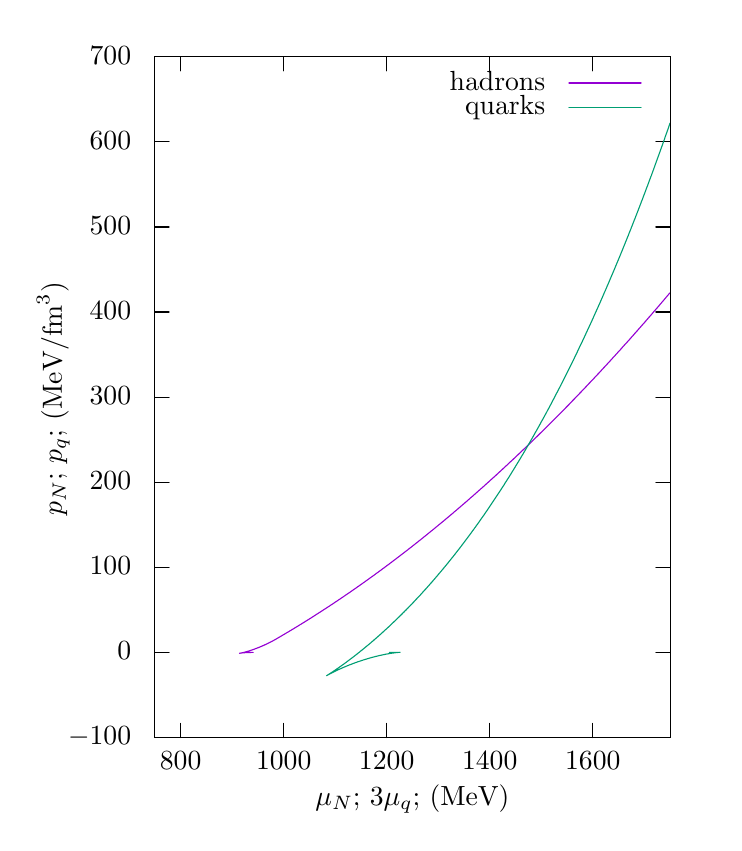
\begin{tikzpicture}[gnuplot]
%% generated with GNUPLOT 5.0p4 (Lua 5.2; terminal rev. 99, script rev. 100)
%% Thu Sep 29 16:33:14 2016
\path (0.000,0.000) rectangle (8.600,10.000);
\gpcolor{color=gp lt color border}
\gpsetlinetype{gp lt border}
\gpsetdashtype{gp dt solid}
\gpsetlinewidth{1.00}
\draw[gp path] (1.504,0.985)--(1.684,0.985);
\draw[gp path] (8.047,0.985)--(7.867,0.985);
\node[gp node right] at (1.320,0.985) {$-100$};
\draw[gp path] (1.504,2.066)--(1.684,2.066);
\draw[gp path] (8.047,2.066)--(7.867,2.066);
\node[gp node right] at (1.320,2.066) {$0$};
\draw[gp path] (1.504,3.147)--(1.684,3.147);
\draw[gp path] (8.047,3.147)--(7.867,3.147);
\node[gp node right] at (1.320,3.147) {$100$};
\draw[gp path] (1.504,4.227)--(1.684,4.227);
\draw[gp path] (8.047,4.227)--(7.867,4.227);
\node[gp node right] at (1.320,4.227) {$200$};
\draw[gp path] (1.504,5.308)--(1.684,5.308);
\draw[gp path] (8.047,5.308)--(7.867,5.308);
\node[gp node right] at (1.320,5.308) {$300$};
\draw[gp path] (1.504,6.389)--(1.684,6.389);
\draw[gp path] (8.047,6.389)--(7.867,6.389);
\node[gp node right] at (1.320,6.389) {$400$};
\draw[gp path] (1.504,7.469)--(1.684,7.469);
\draw[gp path] (8.047,7.469)--(7.867,7.469);
\node[gp node right] at (1.320,7.469) {$500$};
\draw[gp path] (1.504,8.550)--(1.684,8.550);
\draw[gp path] (8.047,8.550)--(7.867,8.550);
\node[gp node right] at (1.320,8.550) {$600$};
\draw[gp path] (1.504,9.631)--(1.684,9.631);
\draw[gp path] (8.047,9.631)--(7.867,9.631);
\node[gp node right] at (1.320,9.631) {$700$};
\draw[gp path] (1.831,0.985)--(1.831,1.165);
\draw[gp path] (1.831,9.631)--(1.831,9.451);
\node[gp node center] at (1.831,0.677) {$800$};
\draw[gp path] (3.140,0.985)--(3.140,1.165);
\draw[gp path] (3.140,9.631)--(3.140,9.451);
\node[gp node center] at (3.140,0.677) {$1000$};
\draw[gp path] (4.448,0.985)--(4.448,1.165);
\draw[gp path] (4.448,9.631)--(4.448,9.451);
\node[gp node center] at (4.448,0.677) {$1200$};
\draw[gp path] (5.757,0.985)--(5.757,1.165);
\draw[gp path] (5.757,9.631)--(5.757,9.451);
\node[gp node center] at (5.757,0.677) {$1400$};
\draw[gp path] (7.066,0.985)--(7.066,1.165);
\draw[gp path] (7.066,9.631)--(7.066,9.451);
\node[gp node center] at (7.066,0.677) {$1600$};
\draw[gp path] (1.504,9.631)--(1.504,0.985)--(8.047,0.985)--(8.047,9.631)--cycle;
\node[gp node center,rotate=-270] at (0.246,5.308) {$p_N$; $p_q$; ($\rm{MeV}/\rm{fm}^3$)};
\node[gp node center] at (4.775,0.215) {$\mu_N$; $3\mu_q$; (MeV)};
\node[gp node right] at (6.579,9.297) {hadrons};
\gpcolor{rgb color={0.580,0.000,0.827}}
\draw[gp path] (6.763,9.297)--(7.679,9.297);
\draw[gp path] (2.728,2.066)--(2.736,2.066)--(2.745,2.066)--(2.753,2.066)--(2.722,2.066)%
  --(2.730,2.066)--(2.738,2.066)--(2.745,2.066)--(2.714,2.065)--(2.722,2.066)--(2.729,2.066)%
  --(2.736,2.066)--(2.744,2.066)--(2.713,2.065)--(2.720,2.065)--(2.727,2.066)--(2.734,2.066)%
  --(2.704,2.065)--(2.711,2.065)--(2.718,2.065)--(2.725,2.066)--(2.694,2.065)--(2.701,2.065)%
  --(2.709,2.065)--(2.716,2.065)--(2.685,2.065)--(2.692,2.065)--(2.699,2.065)--(2.706,2.065)%
  --(2.713,2.065)--(2.683,2.064)--(2.690,2.065)--(2.697,2.065)--(2.704,2.065)--(2.673,2.064)%
  --(2.680,2.064)--(2.688,2.065)--(2.695,2.065)--(2.664,2.064)--(2.671,2.064)--(2.679,2.064)%
  --(2.686,2.065)--(2.693,2.065)--(2.662,2.063)--(2.670,2.064)--(2.677,2.064)--(2.684,2.065)%
  --(2.653,2.063)--(2.661,2.063)--(2.668,2.064)--(2.675,2.064)--(2.645,2.062)--(2.652,2.063)%
  --(2.659,2.063)--(2.667,2.064)--(2.674,2.064)--(2.644,2.062)--(2.651,2.063)--(2.658,2.063)%
  --(2.665,2.064)--(2.635,2.062)--(2.643,2.062)--(2.650,2.063)--(2.657,2.063)--(2.627,2.061)%
  --(2.635,2.062)--(2.642,2.062)--(2.649,2.063)--(2.657,2.063)--(2.627,2.061)--(2.634,2.061)%
  --(2.642,2.062)--(2.649,2.063)--(2.619,2.060)--(2.627,2.061)--(2.634,2.061)--(2.641,2.062)%
  --(2.612,2.060)--(2.619,2.060)--(2.627,2.061)--(2.634,2.061)--(2.642,2.062)--(2.612,2.059)%
  --(2.619,2.060)--(2.627,2.061)--(2.635,2.062)--(2.605,2.059)--(2.613,2.059)--(2.620,2.060)%
  --(2.628,2.061)--(2.598,2.058)--(2.606,2.059)--(2.613,2.060)--(2.621,2.060)--(2.629,2.061)%
  --(2.599,2.058)--(2.607,2.059)--(2.615,2.060)--(2.622,2.061)--(2.593,2.057)--(2.601,2.058)%
  --(2.609,2.059)--(2.616,2.060)--(2.624,2.061)--(2.595,2.057)--(2.603,2.058)--(2.610,2.059)%
  --(2.618,2.060)--(2.589,2.057)--(2.597,2.058)--(2.605,2.059)--(2.612,2.060)--(2.620,2.060)%
  --(2.591,2.057)--(2.599,2.058)--(2.607,2.059)--(2.615,2.060)--(2.586,2.056)--(2.594,2.057)%
  --(2.602,2.058)--(2.610,2.059)--(2.581,2.055)--(2.589,2.056)--(2.597,2.058)--(2.605,2.059)%
  --(2.613,2.060)--(2.584,2.056)--(2.592,2.057)--(2.600,2.058)--(2.608,2.059)--(2.580,2.055)%
  --(2.588,2.056)--(2.596,2.057)--(2.604,2.059)--(2.612,2.060)--(2.583,2.056)--(2.591,2.057)%
  --(2.599,2.058)--(2.607,2.059)--(2.579,2.055)--(2.587,2.056)--(2.595,2.057)--(2.603,2.059)%
  --(2.612,2.060)--(2.583,2.055)--(2.592,2.057)--(2.600,2.058)--(2.608,2.059)--(2.580,2.055)%
  --(2.588,2.056)--(2.596,2.057)--(2.604,2.059)--(2.613,2.060)--(2.585,2.056)--(2.593,2.057)%
  --(2.601,2.058)--(2.609,2.060)--(2.582,2.055)--(2.590,2.056)--(2.598,2.058)--(2.606,2.059)%
  --(2.579,2.054)--(2.587,2.056)--(2.595,2.057)--(2.604,2.059)--(2.612,2.060)--(2.585,2.055)%
  --(2.593,2.057)--(2.601,2.058)--(2.609,2.060)--(2.582,2.055)--(2.591,2.056)--(2.599,2.058)%
  --(2.607,2.060)--(2.616,2.061)--(2.588,2.056)--(2.597,2.058)--(2.605,2.059)--(2.614,2.061)%
  --(2.587,2.056)--(2.595,2.057)--(2.603,2.059)--(2.612,2.061)--(2.620,2.062)--(2.593,2.057)%
  --(2.602,2.059)--(2.610,2.060)--(2.619,2.062)--(2.592,2.056)--(2.600,2.058)--(2.609,2.060)%
  --(2.617,2.062)--(2.626,2.064)--(2.599,2.058)--(2.608,2.060)--(2.616,2.062)--(2.625,2.063)%
  --(2.598,2.058)--(2.607,2.060)--(2.616,2.061)--(2.624,2.063)--(2.598,2.057)--(2.606,2.059)%
  --(2.615,2.061)--(2.624,2.063)--(2.632,2.065)--(2.606,2.059)--(2.615,2.061)--(2.623,2.063)%
  --(2.632,2.065)--(2.606,2.059)--(2.614,2.061)--(2.623,2.063)--(2.632,2.065)--(2.640,2.067)%
  --(2.614,2.061)--(2.623,2.063)--(2.632,2.065)--(2.641,2.067)--(2.615,2.061)--(2.623,2.063)%
  --(2.632,2.065)--(2.641,2.068)--(2.615,2.061)--(2.624,2.063)--(2.633,2.066)--(2.642,2.068)%
  --(2.650,2.070)--(2.625,2.063)--(2.633,2.066)--(2.642,2.068)--(2.651,2.070)--(2.626,2.064)%
  --(2.634,2.066)--(2.643,2.068)--(2.652,2.071)--(2.661,2.073)--(2.636,2.066)--(2.645,2.069)%
  --(2.653,2.071)--(2.662,2.073)--(2.637,2.067)--(2.646,2.069)--(2.655,2.071)--(2.664,2.074)%
  --(2.639,2.067)--(2.648,2.069)--(2.657,2.072)--(2.666,2.074)--(2.675,2.077)--(2.650,2.070)%
  --(2.659,2.072)--(2.668,2.075)--(2.676,2.077)--(2.652,2.070)--(2.661,2.073)--(2.670,2.075)%
  --(2.679,2.078)--(2.654,2.071)--(2.663,2.074)--(2.672,2.076)--(2.681,2.079)--(2.690,2.081)%
  --(2.674,2.077)--(2.683,2.079)--(2.675,2.077)--(2.684,2.080)--(2.677,2.078)--(2.686,2.080)%
  --(2.678,2.078)--(2.687,2.081)--(2.680,2.078)--(2.689,2.081)--(2.681,2.079)--(2.690,2.082)%
  --(2.683,2.079)--(2.692,2.082)--(2.685,2.080)--(2.694,2.083)--(2.703,2.085)--(2.696,2.083)%
  --(2.705,2.086)--(2.697,2.084)--(2.707,2.087)--(2.699,2.084)--(2.708,2.087)--(2.701,2.085)%
  --(2.710,2.088)--(2.703,2.086)--(2.712,2.088)--(2.705,2.086)--(2.714,2.089)--(2.707,2.087)%
  --(2.716,2.090)--(2.709,2.088)--(2.719,2.091)--(2.712,2.088)--(2.721,2.091)--(2.714,2.089)%
  --(2.723,2.092)--(2.716,2.090)--(2.725,2.093)--(2.735,2.096)--(2.728,2.094)--(2.737,2.097)%
  --(2.730,2.094)--(2.739,2.097)--(2.733,2.095)--(2.742,2.098)--(2.735,2.096)--(2.744,2.099)%
  --(2.738,2.097)--(2.747,2.100)--(2.740,2.098)--(2.750,2.101)--(2.743,2.099)--(2.752,2.102)%
  --(2.746,2.100)--(2.755,2.103)--(2.749,2.101)--(2.758,2.104)--(2.752,2.102)--(2.761,2.105)%
  --(2.755,2.103)--(2.764,2.106)--(2.757,2.104)--(2.767,2.107)--(2.761,2.105)--(2.770,2.108)%
  --(2.764,2.106)--(2.773,2.109)--(2.767,2.107)--(2.776,2.111)--(2.770,2.108)--(2.779,2.112)%
  --(2.773,2.110)--(2.783,2.113)--(2.777,2.111)--(2.786,2.114)--(2.780,2.112)--(2.789,2.116)%
  --(2.783,2.113)--(2.793,2.117)--(2.787,2.115)--(2.796,2.118)--(2.790,2.116)--(2.800,2.120)%
  --(2.794,2.117)--(2.803,2.121)--(2.798,2.119)--(2.807,2.122)--(2.801,2.120)--(2.796,2.118)%
  --(2.805,2.122)--(2.800,2.119)--(2.809,2.123)--(2.804,2.121)--(2.813,2.125)--(2.807,2.123)%
  --(2.817,2.126)--(2.811,2.124)--(2.821,2.128)--(2.816,2.126)--(2.825,2.130)--(2.820,2.127)%
  --(2.829,2.131)--(2.824,2.129)--(2.833,2.133)--(2.828,2.131)--(2.823,2.129)--(2.832,2.133)%
  --(2.827,2.130)--(2.837,2.134)--(2.832,2.132)--(2.841,2.136)--(2.836,2.134)--(2.846,2.138)%
  --(2.841,2.136)--(2.850,2.140)--(2.845,2.138)--(2.855,2.142)--(2.850,2.140)--(2.845,2.138)%
  --(2.855,2.142)--(2.850,2.140)--(2.859,2.144)--(2.855,2.142)--(2.864,2.146)--(2.860,2.144)%
  --(2.855,2.142)--(2.865,2.146)--(2.860,2.144)--(2.870,2.148)--(2.865,2.146)--(2.875,2.151)%
  --(2.870,2.149)--(2.880,2.153)--(2.876,2.151)--(2.871,2.149)--(2.881,2.153)--(2.877,2.151)%
  --(2.886,2.156)--(2.882,2.154)--(2.878,2.152)--(2.888,2.156)--(2.884,2.154)--(2.893,2.159)%
  --(2.889,2.157)--(2.899,2.161)--(2.895,2.159)--(2.891,2.158)--(2.901,2.162)--(2.897,2.160)%
  --(2.906,2.165)--(2.903,2.163)--(2.899,2.161)--(2.909,2.166)--(2.905,2.164)--(2.901,2.162)%
  --(2.911,2.167)--(2.908,2.165)--(2.917,2.170)--(2.914,2.168)--(2.910,2.167)--(2.920,2.171)%
  --(2.917,2.170)--(2.926,2.174)--(2.923,2.173)--(2.920,2.171)--(2.930,2.176)--(2.927,2.174)%
  --(2.924,2.173)--(2.933,2.177)--(2.930,2.176)--(2.928,2.175)--(2.937,2.179)--(2.934,2.178)%
  --(2.932,2.177)--(2.941,2.181)--(2.939,2.180)--(2.936,2.179)--(2.946,2.183)--(2.943,2.182)%
  --(2.941,2.181)--(2.950,2.186)--(2.948,2.185)--(2.946,2.184)--(2.956,2.188)--(2.950,2.186)%
  --(2.954,2.188)--(2.958,2.190)--(2.956,2.189)--(2.960,2.190)--(2.958,2.190)--(2.962,2.191)%
  --(2.960,2.191)--(2.964,2.193)--(2.963,2.192)--(2.967,2.194)--(2.971,2.196)--(2.969,2.195)%
  --(2.973,2.197)--(2.972,2.197)--(2.976,2.199)--(2.975,2.198)--(2.974,2.198)--(2.978,2.200)%
  --(2.977,2.199)--(2.981,2.201)--(2.985,2.203)--(2.984,2.203)--(2.988,2.205)--(2.987,2.205)%
  --(2.992,2.207)--(2.996,2.209)--(2.997,2.209)--(3.002,2.212)--(3.003,2.213)--(3.004,2.213)%
  --(3.004,2.214)--(3.005,2.214)--(3.006,2.215)--(3.007,2.215)--(3.008,2.216)--(3.010,2.216)%
  --(3.011,2.217)--(3.013,2.218)--(3.014,2.219)--(3.016,2.220)--(3.018,2.221)--(3.020,2.222)%
  --(3.018,2.221)--(3.020,2.222)--(3.023,2.224)--(3.022,2.223)--(3.024,2.224)--(3.025,2.225)%
  --(3.026,2.225)--(3.027,2.226)--(3.029,2.227)--(3.030,2.228)--(3.031,2.228)--(3.032,2.229)%
  --(3.034,2.230)--(3.036,2.231)--(3.038,2.232)--(3.040,2.233)--(3.041,2.234)--(3.042,2.234)%
  --(3.042,2.235)--(3.043,2.235)--(3.044,2.236)--(3.047,2.237)--(3.056,2.243)--(3.066,2.248)%
  --(3.075,2.254)--(3.084,2.259)--(3.094,2.265)--(3.103,2.270)--(3.113,2.276)--(3.122,2.281)%
  --(3.131,2.287)--(3.141,2.292)--(3.150,2.298)--(3.160,2.303)--(3.169,2.309)--(3.178,2.315)%
  --(3.188,2.320)--(3.197,2.326)--(3.207,2.331)--(3.216,2.337)--(3.225,2.343)--(3.235,2.348)%
  --(3.244,2.354)--(3.254,2.360)--(3.263,2.365)--(3.272,2.371)--(3.282,2.377)--(3.291,2.382)%
  --(3.300,2.388)--(3.310,2.394)--(3.319,2.399)--(3.329,2.405)--(3.338,2.411)--(3.347,2.417)%
  --(3.357,2.422)--(3.366,2.428)--(3.375,2.434)--(3.385,2.440)--(3.394,2.446)--(3.403,2.451)%
  --(3.413,2.457)--(3.422,2.463)--(3.432,2.469)--(3.441,2.475)--(3.450,2.481)--(3.460,2.486)%
  --(3.469,2.492)--(3.478,2.498)--(3.488,2.504)--(3.497,2.510)--(3.506,2.516)--(3.516,2.522)%
  --(3.525,2.528)--(3.534,2.534)--(3.544,2.540)--(3.553,2.546)--(3.562,2.552)--(3.572,2.558)%
  --(3.581,2.564)--(3.590,2.570)--(3.600,2.576)--(3.609,2.582)--(3.618,2.588)--(3.628,2.594)%
  --(3.637,2.600)--(3.646,2.606)--(3.655,2.612)--(3.665,2.618)--(3.674,2.624)--(3.683,2.630)%
  --(3.693,2.636)--(3.702,2.642)--(3.711,2.648)--(3.721,2.654)--(3.730,2.661)--(3.739,2.667)%
  --(3.749,2.673)--(3.758,2.679)--(3.767,2.685)--(3.776,2.691)--(3.786,2.698)--(3.795,2.704)%
  --(3.804,2.710)--(3.814,2.716)--(3.823,2.722)--(3.832,2.729)--(3.841,2.735)--(3.851,2.741)%
  --(3.860,2.747)--(3.869,2.754)--(3.879,2.760)--(3.888,2.766)--(3.897,2.773)--(3.906,2.779)%
  --(3.916,2.785)--(3.925,2.792)--(3.934,2.798)--(3.943,2.804)--(3.953,2.811)--(3.962,2.817)%
  --(3.971,2.823)--(3.981,2.830)--(3.990,2.836)--(3.999,2.843)--(4.008,2.849)--(4.018,2.855)%
  --(4.027,2.862)--(4.036,2.868)--(4.045,2.875)--(4.055,2.881)--(4.064,2.888)--(4.073,2.894)%
  --(4.082,2.901)--(4.092,2.907)--(4.101,2.914)--(4.110,2.920)--(4.119,2.927)--(4.129,2.933)%
  --(4.138,2.940)--(4.147,2.946)--(4.156,2.953)--(4.166,2.959)--(4.175,2.966)--(4.184,2.973)%
  --(4.193,2.979)--(4.203,2.986)--(4.212,2.992)--(4.221,2.999)--(4.230,3.006)--(4.239,3.012)%
  --(4.249,3.019)--(4.258,3.026)--(4.267,3.032)--(4.276,3.039)--(4.286,3.046)--(4.295,3.052)%
  --(4.304,3.059)--(4.313,3.066)--(4.322,3.073)--(4.332,3.079)--(4.341,3.086)--(4.350,3.093)%
  --(4.359,3.100)--(4.369,3.106)--(4.378,3.113)--(4.387,3.120)--(4.396,3.127)--(4.405,3.134)%
  --(4.415,3.140)--(4.424,3.147)--(4.433,3.154)--(4.442,3.161)--(4.451,3.168)--(4.461,3.175)%
  --(4.470,3.181)--(4.479,3.188)--(4.488,3.195)--(4.497,3.202)--(4.507,3.209)--(4.516,3.216)%
  --(4.525,3.223)--(4.534,3.230)--(4.543,3.237)--(4.553,3.244)--(4.562,3.251)--(4.571,3.258)%
  --(4.580,3.265)--(4.589,3.272)--(4.598,3.279)--(4.608,3.286)--(4.617,3.293)--(4.626,3.300)%
  --(4.635,3.307)--(4.644,3.314)--(4.653,3.321)--(4.663,3.328)--(4.672,3.335)--(4.681,3.342)%
  --(4.690,3.349)--(4.699,3.356)--(4.709,3.363)--(4.718,3.371)--(4.727,3.378)--(4.736,3.385)%
  --(4.745,3.392)--(4.754,3.399)--(4.764,3.406)--(4.773,3.414)--(4.782,3.421)--(4.791,3.428)%
  --(4.800,3.435)--(4.809,3.442)--(4.818,3.450)--(4.828,3.457)--(4.837,3.464)--(4.846,3.471)%
  --(4.855,3.479)--(4.864,3.486)--(4.873,3.493)--(4.883,3.500)--(4.892,3.508)--(4.901,3.515)%
  --(4.910,3.522)--(4.919,3.530)--(4.928,3.537)--(4.937,3.544)--(4.947,3.552)--(4.956,3.559)%
  --(4.965,3.567)--(4.974,3.574)--(4.983,3.581)--(4.992,3.589)--(5.001,3.596)--(5.010,3.604)%
  --(5.020,3.611)--(5.029,3.618)--(5.038,3.626)--(5.047,3.633)--(5.056,3.641)--(5.065,3.648)%
  --(5.074,3.656)--(5.084,3.663)--(5.093,3.671)--(5.102,3.678)--(5.111,3.686)--(5.120,3.693)%
  --(5.129,3.701)--(5.138,3.708)--(5.147,3.716)--(5.157,3.724)--(5.166,3.731)--(5.175,3.739)%
  --(5.184,3.746)--(5.193,3.754)--(5.202,3.762)--(5.211,3.769)--(5.220,3.777)--(5.229,3.784)%
  --(5.239,3.792)--(5.248,3.800)--(5.257,3.807)--(5.266,3.815)--(5.275,3.823)--(5.284,3.830)%
  --(5.293,3.838)--(5.302,3.846)--(5.311,3.854)--(5.320,3.861)--(5.330,3.869)--(5.339,3.877)%
  --(5.348,3.885)--(5.357,3.892)--(5.366,3.900)--(5.375,3.908)--(5.384,3.916)--(5.393,3.924)%
  --(5.402,3.931)--(5.411,3.939)--(5.420,3.947)--(5.430,3.955)--(5.439,3.963)--(5.448,3.971)%
  --(5.457,3.978)--(5.466,3.986)--(5.475,3.994)--(5.484,4.002)--(5.493,4.010)--(5.502,4.018)%
  --(5.511,4.026)--(5.520,4.034)--(5.530,4.042)--(5.539,4.050)--(5.548,4.058)--(5.557,4.066)%
  --(5.566,4.074)--(5.575,4.082)--(5.584,4.090)--(5.593,4.098)--(5.602,4.106)--(5.611,4.114)%
  --(5.620,4.122)--(5.629,4.130)--(5.638,4.138)--(5.647,4.146)--(5.657,4.154)--(5.666,4.162)%
  --(5.675,4.170)--(5.684,4.178)--(5.693,4.186)--(5.702,4.195)--(5.711,4.203)--(5.720,4.211)%
  --(5.729,4.219)--(5.738,4.227)--(5.747,4.235)--(5.756,4.243)--(5.765,4.252)--(5.774,4.260)%
  --(5.783,4.268)--(5.792,4.276)--(5.801,4.284)--(5.811,4.293)--(5.820,4.301)--(5.829,4.309)%
  --(5.838,4.317)--(5.847,4.326)--(5.856,4.334)--(5.865,4.342)--(5.874,4.351)--(5.883,4.359)%
  --(5.892,4.367)--(5.901,4.376)--(5.910,4.384)--(5.919,4.392)--(5.928,4.401)--(5.937,4.409)%
  --(5.946,4.417)--(5.955,4.426)--(5.964,4.434)--(5.973,4.442)--(5.982,4.451)--(5.991,4.459)%
  --(6.000,4.468)--(6.009,4.476)--(6.018,4.485)--(6.028,4.493)--(6.037,4.502)--(6.046,4.510)%
  --(6.055,4.518)--(6.064,4.527)--(6.073,4.535)--(6.082,4.544)--(6.091,4.552)--(6.100,4.561)%
  --(6.109,4.570)--(6.118,4.578)--(6.127,4.587)--(6.136,4.595)--(6.145,4.604)--(6.154,4.612)%
  --(6.163,4.621)--(6.172,4.630)--(6.181,4.638)--(6.190,4.647)--(6.199,4.655)--(6.208,4.664)%
  --(6.217,4.673)--(6.226,4.681)--(6.235,4.690)--(6.244,4.699)--(6.253,4.707)--(6.262,4.716)%
  --(6.271,4.725)--(6.280,4.733)--(6.289,4.742)--(6.298,4.751)--(6.307,4.760)--(6.316,4.768)%
  --(6.325,4.777)--(6.334,4.786)--(6.343,4.795)--(6.352,4.803)--(6.361,4.812)--(6.370,4.821)%
  --(6.379,4.830)--(6.388,4.839)--(6.397,4.848)--(6.406,4.856)--(6.415,4.865)--(6.424,4.874)%
  --(6.433,4.883)--(6.442,4.892)--(6.451,4.901)--(6.460,4.910)--(6.469,4.918)--(6.478,4.927)%
  --(6.487,4.936)--(6.496,4.945)--(6.505,4.954)--(6.514,4.963)--(6.523,4.972)--(6.532,4.981)%
  --(6.541,4.990)--(6.550,4.999)--(6.559,5.008)--(6.568,5.017)--(6.577,5.026)--(6.586,5.035)%
  --(6.595,5.044)--(6.604,5.053)--(6.613,5.062)--(6.622,5.071)--(6.631,5.080)--(6.640,5.089)%
  --(6.649,5.098)--(6.658,5.108)--(6.667,5.117)--(6.676,5.126)--(6.685,5.135)--(6.694,5.144)%
  --(6.703,5.153)--(6.712,5.162)--(6.721,5.171)--(6.730,5.181)--(6.739,5.190)--(6.748,5.199)%
  --(6.757,5.208)--(6.766,5.217)--(6.775,5.227)--(6.784,5.236)--(6.792,5.245)--(6.801,5.254)%
  --(6.810,5.264)--(6.819,5.273)--(6.828,5.282)--(6.837,5.291)--(6.846,5.301)--(6.855,5.310)%
  --(6.864,5.319)--(6.873,5.329)--(6.882,5.338)--(6.891,5.347)--(6.900,5.357)--(6.909,5.366)%
  --(6.918,5.375)--(6.927,5.385)--(6.936,5.394)--(6.945,5.403)--(6.954,5.413)--(6.963,5.422)%
  --(6.972,5.432)--(6.981,5.441)--(6.990,5.451)--(6.999,5.460)--(7.008,5.469)--(7.016,5.479)%
  --(7.025,5.488)--(7.034,5.498)--(7.043,5.507)--(7.052,5.517)--(7.061,5.526)--(7.070,5.536)%
  --(7.079,5.545)--(7.088,5.555)--(7.097,5.564)--(7.106,5.574)--(7.115,5.584)--(7.124,5.593)%
  --(7.133,5.603)--(7.142,5.612)--(7.151,5.622)--(7.160,5.632)--(7.169,5.641)--(7.177,5.651)%
  --(7.186,5.660)--(7.195,5.670)--(7.204,5.680)--(7.213,5.689)--(7.222,5.699)--(7.231,5.709)%
  --(7.240,5.718)--(7.249,5.728)--(7.258,5.738)--(7.267,5.748)--(7.276,5.757)--(7.285,5.767)%
  --(7.294,5.777)--(7.303,5.787)--(7.312,5.796)--(7.320,5.806)--(7.329,5.816)--(7.338,5.826)%
  --(7.347,5.835)--(7.356,5.845)--(7.365,5.855)--(7.374,5.865)--(7.383,5.875)--(7.392,5.885)%
  --(7.401,5.894)--(7.410,5.904)--(7.419,5.914)--(7.428,5.924)--(7.436,5.934)--(7.445,5.944)%
  --(7.454,5.954)--(7.463,5.964)--(7.472,5.974)--(7.481,5.984)--(7.490,5.993)--(7.499,6.003)%
  --(7.508,6.013)--(7.517,6.023)--(7.526,6.033)--(7.535,6.043)--(7.544,6.053)--(7.552,6.063)%
  --(7.561,6.073)--(7.570,6.083)--(7.579,6.093)--(7.588,6.103)--(7.597,6.114)--(7.606,6.124)%
  --(7.615,6.134)--(7.624,6.144)--(7.633,6.154)--(7.642,6.164)--(7.650,6.174)--(7.659,6.184)%
  --(7.668,6.194)--(7.677,6.204)--(7.686,6.215)--(7.695,6.225)--(7.704,6.235)--(7.713,6.245)%
  --(7.722,6.255)--(7.731,6.265)--(7.740,6.276)--(7.748,6.286)--(7.757,6.296)--(7.766,6.306)%
  --(7.775,6.317)--(7.784,6.327)--(7.793,6.337)--(7.802,6.347)--(7.811,6.358)--(7.820,6.368)%
  --(7.828,6.378)--(7.837,6.389)--(7.846,6.399)--(7.855,6.409)--(7.864,6.420)--(7.873,6.430)%
  --(7.882,6.440)--(7.891,6.451)--(7.900,6.461)--(7.909,6.471)--(7.917,6.482)--(7.926,6.492)%
  --(7.935,6.502)--(7.944,6.513)--(7.953,6.523)--(7.962,6.534)--(7.971,6.544)--(7.980,6.555)%
  --(7.989,6.565)--(7.997,6.576)--(8.006,6.586)--(8.015,6.597)--(8.024,6.607)--(8.033,6.618)%
  --(8.042,6.628)--(8.047,6.634);
\gpcolor{color=gp lt color border}
\node[gp node right] at (6.579,8.989) {quarks};
\gpcolor{rgb color={0.000,0.620,0.451}}
\draw[gp path] (6.763,8.989)--(7.679,8.989);
\draw[gp path] (4.482,2.066)--(4.515,2.066)--(4.537,2.066)--(4.554,2.066)--(4.566,2.066)%
  --(4.577,2.066)--(4.585,2.067)--(4.593,2.067)--(4.598,2.067)--(4.603,2.067)--(4.607,2.067)%
  --(4.611,2.067)--(4.614,2.067)--(4.616,2.067)--(4.617,2.068)--(4.618,2.068)--(4.619,2.068)%
  --(4.618,2.068)--(4.617,2.067)--(4.616,2.067)--(4.614,2.067)--(4.612,2.067)--(4.610,2.067)%
  --(4.608,2.067)--(4.606,2.067)--(4.603,2.066)--(4.601,2.066)--(4.598,2.066)--(4.595,2.066)%
  --(4.592,2.065)--(4.588,2.065)--(4.585,2.065)--(4.581,2.064)--(4.577,2.064)--(4.573,2.063)%
  --(4.569,2.063)--(4.565,2.063)--(4.561,2.062)--(4.557,2.062)--(4.552,2.061)--(4.548,2.060)%
  --(4.543,2.060)--(4.539,2.059)--(4.534,2.059)--(4.529,2.058)--(4.524,2.057)--(4.519,2.057)%
  --(4.514,2.056)--(4.509,2.055)--(4.504,2.054)--(4.499,2.053)--(4.493,2.053)--(4.488,2.052)%
  --(4.483,2.051)--(4.477,2.050)--(4.472,2.049)--(4.466,2.048)--(4.460,2.047)--(4.455,2.046)%
  --(4.449,2.045)--(4.443,2.044)--(4.437,2.043)--(4.431,2.042)--(4.425,2.040)--(4.419,2.039)%
  --(4.413,2.038)--(4.408,2.037)--(4.402,2.036)--(4.395,2.034)--(4.389,2.033)--(4.383,2.032)%
  --(4.377,2.030)--(4.371,2.029)--(4.364,2.028)--(4.358,2.026)--(4.352,2.025)--(4.345,2.023)%
  --(4.339,2.022)--(4.332,2.020)--(4.326,2.019)--(4.319,2.017)--(4.313,2.015)--(4.306,2.014)%
  --(4.300,2.012)--(4.293,2.010)--(4.287,2.009)--(4.280,2.007)--(4.273,2.005)--(4.267,2.003)%
  --(4.260,2.002)--(4.253,2.000)--(4.247,1.998)--(4.240,1.996)--(4.233,1.994)--(4.227,1.992)%
  --(4.220,1.990)--(4.213,1.988)--(4.206,1.986)--(4.200,1.984)--(4.193,1.982)--(4.186,1.980)%
  --(4.179,1.978)--(4.172,1.976)--(4.166,1.974)--(4.159,1.972)--(4.152,1.970)--(4.145,1.967)%
  --(4.138,1.965)--(4.131,1.963)--(4.125,1.961)--(4.118,1.958)--(4.111,1.956)--(4.104,1.954)%
  --(4.097,1.951)--(4.090,1.949)--(4.083,1.947)--(4.077,1.944)--(4.070,1.942)--(4.063,1.940)%
  --(4.056,1.937)--(4.049,1.935)--(4.043,1.932)--(4.036,1.930)--(4.029,1.927)--(4.022,1.925)%
  --(4.016,1.922)--(4.009,1.920)--(4.002,1.917)--(3.995,1.914)--(3.989,1.912)--(3.982,1.909)%
  --(3.975,1.907)--(3.969,1.904)--(3.962,1.901)--(3.956,1.899)--(3.949,1.896)--(3.943,1.893)%
  --(3.936,1.891)--(3.930,1.888)--(3.923,1.885)--(3.917,1.882)--(3.910,1.880)--(3.904,1.877)%
  --(3.898,1.874)--(3.891,1.872)--(3.885,1.869)--(3.879,1.866)--(3.873,1.863)--(3.867,1.861)%
  --(3.861,1.858)--(3.855,1.855)--(3.849,1.853)--(3.843,1.850)--(3.837,1.847)--(3.831,1.845)%
  --(3.825,1.842)--(3.820,1.839)--(3.814,1.837)--(3.808,1.834)--(3.803,1.831)--(3.798,1.829)%
  --(3.792,1.826)--(3.787,1.824)--(3.782,1.821)--(3.777,1.819)--(3.772,1.816)--(3.767,1.814)%
  --(3.762,1.811)--(3.757,1.809)--(3.753,1.807)--(3.748,1.804)--(3.744,1.802)--(3.740,1.800)%
  --(3.736,1.798)--(3.732,1.796)--(3.728,1.794)--(3.724,1.792)--(3.720,1.790)--(3.717,1.788)%
  --(3.714,1.786)--(3.710,1.785)--(3.707,1.783)--(3.705,1.781)--(3.702,1.780)--(3.699,1.779)%
  --(3.697,1.777)--(3.695,1.776)--(3.693,1.775)--(3.691,1.774)--(3.690,1.773)--(3.688,1.772)%
  --(3.687,1.772)--(3.686,1.771)--(3.685,1.771)--(3.685,1.770)--(3.684,1.770)--(3.685,1.770)%
  --(3.685,1.771)--(3.686,1.771)--(3.687,1.772)--(3.689,1.773)--(3.690,1.773)--(3.692,1.775)%
  --(3.694,1.776)--(3.696,1.777)--(3.698,1.779)--(3.701,1.780)--(3.704,1.782)--(3.707,1.784)%
  --(3.710,1.786)--(3.714,1.788)--(3.718,1.791)--(3.722,1.793)--(3.726,1.796)--(3.730,1.799)%
  --(3.735,1.802)--(3.739,1.805)--(3.744,1.808)--(3.749,1.811)--(3.755,1.815)--(3.760,1.818)%
  --(3.766,1.822)--(3.771,1.826)--(3.777,1.830)--(3.783,1.834)--(3.789,1.838)--(3.796,1.842)%
  --(3.802,1.847)--(3.809,1.851)--(3.815,1.856)--(3.822,1.860)--(3.829,1.865)--(3.836,1.870)%
  --(3.843,1.875)--(3.850,1.880)--(3.857,1.885)--(3.864,1.890)--(3.872,1.895)--(3.879,1.901)%
  --(3.887,1.906)--(3.894,1.911)--(3.902,1.917)--(3.909,1.922)--(3.917,1.928)--(3.925,1.934)%
  --(3.933,1.939)--(3.940,1.945)--(3.948,1.951)--(3.956,1.957)--(3.964,1.963)--(3.972,1.969)%
  --(3.980,1.975)--(3.988,1.981)--(3.996,1.987)--(4.004,1.993)--(4.013,2.000)--(4.021,2.006)%
  --(4.029,2.012)--(4.037,2.018)--(4.045,2.025)--(4.053,2.031)--(4.062,2.038)--(4.070,2.044)%
  --(4.078,2.051)--(4.086,2.057)--(4.095,2.064)--(4.103,2.070)--(4.111,2.077)--(4.119,2.084)%
  --(4.128,2.090)--(4.136,2.097)--(4.144,2.104)--(4.153,2.110)--(4.161,2.117)--(4.169,2.124)%
  --(4.177,2.131)--(4.186,2.138)--(4.194,2.145)--(4.202,2.151)--(4.211,2.158)--(4.219,2.165)%
  --(4.227,2.172)--(4.235,2.179)--(4.244,2.186)--(4.252,2.193)--(4.260,2.200)--(4.268,2.207)%
  --(4.277,2.214)--(4.285,2.221)--(4.293,2.229)--(4.301,2.236)--(4.309,2.243)--(4.318,2.250)%
  --(4.326,2.257)--(4.334,2.264)--(4.342,2.272)--(4.350,2.279)--(4.358,2.286)--(4.367,2.293)%
  --(4.375,2.301)--(4.383,2.308)--(4.391,2.315)--(4.399,2.323)--(4.407,2.330)--(4.415,2.337)%
  --(4.423,2.345)--(4.431,2.352)--(4.439,2.359)--(4.448,2.367)--(4.456,2.374)--(4.464,2.382)%
  --(4.472,2.389)--(4.480,2.396)--(4.488,2.404)--(4.496,2.411)--(4.503,2.419)--(4.511,2.426)%
  --(4.519,2.434)--(4.527,2.442)--(4.535,2.449)--(4.543,2.457)--(4.551,2.464)--(4.559,2.472)%
  --(4.567,2.479)--(4.575,2.487)--(4.582,2.495)--(4.590,2.502)--(4.598,2.510)--(4.606,2.517)%
  --(4.614,2.525)--(4.621,2.533)--(4.629,2.540)--(4.637,2.548)--(4.645,2.556)--(4.652,2.564)%
  --(4.660,2.571)--(4.668,2.579)--(4.676,2.587)--(4.683,2.595)--(4.691,2.602)--(4.699,2.610)%
  --(4.706,2.618)--(4.714,2.626)--(4.722,2.633)--(4.729,2.641)--(4.737,2.649)--(4.744,2.657)%
  --(4.752,2.665)--(4.759,2.673)--(4.767,2.680)--(4.775,2.688)--(4.782,2.696)--(4.790,2.704)%
  --(4.797,2.712)--(4.805,2.720)--(4.812,2.728)--(4.819,2.736)--(4.827,2.744)--(4.834,2.752)%
  --(4.842,2.760)--(4.849,2.768)--(4.857,2.776)--(4.864,2.783)--(4.871,2.791)--(4.879,2.799)%
  --(4.886,2.807)--(4.893,2.816)--(4.901,2.824)--(4.908,2.832)--(4.915,2.840)--(4.923,2.848)%
  --(4.930,2.856)--(4.937,2.864)--(4.945,2.872)--(4.952,2.880)--(4.959,2.888)--(4.966,2.896)%
  --(4.973,2.904)--(4.981,2.912)--(4.988,2.920)--(4.995,2.929)--(5.002,2.937)--(5.009,2.945)%
  --(5.017,2.953)--(5.024,2.961)--(5.031,2.969)--(5.038,2.978)--(5.045,2.986)--(5.052,2.994)%
  --(5.059,3.002)--(5.066,3.010)--(5.073,3.019)--(5.080,3.027)--(5.087,3.035)--(5.094,3.043)%
  --(5.101,3.052)--(5.108,3.060)--(5.115,3.068)--(5.122,3.076)--(5.129,3.085)--(5.136,3.093)%
  --(5.143,3.101)--(5.150,3.110)--(5.157,3.118)--(5.164,3.126)--(5.171,3.135)--(5.178,3.143)%
  --(5.185,3.151)--(5.192,3.160)--(5.198,3.168)--(5.205,3.176)--(5.212,3.185)--(5.219,3.193)%
  --(5.226,3.201)--(5.233,3.210)--(5.239,3.218)--(5.246,3.227)--(5.253,3.235)--(5.260,3.244)%
  --(5.267,3.252)--(5.273,3.260)--(5.280,3.269)--(5.287,3.277)--(5.294,3.286)--(5.300,3.294)%
  --(5.307,3.303)--(5.314,3.311)--(5.320,3.320)--(5.327,3.328)--(5.334,3.337)--(5.340,3.345)%
  --(5.347,3.354)--(5.354,3.362)--(5.360,3.371)--(5.367,3.379)--(5.373,3.388)--(5.380,3.396)%
  --(5.387,3.405)--(5.393,3.414)--(5.400,3.422)--(5.406,3.431)--(5.413,3.439)--(5.419,3.448)%
  --(5.426,3.457)--(5.432,3.465)--(5.439,3.474)--(5.445,3.482)--(5.452,3.491)--(5.458,3.500)%
  --(5.465,3.508)--(5.471,3.517)--(5.478,3.526)--(5.484,3.534)--(5.491,3.543)--(5.497,3.552)%
  --(5.504,3.560)--(5.510,3.569)--(5.516,3.578)--(5.523,3.586)--(5.529,3.595)--(5.535,3.604)%
  --(5.542,3.613)--(5.548,3.621)--(5.555,3.630)--(5.561,3.639)--(5.567,3.648)--(5.574,3.656)%
  --(5.580,3.665)--(5.586,3.674)--(5.592,3.683)--(5.599,3.691)--(5.605,3.700)--(5.611,3.709)%
  --(5.618,3.718)--(5.624,3.727)--(5.630,3.735)--(5.636,3.744)--(5.642,3.753)--(5.649,3.762)%
  --(5.655,3.771)--(5.661,3.780)--(5.667,3.788)--(5.673,3.797)--(5.680,3.806)--(5.686,3.815)%
  --(5.692,3.824)--(5.698,3.833)--(5.704,3.842)--(5.710,3.851)--(5.717,3.859)--(5.723,3.868)%
  --(5.729,3.877)--(5.735,3.886)--(5.741,3.895)--(5.747,3.904)--(5.753,3.913)--(5.759,3.922)%
  --(5.765,3.931)--(5.771,3.940)--(5.777,3.949)--(5.783,3.958)--(5.789,3.967)--(5.795,3.976)%
  --(5.801,3.985)--(5.807,3.994)--(5.813,4.003)--(5.819,4.012)--(5.825,4.021)--(5.831,4.030)%
  --(5.837,4.039)--(5.843,4.048)--(5.849,4.057)--(5.855,4.066)--(5.861,4.075)--(5.867,4.084)%
  --(5.873,4.093)--(5.879,4.102)--(5.885,4.111)--(5.891,4.120)--(5.897,4.129)--(5.903,4.139)%
  --(5.908,4.148)--(5.914,4.157)--(5.920,4.166)--(5.926,4.175)--(5.932,4.184)--(5.938,4.193)%
  --(5.944,4.202)--(5.949,4.212)--(5.955,4.221)--(5.961,4.230)--(5.967,4.239)--(5.973,4.248)%
  --(5.978,4.257)--(5.984,4.266)--(5.990,4.276)--(5.996,4.285)--(6.002,4.294)--(6.007,4.303)%
  --(6.013,4.312)--(6.019,4.322)--(6.025,4.331)--(6.030,4.340)--(6.036,4.349)--(6.042,4.359)%
  --(6.047,4.368)--(6.053,4.377)--(6.059,4.386)--(6.065,4.396)--(6.070,4.405)--(6.076,4.414)%
  --(6.082,4.423)--(6.087,4.433)--(6.093,4.442)--(6.099,4.451)--(6.104,4.461)--(6.110,4.470)%
  --(6.115,4.479)--(6.121,4.488)--(6.127,4.498)--(6.132,4.507)--(6.138,4.516)--(6.144,4.526)%
  --(6.149,4.535)--(6.155,4.544)--(6.160,4.554)--(6.166,4.563)--(6.171,4.573)--(6.177,4.582)%
  --(6.183,4.591)--(6.188,4.601)--(6.194,4.610)--(6.199,4.619)--(6.205,4.629)--(6.210,4.638)%
  --(6.216,4.648)--(6.221,4.657)--(6.227,4.666)--(6.232,4.676)--(6.238,4.685)--(6.243,4.695)%
  --(6.249,4.704)--(6.254,4.714)--(6.260,4.723)--(6.265,4.733)--(6.270,4.742)--(6.276,4.751)%
  --(6.281,4.761)--(6.287,4.770)--(6.292,4.780)--(6.298,4.789)--(6.303,4.799)--(6.308,4.808)%
  --(6.314,4.818)--(6.319,4.827)--(6.325,4.837)--(6.330,4.846)--(6.335,4.856)--(6.341,4.866)%
  --(6.346,4.875)--(6.352,4.885)--(6.357,4.894)--(6.362,4.904)--(6.368,4.913)--(6.373,4.923)%
  --(6.378,4.932)--(6.384,4.942)--(6.389,4.952)--(6.394,4.961)--(6.400,4.971)--(6.405,4.980)%
  --(6.410,4.990)--(6.415,5.000)--(6.421,5.009)--(6.426,5.019)--(6.431,5.028)--(6.437,5.038)%
  --(6.442,5.048)--(6.447,5.057)--(6.452,5.067)--(6.458,5.077)--(6.463,5.086)--(6.468,5.096)%
  --(6.473,5.106)--(6.479,5.115)--(6.484,5.125)--(6.489,5.135)--(6.494,5.144)--(6.499,5.154)%
  --(6.505,5.164)--(6.510,5.173)--(6.515,5.183)--(6.520,5.193)--(6.525,5.203)--(6.531,5.212)%
  --(6.536,5.222)--(6.541,5.232)--(6.546,5.241)--(6.551,5.251)--(6.556,5.261)--(6.561,5.271)%
  --(6.567,5.280)--(6.572,5.290)--(6.577,5.300)--(6.582,5.310)--(6.587,5.320)--(6.592,5.329)%
  --(6.597,5.339)--(6.602,5.349)--(6.607,5.359)--(6.613,5.369)--(6.618,5.378)--(6.623,5.388)%
  --(6.628,5.398)--(6.633,5.408)--(6.638,5.418)--(6.643,5.427)--(6.648,5.437)--(6.653,5.447)%
  --(6.658,5.457)--(6.663,5.467)--(6.668,5.477)--(6.673,5.487)--(6.678,5.496)--(6.683,5.506)%
  --(6.688,5.516)--(6.693,5.526)--(6.698,5.536)--(6.703,5.546)--(6.708,5.556)--(6.713,5.566)%
  --(6.718,5.576)--(6.723,5.586)--(6.728,5.595)--(6.733,5.605)--(6.738,5.615)--(6.743,5.625)%
  --(6.748,5.635)--(6.753,5.645)--(6.758,5.655)--(6.763,5.665)--(6.768,5.675)--(6.773,5.685)%
  --(6.778,5.695)--(6.783,5.705)--(6.788,5.715)--(6.792,5.725)--(6.797,5.735)--(6.802,5.745)%
  --(6.807,5.755)--(6.812,5.765)--(6.817,5.775)--(6.822,5.785)--(6.827,5.795)--(6.832,5.805)%
  --(6.836,5.815)--(6.841,5.825)--(6.846,5.835)--(6.851,5.845)--(6.856,5.855)--(6.861,5.865)%
  --(6.866,5.875)--(6.870,5.885)--(6.875,5.895)--(6.880,5.905)--(6.885,5.915)--(6.890,5.925)%
  --(6.894,5.936)--(6.899,5.946)--(6.904,5.956)--(6.909,5.966)--(6.914,5.976)--(6.918,5.986)%
  --(6.923,5.996)--(6.928,6.006)--(6.933,6.016)--(6.938,6.027)--(6.942,6.037)--(6.947,6.047)%
  --(6.952,6.057)--(6.957,6.067)--(6.961,6.077)--(6.966,6.087)--(6.971,6.098)--(6.976,6.108)%
  --(6.980,6.118)--(6.985,6.128)--(6.990,6.138)--(6.995,6.148)--(6.999,6.159)--(7.004,6.169)%
  --(7.009,6.179)--(7.013,6.189)--(7.018,6.199)--(7.023,6.210)--(7.027,6.220)--(7.032,6.230)%
  --(7.037,6.240)--(7.042,6.251)--(7.046,6.261)--(7.051,6.271)--(7.056,6.281)--(7.060,6.291)%
  --(7.065,6.302)--(7.070,6.312)--(7.074,6.322)--(7.079,6.333)--(7.083,6.343)--(7.088,6.353)%
  --(7.093,6.363)--(7.097,6.374)--(7.102,6.384)--(7.107,6.394)--(7.111,6.405)--(7.116,6.415)%
  --(7.120,6.425)--(7.125,6.435)--(7.130,6.446)--(7.134,6.456)--(7.139,6.466)--(7.143,6.477)%
  --(7.148,6.487)--(7.153,6.497)--(7.157,6.508)--(7.162,6.518)--(7.166,6.528)--(7.171,6.539)%
  --(7.175,6.549)--(7.180,6.560)--(7.185,6.570)--(7.189,6.580)--(7.194,6.591)--(7.198,6.601)%
  --(7.203,6.611)--(7.207,6.622)--(7.212,6.632)--(7.216,6.643)--(7.221,6.653)--(7.225,6.663)%
  --(7.230,6.674)--(7.234,6.684)--(7.239,6.695)--(7.243,6.705)--(7.248,6.716)--(7.252,6.726)%
  --(7.257,6.736)--(7.261,6.747)--(7.266,6.757)--(7.270,6.768)--(7.275,6.778)--(7.279,6.789)%
  --(7.284,6.799)--(7.288,6.810)--(7.293,6.820)--(7.297,6.831)--(7.302,6.841)--(7.306,6.852)%
  --(7.311,6.862)--(7.315,6.873)--(7.319,6.883)--(7.324,6.894)--(7.328,6.904)--(7.333,6.915)%
  --(7.337,6.925)--(7.342,6.936)--(7.346,6.946)--(7.350,6.957)--(7.355,6.967)--(7.359,6.978)%
  --(7.364,6.988)--(7.368,6.999)--(7.372,7.009)--(7.377,7.020)--(7.381,7.031)--(7.386,7.041)%
  --(7.390,7.052)--(7.394,7.062)--(7.399,7.073)--(7.403,7.083)--(7.408,7.094)--(7.412,7.105)%
  --(7.416,7.115)--(7.421,7.126)--(7.425,7.136)--(7.429,7.147)--(7.434,7.158)--(7.438,7.168)%
  --(7.442,7.179)--(7.447,7.190)--(7.451,7.200)--(7.455,7.211)--(7.460,7.222)--(7.464,7.232)%
  --(7.468,7.243)--(7.473,7.253)--(7.477,7.264)--(7.481,7.275)--(7.486,7.285)--(7.490,7.296)%
  --(7.494,7.307)--(7.498,7.317)--(7.503,7.328)--(7.507,7.339)--(7.511,7.350)--(7.516,7.360)%
  --(7.520,7.371)--(7.524,7.382)--(7.528,7.392)--(7.533,7.403)--(7.537,7.414)--(7.541,7.425)%
  --(7.546,7.435)--(7.550,7.446)--(7.554,7.457)--(7.558,7.467)--(7.563,7.478)--(7.567,7.489)%
  --(7.571,7.500)--(7.575,7.510)--(7.579,7.521)--(7.584,7.532)--(7.588,7.543)--(7.592,7.554)%
  --(7.596,7.564)--(7.601,7.575)--(7.605,7.586)--(7.609,7.597)--(7.613,7.607)--(7.617,7.618)%
  --(7.622,7.629)--(7.626,7.640)--(7.630,7.651)--(7.634,7.661)--(7.638,7.672)--(7.643,7.683)%
  --(7.647,7.694)--(7.651,7.705)--(7.655,7.716)--(7.659,7.726)--(7.663,7.737)--(7.668,7.748)%
  --(7.672,7.759)--(7.676,7.770)--(7.680,7.781)--(7.684,7.792)--(7.688,7.802)--(7.693,7.813)%
  --(7.697,7.824)--(7.701,7.835)--(7.705,7.846)--(7.709,7.857)--(7.713,7.868)--(7.717,7.879)%
  --(7.722,7.890)--(7.726,7.900)--(7.730,7.911)--(7.734,7.922)--(7.738,7.933)--(7.742,7.944)%
  --(7.746,7.955)--(7.750,7.966)--(7.754,7.977)--(7.759,7.988)--(7.763,7.999)--(7.767,8.010)%
  --(7.771,8.021)--(7.775,8.032)--(7.779,8.043)--(7.783,8.054)--(7.787,8.064)--(7.791,8.075)%
  --(7.795,8.086)--(7.799,8.097)--(7.803,8.108)--(7.808,8.119)--(7.812,8.130)--(7.816,8.141)%
  --(7.820,8.152)--(7.824,8.163)--(7.828,8.174)--(7.832,8.185)--(7.836,8.196)--(7.840,8.207)%
  --(7.844,8.218)--(7.848,8.229)--(7.852,8.240)--(7.856,8.251)--(7.860,8.263)--(7.864,8.274)%
  --(7.868,8.285)--(7.872,8.296)--(7.876,8.307)--(7.880,8.318)--(7.884,8.329)--(7.888,8.340)%
  --(7.892,8.351)--(7.896,8.362)--(7.900,8.373)--(7.904,8.384)--(7.908,8.395)--(7.912,8.406)%
  --(7.916,8.417)--(7.920,8.429)--(7.924,8.440)--(7.928,8.451)--(7.932,8.462)--(7.936,8.473)%
  --(7.940,8.484)--(7.944,8.495)--(7.948,8.506)--(7.952,8.517)--(7.956,8.529)--(7.960,8.540)%
  --(7.964,8.551)--(7.968,8.562)--(7.972,8.573)--(7.976,8.584)--(7.980,8.595)--(7.983,8.607)%
  --(7.987,8.618)--(7.991,8.629)--(7.995,8.640)--(7.999,8.651)--(8.003,8.662)--(8.007,8.674)%
  --(8.011,8.685)--(8.015,8.696)--(8.019,8.707)--(8.023,8.718)--(8.027,8.730)--(8.031,8.741)%
  --(8.034,8.752)--(8.038,8.763)--(8.042,8.774)--(8.046,8.786)--(8.047,8.788);
\gpcolor{color=gp lt color border}
\draw[gp path] (1.504,9.631)--(1.504,0.985)--(8.047,0.985)--(8.047,9.631)--cycle;
%% coordinates of the plot area
\gpdefrectangularnode{gp plot 1}{\pgfpoint{1.504cm}{0.985cm}}{\pgfpoint{8.047cm}{9.631cm}}
\end{tikzpicture}
%% gnuplot variables

	\caption{Example of a combination of parameters sets for which there is a phase transition. Quarks: BuballaR-2; Hadrons: eNJL1$\omega\rho$1. \label{Fig:Intersection}}
\end{figure}

\begin{figure}
	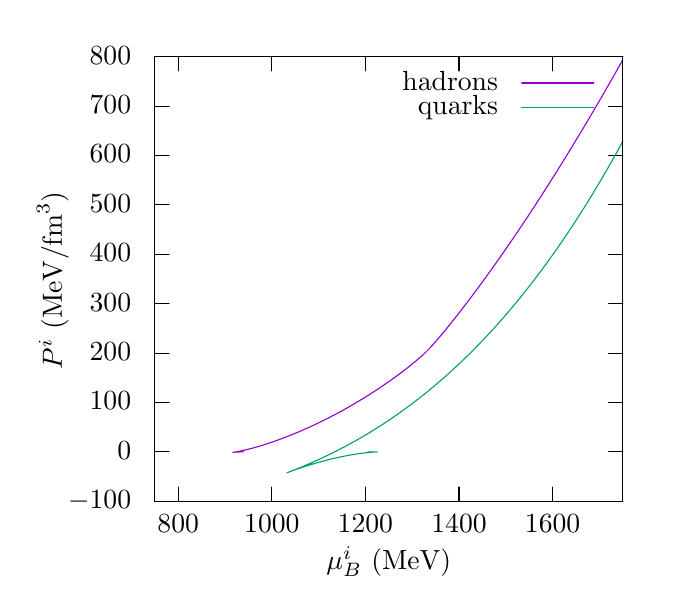
\begin{tikzpicture}[gnuplot]
%% generated with GNUPLOT 5.0p4 (Lua 5.2; terminal rev. 99, script rev. 100)
%% Wed Oct 26 17:32:28 2016
\path (0.000,0.000) rectangle (8.000,7.000);
\gpcolor{color=gp lt color border}
\gpsetlinetype{gp lt border}
\gpsetdashtype{gp dt solid}
\gpsetlinewidth{1.00}
\draw[gp path] (1.504,0.985)--(1.684,0.985);
\draw[gp path] (7.447,0.985)--(7.267,0.985);
\node[gp node right] at (1.320,0.985) {$-100$};
\draw[gp path] (1.504,1.612)--(1.684,1.612);
\draw[gp path] (7.447,1.612)--(7.267,1.612);
\node[gp node right] at (1.320,1.612) {$0$};
\draw[gp path] (1.504,2.240)--(1.684,2.240);
\draw[gp path] (7.447,2.240)--(7.267,2.240);
\node[gp node right] at (1.320,2.240) {$100$};
\draw[gp path] (1.504,2.867)--(1.684,2.867);
\draw[gp path] (7.447,2.867)--(7.267,2.867);
\node[gp node right] at (1.320,2.867) {$200$};
\draw[gp path] (1.504,3.494)--(1.684,3.494);
\draw[gp path] (7.447,3.494)--(7.267,3.494);
\node[gp node right] at (1.320,3.494) {$300$};
\draw[gp path] (1.504,4.122)--(1.684,4.122);
\draw[gp path] (7.447,4.122)--(7.267,4.122);
\node[gp node right] at (1.320,4.122) {$400$};
\draw[gp path] (1.504,4.749)--(1.684,4.749);
\draw[gp path] (7.447,4.749)--(7.267,4.749);
\node[gp node right] at (1.320,4.749) {$500$};
\draw[gp path] (1.504,5.376)--(1.684,5.376);
\draw[gp path] (7.447,5.376)--(7.267,5.376);
\node[gp node right] at (1.320,5.376) {$600$};
\draw[gp path] (1.504,6.004)--(1.684,6.004);
\draw[gp path] (7.447,6.004)--(7.267,6.004);
\node[gp node right] at (1.320,6.004) {$700$};
\draw[gp path] (1.504,6.631)--(1.684,6.631);
\draw[gp path] (7.447,6.631)--(7.267,6.631);
\node[gp node right] at (1.320,6.631) {$800$};
\draw[gp path] (1.801,0.985)--(1.801,1.165);
\draw[gp path] (1.801,6.631)--(1.801,6.451);
\node[gp node center] at (1.801,0.677) {$800$};
\draw[gp path] (2.990,0.985)--(2.990,1.165);
\draw[gp path] (2.990,6.631)--(2.990,6.451);
\node[gp node center] at (2.990,0.677) {$1000$};
\draw[gp path] (4.178,0.985)--(4.178,1.165);
\draw[gp path] (4.178,6.631)--(4.178,6.451);
\node[gp node center] at (4.178,0.677) {$1200$};
\draw[gp path] (5.367,0.985)--(5.367,1.165);
\draw[gp path] (5.367,6.631)--(5.367,6.451);
\node[gp node center] at (5.367,0.677) {$1400$};
\draw[gp path] (6.556,0.985)--(6.556,1.165);
\draw[gp path] (6.556,6.631)--(6.556,6.451);
\node[gp node center] at (6.556,0.677) {$1600$};
\draw[gp path] (1.504,6.631)--(1.504,0.985)--(7.447,0.985)--(7.447,6.631)--cycle;
\node[gp node center,rotate=-270] at (0.246,3.808) {$P^i$ ($\rm{MeV}/\rm{fm}^3$)};
\node[gp node center] at (4.475,0.215) {$\mu_B^i$ (MeV)};
\node[gp node right] at (5.979,6.297) {hadrons};
\gpcolor{rgb color={0.580,0.000,0.827}}
\draw[gp path] (6.163,6.297)--(7.079,6.297);
\draw[gp path] (2.630,1.612)--(2.629,1.612)--(2.628,1.612)--(2.627,1.612)--(2.626,1.612)%
  --(2.625,1.612)--(2.624,1.612)--(2.623,1.612)--(2.622,1.612)--(2.620,1.612)--(2.619,1.612)%
  --(2.618,1.612)--(2.616,1.612)--(2.615,1.612)--(2.613,1.612)--(2.612,1.612)--(2.610,1.612)%
  --(2.609,1.612)--(2.608,1.612)--(2.606,1.612)--(2.605,1.612)--(2.603,1.612)--(2.602,1.612)%
  --(2.600,1.612)--(2.599,1.612)--(2.597,1.612)--(2.596,1.612)--(2.594,1.612)--(2.593,1.612)%
  --(2.591,1.612)--(2.590,1.612)--(2.589,1.612)--(2.587,1.612)--(2.586,1.612)--(2.584,1.612)%
  --(2.583,1.612)--(2.582,1.612)--(2.580,1.612)--(2.579,1.612)--(2.577,1.611)--(2.576,1.611)%
  --(2.575,1.611)--(2.573,1.611)--(2.572,1.611)--(2.571,1.611)--(2.569,1.611)--(2.568,1.611)%
  --(2.567,1.611)--(2.565,1.611)--(2.564,1.611)--(2.563,1.611)--(2.561,1.611)--(2.560,1.611)%
  --(2.559,1.611)--(2.558,1.611)--(2.556,1.611)--(2.555,1.611)--(2.554,1.611)--(2.553,1.611)%
  --(2.552,1.611)--(2.550,1.611)--(2.549,1.610)--(2.548,1.610)--(2.547,1.610)--(2.546,1.610)%
  --(2.545,1.610)--(2.544,1.610)--(2.543,1.610)--(2.542,1.610)--(2.540,1.610)--(2.539,1.610)%
  --(2.538,1.610)--(2.537,1.610)--(2.536,1.610)--(2.535,1.610)--(2.534,1.610)--(2.533,1.610)%
  --(2.532,1.610)--(2.531,1.610)--(2.530,1.609)--(2.529,1.609)--(2.528,1.609)--(2.527,1.609)%
  --(2.526,1.609)--(2.525,1.609)--(2.524,1.609)--(2.523,1.609)--(2.522,1.609)--(2.521,1.609)%
  --(2.520,1.609)--(2.519,1.609)--(2.518,1.609)--(2.517,1.609)--(2.516,1.609)--(2.515,1.609)%
  --(2.515,1.608)--(2.514,1.608)--(2.513,1.608)--(2.512,1.608)--(2.511,1.608)--(2.510,1.608)%
  --(2.509,1.608)--(2.508,1.608)--(2.507,1.608)--(2.506,1.608)--(2.505,1.608)--(2.504,1.608)%
  --(2.503,1.608)--(2.502,1.608)--(2.502,1.607)--(2.501,1.607)--(2.500,1.607)--(2.499,1.607)%
  --(2.498,1.607)--(2.497,1.607)--(2.496,1.607)--(2.495,1.607)--(2.494,1.607)--(2.495,1.607)%
  --(2.496,1.607)--(2.497,1.607)--(2.498,1.607)--(2.499,1.607)--(2.500,1.607)--(2.500,1.608)%
  --(2.501,1.608)--(2.502,1.608)--(2.503,1.608)--(2.504,1.608)--(2.505,1.608)--(2.506,1.608)%
  --(2.507,1.608)--(2.507,1.609)--(2.508,1.609)--(2.509,1.609)--(2.510,1.609)--(2.511,1.609)%
  --(2.512,1.609)--(2.513,1.609)--(2.514,1.610)--(2.515,1.610)--(2.516,1.610)--(2.517,1.610)%
  --(2.518,1.610)--(2.519,1.610)--(2.520,1.611)--(2.521,1.611)--(2.522,1.611)--(2.523,1.611)%
  --(2.524,1.611)--(2.525,1.611)--(2.526,1.611)--(2.526,1.612)--(2.527,1.612)--(2.528,1.612)%
  --(2.529,1.612)--(2.530,1.612)--(2.531,1.612)--(2.532,1.612)--(2.533,1.613)--(2.534,1.613)%
  --(2.535,1.613)--(2.536,1.613)--(2.537,1.613)--(2.538,1.614)--(2.539,1.614)--(2.540,1.614)%
  --(2.541,1.614)--(2.542,1.614)--(2.543,1.614)--(2.544,1.615)--(2.545,1.615)--(2.546,1.615)%
  --(2.547,1.615)--(2.548,1.615)--(2.549,1.616)--(2.550,1.616)--(2.551,1.616)--(2.553,1.616)%
  --(2.554,1.616)--(2.555,1.617)--(2.556,1.617)--(2.557,1.617)--(2.558,1.617)--(2.559,1.617)%
  --(2.560,1.618)--(2.562,1.618)--(2.563,1.618)--(2.564,1.618)--(2.565,1.619)--(2.566,1.619)%
  --(2.568,1.619)--(2.569,1.619)--(2.570,1.619)--(2.571,1.620)--(2.573,1.620)--(2.574,1.620)%
  --(2.575,1.620)--(2.576,1.621)--(2.578,1.621)--(2.579,1.621)--(2.580,1.621)--(2.582,1.622)%
  --(2.583,1.622)--(2.584,1.622)--(2.586,1.623)--(2.587,1.623)--(2.588,1.623)--(2.590,1.623)%
  --(2.591,1.624)--(2.592,1.624)--(2.594,1.624)--(2.595,1.625)--(2.597,1.625)--(2.598,1.625)%
  --(2.599,1.625)--(2.601,1.626)--(2.602,1.626)--(2.604,1.626)--(2.605,1.627)--(2.607,1.627)%
  --(2.608,1.627)--(2.610,1.628)--(2.611,1.628)--(2.613,1.628)--(2.614,1.629)--(2.616,1.629)%
  --(2.617,1.629)--(2.619,1.630)--(2.620,1.630)--(2.622,1.630)--(2.623,1.631)--(2.625,1.631)%
  --(2.627,1.631)--(2.628,1.632)--(2.630,1.632)--(2.631,1.632)--(2.633,1.633)--(2.635,1.633)%
  --(2.636,1.634)--(2.638,1.634)--(2.640,1.634)--(2.641,1.635)--(2.643,1.635)--(2.645,1.635)%
  --(2.646,1.636)--(2.648,1.636)--(2.650,1.637)--(2.651,1.637)--(2.653,1.637)--(2.655,1.638)%
  --(2.656,1.638)--(2.658,1.639)--(2.660,1.639)--(2.662,1.639)--(2.663,1.640)--(2.665,1.640)%
  --(2.667,1.641)--(2.669,1.641)--(2.671,1.642)--(2.672,1.642)--(2.674,1.642)--(2.676,1.643)%
  --(2.678,1.643)--(2.680,1.644)--(2.681,1.644)--(2.683,1.645)--(2.685,1.645)--(2.687,1.646)%
  --(2.689,1.646)--(2.691,1.646)--(2.693,1.647)--(2.694,1.647)--(2.696,1.648)--(2.698,1.648)%
  --(2.700,1.649)--(2.702,1.649)--(2.704,1.650)--(2.706,1.650)--(2.708,1.651)--(2.710,1.651)%
  --(2.712,1.652)--(2.714,1.652)--(2.716,1.653)--(2.718,1.653)--(2.720,1.654)--(2.722,1.654)%
  --(2.724,1.655)--(2.726,1.655)--(2.728,1.656)--(2.730,1.656)--(2.732,1.657)--(2.734,1.658)%
  --(2.736,1.658)--(2.738,1.659)--(2.740,1.659)--(2.742,1.660)--(2.744,1.660)--(2.746,1.661)%
  --(2.748,1.661)--(2.750,1.662)--(2.752,1.662)--(2.754,1.663)--(2.756,1.664)--(2.758,1.664)%
  --(2.761,1.665)--(2.763,1.665)--(2.765,1.666)--(2.767,1.667)--(2.769,1.667)--(2.771,1.668)%
  --(2.773,1.668)--(2.776,1.669)--(2.778,1.670)--(2.780,1.670)--(2.782,1.671)--(2.784,1.671)%
  --(2.786,1.672)--(2.789,1.673)--(2.791,1.673)--(2.793,1.674)--(2.795,1.674)--(2.797,1.675)%
  --(2.800,1.676)--(2.802,1.676)--(2.804,1.677)--(2.806,1.678)--(2.809,1.678)--(2.811,1.679)%
  --(2.813,1.680)--(2.815,1.680)--(2.818,1.681)--(2.820,1.682)--(2.822,1.682)--(2.825,1.683)%
  --(2.827,1.684)--(2.829,1.684)--(2.831,1.685)--(2.834,1.686)--(2.836,1.686)--(2.838,1.687)%
  --(2.841,1.688)--(2.843,1.689)--(2.845,1.689)--(2.848,1.690)--(2.850,1.691)--(2.853,1.691)%
  --(2.855,1.692)--(2.857,1.693)--(2.860,1.694)--(2.862,1.694)--(2.864,1.695)--(2.867,1.696)%
  --(2.869,1.696)--(2.872,1.697)--(2.874,1.698)--(2.876,1.699)--(2.879,1.699)--(2.881,1.700)%
  --(2.884,1.701)--(2.886,1.702)--(2.889,1.702)--(2.891,1.703)--(2.894,1.704)--(2.896,1.705)%
  --(2.899,1.706)--(2.901,1.706)--(2.903,1.707)--(2.906,1.708)--(2.908,1.709)--(2.911,1.710)%
  --(2.913,1.710)--(2.916,1.711)--(2.918,1.712)--(2.921,1.713)--(2.923,1.714)--(2.926,1.714)%
  --(2.929,1.715)--(2.931,1.716)--(2.934,1.717)--(2.936,1.718)--(2.939,1.719)--(2.941,1.719)%
  --(2.944,1.720)--(2.946,1.721)--(2.949,1.722)--(2.951,1.723)--(2.954,1.724)--(2.957,1.724)%
  --(2.959,1.725)--(2.962,1.726)--(2.964,1.727)--(2.967,1.728)--(2.970,1.729)--(2.972,1.730)%
  --(2.975,1.731)--(2.977,1.731)--(2.980,1.732)--(2.983,1.733)--(2.985,1.734)--(2.988,1.735)%
  --(2.991,1.736)--(2.993,1.737)--(2.996,1.738)--(2.999,1.739)--(3.001,1.740)--(3.004,1.740)%
  --(3.007,1.741)--(3.009,1.742)--(3.012,1.743)--(3.015,1.744)--(3.017,1.745)--(3.020,1.746)%
  --(3.023,1.747)--(3.025,1.748)--(3.028,1.749)--(3.031,1.750)--(3.034,1.751)--(3.036,1.752)%
  --(3.039,1.753)--(3.042,1.754)--(3.044,1.755)--(3.047,1.756)--(3.050,1.757)--(3.053,1.758)%
  --(3.055,1.759)--(3.058,1.760)--(3.061,1.761)--(3.064,1.762)--(3.066,1.763)--(3.069,1.764)%
  --(3.072,1.765)--(3.075,1.766)--(3.077,1.767)--(3.080,1.768)--(3.083,1.769)--(3.086,1.770)%
  --(3.089,1.771)--(3.091,1.772)--(3.094,1.773)--(3.097,1.774)--(3.100,1.775)--(3.103,1.776)%
  --(3.105,1.777)--(3.108,1.778)--(3.111,1.779)--(3.114,1.780)--(3.117,1.781)--(3.120,1.782)%
  --(3.122,1.783)--(3.125,1.784)--(3.128,1.785)--(3.131,1.786)--(3.134,1.787)--(3.137,1.789)%
  --(3.139,1.790)--(3.142,1.791)--(3.145,1.792)--(3.148,1.793)--(3.151,1.794)--(3.154,1.795)%
  --(3.157,1.796)--(3.160,1.797)--(3.162,1.798)--(3.165,1.799)--(3.168,1.801)--(3.171,1.802)%
  --(3.174,1.803)--(3.177,1.804)--(3.180,1.805)--(3.183,1.806)--(3.186,1.807)--(3.188,1.808)%
  --(3.191,1.810)--(3.194,1.811)--(3.197,1.812)--(3.200,1.813)--(3.203,1.814)--(3.206,1.815)%
  --(3.209,1.817)--(3.212,1.818)--(3.215,1.819)--(3.218,1.820)--(3.221,1.821)--(3.224,1.822)%
  --(3.226,1.824)--(3.229,1.825)--(3.232,1.826)--(3.235,1.827)--(3.238,1.828)--(3.241,1.830)%
  --(3.244,1.831)--(3.247,1.832)--(3.250,1.833)--(3.253,1.834)--(3.256,1.836)--(3.259,1.837)%
  --(3.262,1.838)--(3.265,1.839)--(3.268,1.840)--(3.271,1.842)--(3.274,1.843)--(3.277,1.844)%
  --(3.280,1.845)--(3.283,1.847)--(3.286,1.848)--(3.289,1.849)--(3.292,1.850)--(3.295,1.852)%
  --(3.298,1.853)--(3.301,1.854)--(3.304,1.855)--(3.307,1.857)--(3.310,1.858)--(3.313,1.859)%
  --(3.316,1.860)--(3.319,1.862)--(3.322,1.863)--(3.325,1.864)--(3.328,1.865)--(3.331,1.867)%
  --(3.334,1.868)--(3.337,1.869)--(3.340,1.871)--(3.343,1.872)--(3.346,1.873)--(3.349,1.875)%
  --(3.352,1.876)--(3.355,1.877)--(3.358,1.878)--(3.361,1.880)--(3.365,1.881)--(3.368,1.882)%
  --(3.371,1.884)--(3.374,1.885)--(3.377,1.886)--(3.380,1.888)--(3.383,1.889)--(3.386,1.890)%
  --(3.389,1.892)--(3.392,1.893)--(3.395,1.894)--(3.398,1.896)--(3.401,1.897)--(3.404,1.899)%
  --(3.407,1.900)--(3.410,1.901)--(3.413,1.903)--(3.417,1.904)--(3.420,1.905)--(3.423,1.907)%
  --(3.426,1.908)--(3.429,1.909)--(3.432,1.911)--(3.435,1.912)--(3.438,1.914)--(3.441,1.915)%
  --(3.444,1.916)--(3.447,1.918)--(3.450,1.919)--(3.454,1.921)--(3.457,1.922)--(3.460,1.923)%
  --(3.463,1.925)--(3.466,1.926)--(3.469,1.928)--(3.472,1.929)--(3.475,1.930)--(3.478,1.932)%
  --(3.481,1.933)--(3.485,1.935)--(3.488,1.936)--(3.491,1.938)--(3.494,1.939)--(3.497,1.940)%
  --(3.500,1.942)--(3.503,1.943)--(3.506,1.945)--(3.509,1.946)--(3.512,1.948)--(3.516,1.949)%
  --(3.519,1.951)--(3.522,1.952)--(3.525,1.954)--(3.528,1.955)--(3.531,1.956)--(3.534,1.958)%
  --(3.537,1.959)--(3.540,1.961)--(3.544,1.962)--(3.547,1.964)--(3.550,1.965)--(3.553,1.967)%
  --(3.556,1.968)--(3.559,1.970)--(3.562,1.971)--(3.565,1.973)--(3.569,1.974)--(3.572,1.976)%
  --(3.575,1.977)--(3.578,1.979)--(3.581,1.980)--(3.584,1.982)--(3.587,1.983)--(3.590,1.985)%
  --(3.593,1.986)--(3.597,1.988)--(3.600,1.989)--(3.603,1.991)--(3.606,1.992)--(3.609,1.994)%
  --(3.612,1.995)--(3.615,1.997)--(3.618,1.998)--(3.622,2.000)--(3.625,2.002)--(3.628,2.003)%
  --(3.631,2.005)--(3.634,2.006)--(3.637,2.008)--(3.640,2.009)--(3.643,2.011)--(3.647,2.012)%
  --(3.650,2.014)--(3.653,2.015)--(3.656,2.017)--(3.659,2.019)--(3.662,2.020)--(3.665,2.022)%
  --(3.668,2.023)--(3.672,2.025)--(3.675,2.026)--(3.678,2.028)--(3.681,2.030)--(3.684,2.031)%
  --(3.687,2.033)--(3.690,2.034)--(3.693,2.036)--(3.697,2.037)--(3.700,2.039)--(3.703,2.041)%
  --(3.706,2.042)--(3.709,2.044)--(3.712,2.045)--(3.715,2.047)--(3.718,2.049)--(3.722,2.050)%
  --(3.725,2.052)--(3.728,2.053)--(3.731,2.055)--(3.734,2.057)--(3.737,2.058)--(3.740,2.060)%
  --(3.743,2.061)--(3.746,2.063)--(3.750,2.065)--(3.753,2.066)--(3.756,2.068)--(3.759,2.070)%
  --(3.762,2.071)--(3.765,2.073)--(3.768,2.074)--(3.771,2.076)--(3.774,2.078)--(3.778,2.079)%
  --(3.781,2.081)--(3.784,2.083)--(3.787,2.084)--(3.790,2.086)--(3.793,2.088)--(3.796,2.089)%
  --(3.799,2.091)--(3.802,2.092)--(3.805,2.094)--(3.809,2.096)--(3.812,2.097)--(3.815,2.099)%
  --(3.818,2.101)--(3.821,2.102)--(3.824,2.104)--(3.827,2.106)--(3.830,2.107)--(3.833,2.109)%
  --(3.836,2.111)--(3.839,2.112)--(3.842,2.114)--(3.846,2.116)--(3.849,2.117)--(3.852,2.119)%
  --(3.855,2.121)--(3.858,2.122)--(3.861,2.124)--(3.864,2.126)--(3.867,2.127)--(3.870,2.129)%
  --(3.873,2.131)--(3.876,2.132)--(3.879,2.134)--(3.882,2.136)--(3.885,2.138)--(3.889,2.139)%
  --(3.892,2.141)--(3.895,2.143)--(3.898,2.144)--(3.901,2.146)--(3.904,2.148)--(3.907,2.149)%
  --(3.910,2.151)--(3.913,2.153)--(3.916,2.154)--(3.919,2.156)--(3.922,2.158)--(3.925,2.160)%
  --(3.928,2.161)--(3.931,2.163)--(3.934,2.165)--(3.937,2.166)--(3.940,2.168)--(3.943,2.170)%
  --(3.946,2.172)--(3.949,2.173)--(3.952,2.175)--(3.955,2.177)--(3.958,2.178)--(3.962,2.180)%
  --(3.965,2.182)--(3.968,2.184)--(3.971,2.185)--(3.974,2.187)--(3.977,2.189)--(3.980,2.190)%
  --(3.983,2.192)--(3.986,2.194)--(3.989,2.196)--(3.992,2.197)--(3.995,2.199)--(3.998,2.201)%
  --(4.001,2.203)--(4.004,2.204)--(4.007,2.206)--(4.010,2.208)--(4.013,2.209)--(4.015,2.211)%
  --(4.018,2.213)--(4.021,2.215)--(4.024,2.216)--(4.027,2.218)--(4.030,2.220)--(4.033,2.222)%
  --(4.036,2.223)--(4.039,2.225)--(4.042,2.227)--(4.045,2.229)--(4.048,2.230)--(4.051,2.232)%
  --(4.054,2.234)--(4.057,2.235)--(4.060,2.237)--(4.063,2.239)--(4.066,2.241)--(4.069,2.242)%
  --(4.072,2.244)--(4.075,2.246)--(4.077,2.248)--(4.080,2.249)--(4.083,2.251)--(4.086,2.253)%
  --(4.089,2.255)--(4.092,2.256)--(4.095,2.258)--(4.098,2.260)--(4.101,2.262)--(4.104,2.263)%
  --(4.107,2.265)--(4.110,2.267)--(4.112,2.269)--(4.115,2.270)--(4.118,2.272)--(4.121,2.274)%
  --(4.124,2.276)--(4.127,2.277)--(4.130,2.279)--(4.133,2.281)--(4.135,2.283)--(4.138,2.284)%
  --(4.141,2.286)--(4.144,2.288)--(4.147,2.290)--(4.150,2.291)--(4.153,2.293)--(4.155,2.295)%
  --(4.158,2.297)--(4.161,2.298)--(4.164,2.300)--(4.167,2.302)--(4.170,2.304)--(4.172,2.305)%
  --(4.175,2.307)--(4.178,2.309)--(4.181,2.311)--(4.184,2.312)--(4.187,2.314)--(4.189,2.316)%
  --(4.192,2.318)--(4.195,2.319)--(4.198,2.321)--(4.201,2.323)--(4.203,2.325)--(4.206,2.326)%
  --(4.209,2.328)--(4.212,2.330)--(4.214,2.332)--(4.217,2.333)--(4.220,2.335)--(4.223,2.337)%
  --(4.226,2.339)--(4.228,2.340)--(4.231,2.342)--(4.234,2.344)--(4.237,2.346)--(4.239,2.347)%
  --(4.242,2.349)--(4.245,2.351)--(4.248,2.353)--(4.250,2.354)--(4.253,2.356)--(4.256,2.358)%
  --(4.258,2.360)--(4.261,2.361)--(4.264,2.363)--(4.267,2.365)--(4.269,2.367)--(4.272,2.368)%
  --(4.275,2.370)--(4.277,2.372)--(4.280,2.374)--(4.283,2.375)--(4.285,2.377)--(4.288,2.379)%
  --(4.291,2.380)--(4.293,2.382)--(4.296,2.384)--(4.299,2.386)--(4.301,2.387)--(4.304,2.389)%
  --(4.307,2.391)--(4.309,2.393)--(4.312,2.394)--(4.315,2.396)--(4.317,2.398)--(4.320,2.400)%
  --(4.322,2.401)--(4.325,2.403)--(4.328,2.405)--(4.330,2.406)--(4.333,2.408)--(4.336,2.410)%
  --(4.338,2.412)--(4.341,2.413)--(4.343,2.415)--(4.346,2.417)--(4.348,2.418)--(4.351,2.420)%
  --(4.354,2.422)--(4.356,2.424)--(4.359,2.425)--(4.361,2.427)--(4.364,2.429)--(4.366,2.430)%
  --(4.369,2.432)--(4.372,2.434)--(4.374,2.436)--(4.377,2.437)--(4.379,2.439)--(4.382,2.441)%
  --(4.384,2.442)--(4.387,2.444)--(4.389,2.446)--(4.392,2.447)--(4.394,2.449)--(4.397,2.451)%
  --(4.399,2.453)--(4.402,2.454)--(4.404,2.456)--(4.407,2.458)--(4.409,2.459)--(4.412,2.461)%
  --(4.414,2.463)--(4.416,2.464)--(4.419,2.466)--(4.421,2.468)--(4.424,2.469)--(4.426,2.471)%
  --(4.429,2.473)--(4.431,2.474)--(4.434,2.476)--(4.436,2.478)--(4.438,2.479)--(4.441,2.481)%
  --(4.443,2.483)--(4.446,2.484)--(4.448,2.486)--(4.450,2.488)--(4.453,2.489)--(4.455,2.491)%
  --(4.458,2.493)--(4.460,2.494)--(4.462,2.496)--(4.465,2.498)--(4.467,2.499)--(4.469,2.501)%
  --(4.472,2.503)--(4.474,2.504)--(4.476,2.506)--(4.479,2.507)--(4.481,2.509)--(4.483,2.511)%
  --(4.486,2.512)--(4.488,2.514)--(4.490,2.516)--(4.493,2.517)--(4.495,2.519)--(4.497,2.520)%
  --(4.499,2.522)--(4.502,2.524)--(4.504,2.525)--(4.506,2.527)--(4.509,2.529)--(4.511,2.530)%
  --(4.513,2.532)--(4.515,2.533)--(4.518,2.535)--(4.520,2.537)--(4.522,2.538)--(4.524,2.540)%
  --(4.526,2.541)--(4.529,2.543)--(4.531,2.545)--(4.533,2.546)--(4.535,2.548)--(4.537,2.549)%
  --(4.540,2.551)--(4.542,2.552)--(4.544,2.554)--(4.546,2.556)--(4.548,2.557)--(4.551,2.559)%
  --(4.553,2.560)--(4.555,2.562)--(4.557,2.563)--(4.559,2.565)--(4.561,2.566)--(4.563,2.568)%
  --(4.565,2.570)--(4.568,2.571)--(4.570,2.573)--(4.572,2.574)--(4.574,2.576)--(4.576,2.577)%
  --(4.578,2.579)--(4.580,2.580)--(4.582,2.582)--(4.584,2.583)--(4.586,2.585)--(4.588,2.586)%
  --(4.591,2.588)--(4.593,2.589)--(4.595,2.591)--(4.597,2.593)--(4.599,2.594)--(4.601,2.596)%
  --(4.603,2.597)--(4.605,2.599)--(4.607,2.600)--(4.609,2.602)--(4.611,2.603)--(4.613,2.604)%
  --(4.615,2.606)--(4.617,2.607)--(4.619,2.609)--(4.621,2.610)--(4.623,2.612)--(4.625,2.613)%
  --(4.627,2.615)--(4.629,2.616)--(4.630,2.618)--(4.632,2.619)--(4.634,2.621)--(4.636,2.622)%
  --(4.638,2.624)--(4.640,2.625)--(4.642,2.626)--(4.644,2.628)--(4.646,2.629)--(4.648,2.631)%
  --(4.650,2.632)--(4.651,2.634)--(4.653,2.635)--(4.655,2.636)--(4.657,2.638)--(4.659,2.639)%
  --(4.661,2.641)--(4.663,2.642)--(4.664,2.643)--(4.666,2.645)--(4.668,2.646)--(4.670,2.648)%
  --(4.672,2.649)--(4.673,2.650)--(4.675,2.652)--(4.677,2.653)--(4.679,2.655)--(4.681,2.656)%
  --(4.682,2.657)--(4.684,2.659)--(4.686,2.660)--(4.688,2.661)--(4.689,2.663)--(4.691,2.664)%
  --(4.693,2.665)--(4.695,2.667)--(4.696,2.668)--(4.698,2.669)--(4.700,2.671)--(4.702,2.672)%
  --(4.703,2.673)--(4.705,2.675)--(4.707,2.676)--(4.708,2.677)--(4.710,2.679)--(4.712,2.680)%
  --(4.713,2.681)--(4.715,2.683)--(4.717,2.684)--(4.718,2.685)--(4.720,2.687)--(4.722,2.688)%
  --(4.723,2.689)--(4.725,2.690)--(4.726,2.692)--(4.728,2.693)--(4.730,2.694)--(4.731,2.695)%
  --(4.733,2.697)--(4.734,2.698)--(4.736,2.699)--(4.738,2.701)--(4.739,2.702)--(4.741,2.703)%
  --(4.742,2.704)--(4.744,2.705)--(4.745,2.707)--(4.747,2.708)--(4.748,2.709)--(4.750,2.710)%
  --(4.751,2.712)--(4.753,2.713)--(4.754,2.714)--(4.756,2.715)--(4.757,2.716)--(4.759,2.718)%
  --(4.760,2.719)--(4.762,2.720)--(4.763,2.721)--(4.765,2.722)--(4.766,2.723)--(4.768,2.725)%
  --(4.769,2.726)--(4.770,2.727)--(4.772,2.728)--(4.773,2.729)--(4.775,2.730)--(4.776,2.732)%
  --(4.778,2.733)--(4.779,2.734)--(4.780,2.735)--(4.782,2.736)--(4.783,2.737)--(4.784,2.738)%
  --(4.786,2.740)--(4.787,2.741)--(4.789,2.742)--(4.790,2.743)--(4.791,2.744)--(4.793,2.745)%
  --(4.794,2.746)--(4.795,2.747)--(4.797,2.748)--(4.798,2.749)--(4.799,2.750)--(4.800,2.752)%
  --(4.802,2.753)--(4.803,2.754)--(4.804,2.755)--(4.806,2.756)--(4.807,2.757)--(4.808,2.758)%
  --(4.809,2.759)--(4.811,2.760)--(4.812,2.761)--(4.813,2.762)--(4.814,2.763)--(4.816,2.764)%
  --(4.817,2.765)--(4.818,2.766)--(4.819,2.767)--(4.820,2.768)--(4.822,2.769)--(4.823,2.770)%
  --(4.824,2.771)--(4.825,2.772)--(4.826,2.773)--(4.827,2.774)--(4.829,2.775)--(4.830,2.776)%
  --(4.831,2.777)--(4.832,2.778)--(4.833,2.779)--(4.834,2.780)--(4.835,2.781)--(4.836,2.782)%
  --(4.838,2.783)--(4.839,2.784)--(4.840,2.784)--(4.841,2.785)--(4.842,2.786)--(4.843,2.787)%
  --(4.844,2.788)--(4.845,2.789)--(4.846,2.790)--(4.847,2.791)--(4.848,2.792)--(4.849,2.793)%
  --(4.850,2.793)--(4.851,2.794)--(4.852,2.795)--(4.853,2.796)--(4.854,2.797)--(4.855,2.798)%
  --(4.856,2.799)--(4.857,2.800)--(4.858,2.800)--(4.859,2.801)--(4.860,2.802)--(4.861,2.803)%
  --(4.862,2.804)--(4.863,2.805)--(4.864,2.805)--(4.865,2.806)--(4.866,2.807)--(4.867,2.808)%
  --(4.868,2.809)--(4.869,2.809)--(4.870,2.810)--(4.871,2.811)--(4.872,2.812)--(4.872,2.813)%
  --(4.873,2.813)--(4.874,2.814)--(4.875,2.815)--(4.876,2.816)--(4.877,2.816)--(4.878,2.817)%
  --(4.879,2.818)--(4.879,2.819)--(4.880,2.819)--(4.881,2.820)--(4.882,2.821)--(4.883,2.822)%
  --(4.884,2.822)--(4.884,2.823)--(4.885,2.824)--(4.886,2.825)--(4.887,2.825)--(4.888,2.826)%
  --(4.888,2.827)--(4.889,2.827)--(4.890,2.828)--(4.891,2.829)--(4.892,2.829)--(4.892,2.830)%
  --(4.893,2.831)--(4.894,2.831)--(4.895,2.832)--(4.895,2.833)--(4.896,2.833)--(4.897,2.834)%
  --(4.897,2.835)--(4.898,2.835)--(4.899,2.836)--(4.900,2.837)--(4.901,2.838)--(4.902,2.839)%
  --(4.903,2.840)--(4.904,2.840)--(4.904,2.841)--(4.905,2.842)--(4.906,2.842)--(4.906,2.843)%
  --(4.907,2.843)--(4.908,2.844)--(4.908,2.845)--(4.909,2.845)--(4.910,2.846)--(4.911,2.847)%
  --(4.912,2.847)--(4.912,2.848)--(4.913,2.848)--(4.913,2.849)--(4.914,2.850)--(4.915,2.850)%
  --(4.915,2.851)--(4.916,2.851)--(4.916,2.852)--(4.917,2.852)--(4.917,2.853)--(4.918,2.853)%
  --(4.919,2.854)--(4.920,2.855)--(4.921,2.856)--(4.922,2.857)--(4.923,2.858)--(4.924,2.859)%
  --(4.925,2.860)--(4.926,2.861)--(4.927,2.862)--(4.928,2.862)--(4.928,2.863)--(4.929,2.863)%
  --(4.929,2.864)--(4.930,2.864)--(4.930,2.865)--(4.931,2.865)--(4.931,2.866)--(4.932,2.866)%
  --(4.933,2.867)--(4.933,2.868)--(4.934,2.868)--(4.935,2.869)--(4.936,2.870)--(4.937,2.871)%
  --(4.938,2.872)--(4.939,2.873)--(4.940,2.873)--(4.940,2.874)--(4.941,2.874)--(4.941,2.875)%
  --(4.942,2.876)--(4.943,2.876)--(4.943,2.877)--(4.944,2.877)--(4.944,2.878)--(4.945,2.878)%
  --(4.945,2.879)--(4.946,2.879)--(4.946,2.880)--(4.947,2.880)--(4.947,2.881)--(4.948,2.881)%
  --(4.948,2.882)--(4.949,2.882)--(4.949,2.883)--(4.950,2.883)--(4.950,2.884)--(4.951,2.884)%
  --(4.951,2.885)--(4.952,2.885)--(4.952,2.886)--(4.953,2.886)--(4.953,2.887)--(4.954,2.887)%
  --(4.954,2.888)--(4.955,2.888)--(4.955,2.889)--(4.956,2.889)--(4.956,2.890)--(4.957,2.890)%
  --(4.957,2.891)--(4.958,2.891)--(4.958,2.892)--(4.959,2.892)--(4.959,2.893)--(4.960,2.893)%
  --(4.960,2.894)--(4.961,2.894)--(4.961,2.895)--(4.962,2.895)--(4.962,2.896)--(4.963,2.896)%
  --(4.963,2.897)--(4.964,2.897)--(4.964,2.898)--(4.965,2.898)--(4.965,2.899)--(4.966,2.899)%
  --(4.966,2.900)--(4.967,2.900)--(4.967,2.901)--(4.968,2.901)--(4.968,2.902)--(4.969,2.902)%
  --(4.969,2.903)--(4.970,2.903)--(4.970,2.904)--(4.971,2.904)--(4.971,2.905)--(4.972,2.905)%
  --(4.972,2.906)--(4.973,2.906)--(4.973,2.907)--(4.974,2.907)--(4.974,2.908)--(4.975,2.908)%
  --(4.975,2.909)--(4.976,2.909)--(4.976,2.910)--(4.977,2.910)--(4.977,2.911)--(4.978,2.911)%
  --(4.978,2.912)--(4.979,2.912)--(4.979,2.913)--(4.980,2.913)--(4.980,2.914)--(4.981,2.914)%
  --(4.981,2.915)--(4.982,2.915)--(4.982,2.916)--(4.983,2.917)--(4.984,2.918)--(4.985,2.919)%
  --(4.986,2.920)--(4.987,2.921)--(4.987,2.922)--(4.988,2.922)--(4.989,2.923)--(4.989,2.924)%
  --(4.990,2.924)--(4.990,2.925)--(4.991,2.925)--(4.991,2.926)--(4.992,2.926)--(4.992,2.927)%
  --(4.993,2.927)--(4.993,2.928)--(4.994,2.928)--(4.994,2.929)--(4.995,2.929)--(4.995,2.930)%
  --(4.996,2.930)--(4.996,2.931)--(4.997,2.932)--(4.998,2.933)--(4.999,2.934)--(5.000,2.935)%
  --(5.001,2.936)--(5.001,2.937)--(5.002,2.937)--(5.002,2.938)--(5.003,2.938)--(5.003,2.939)%
  --(5.004,2.939)--(5.005,2.940)--(5.005,2.941)--(5.006,2.941)--(5.006,2.942)--(5.007,2.942)%
  --(5.007,2.943)--(5.008,2.944)--(5.009,2.945)--(5.010,2.946)--(5.011,2.947)--(5.011,2.948)%
  --(5.012,2.948)--(5.013,2.949)--(5.013,2.950)--(5.014,2.950)--(5.015,2.951)--(5.015,2.952)%
  --(5.016,2.952)--(5.016,2.953)--(5.017,2.954)--(5.018,2.954)--(5.018,2.955)--(5.019,2.956)%
  --(5.020,2.957)--(5.021,2.958)--(5.022,2.959)--(5.022,2.960)--(5.023,2.960)--(5.024,2.961)%
  --(5.025,2.962)--(5.025,2.963)--(5.026,2.964)--(5.027,2.964)--(5.027,2.965)--(5.028,2.966)%
  --(5.029,2.967)--(5.030,2.968)--(5.030,2.969)--(5.031,2.969)--(5.032,2.970)--(5.033,2.971)%
  --(5.033,2.972)--(5.034,2.973)--(5.035,2.974)--(5.036,2.975)--(5.037,2.976)--(5.038,2.977)%
  --(5.039,2.978)--(5.040,2.979)--(5.041,2.980)--(5.042,2.981)--(5.042,2.982)--(5.043,2.983)%
  --(5.044,2.984)--(5.045,2.985)--(5.046,2.986)--(5.047,2.987)--(5.048,2.988)--(5.048,2.989)%
  --(5.049,2.990)--(5.050,2.991)--(5.051,2.992)--(5.052,2.993)--(5.053,2.994)--(5.054,2.995)%
  --(5.055,2.996)--(5.056,2.997)--(5.057,2.998)--(5.058,2.999)--(5.058,3.000)--(5.059,3.001)%
  --(5.060,3.003)--(5.061,3.004)--(5.062,3.005)--(5.063,3.006)--(5.064,3.007)--(5.065,3.008)%
  --(5.066,3.009)--(5.067,3.010)--(5.068,3.012)--(5.069,3.013)--(5.070,3.014)--(5.071,3.015)%
  --(5.072,3.016)--(5.073,3.018)--(5.074,3.019)--(5.076,3.020)--(5.077,3.021)--(5.078,3.022)%
  --(5.079,3.024)--(5.080,3.025)--(5.081,3.026)--(5.082,3.027)--(5.083,3.029)--(5.084,3.030)%
  --(5.085,3.031)--(5.086,3.033)--(5.088,3.034)--(5.089,3.035)--(5.090,3.036)--(5.091,3.038)%
  --(5.092,3.039)--(5.093,3.040)--(5.094,3.042)--(5.096,3.043)--(5.097,3.045)--(5.098,3.046)%
  --(5.099,3.047)--(5.100,3.049)--(5.102,3.050)--(5.103,3.052)--(5.104,3.053)--(5.105,3.054)%
  --(5.106,3.056)--(5.108,3.057)--(5.109,3.059)--(5.110,3.060)--(5.111,3.062)--(5.113,3.063)%
  --(5.114,3.065)--(5.115,3.066)--(5.116,3.068)--(5.118,3.069)--(5.119,3.071)--(5.120,3.072)%
  --(5.122,3.074)--(5.123,3.075)--(5.124,3.077)--(5.126,3.078)--(5.127,3.080)--(5.128,3.082)%
  --(5.130,3.083)--(5.131,3.085)--(5.132,3.086)--(5.134,3.088)--(5.135,3.090)--(5.136,3.091)%
  --(5.138,3.093)--(5.139,3.095)--(5.141,3.096)--(5.142,3.098)--(5.143,3.100)--(5.145,3.101)%
  --(5.146,3.103)--(5.148,3.105)--(5.149,3.106)--(5.150,3.108)--(5.152,3.110)--(5.153,3.111)%
  --(5.155,3.113)--(5.156,3.115)--(5.158,3.117)--(5.159,3.119)--(5.161,3.120)--(5.162,3.122)%
  --(5.164,3.124)--(5.165,3.126)--(5.167,3.127)--(5.168,3.129)--(5.170,3.131)--(5.171,3.133)%
  --(5.173,3.135)--(5.174,3.137)--(5.176,3.138)--(5.177,3.140)--(5.179,3.142)--(5.180,3.144)%
  --(5.182,3.146)--(5.184,3.148)--(5.185,3.150)--(5.187,3.152)--(5.188,3.154)--(5.190,3.156)%
  --(5.192,3.158)--(5.193,3.160)--(5.195,3.161)--(5.196,3.163)--(5.198,3.165)--(5.200,3.167)%
  --(5.201,3.169)--(5.203,3.171)--(5.205,3.173)--(5.206,3.175)--(5.208,3.177)--(5.210,3.180)%
  --(5.211,3.182)--(5.213,3.184)--(5.215,3.186)--(5.216,3.188)--(5.218,3.190)--(5.220,3.192)%
  --(5.221,3.194)--(5.223,3.196)--(5.225,3.198)--(5.227,3.200)--(5.228,3.202)--(5.230,3.205)%
  --(5.232,3.207)--(5.234,3.209)--(5.235,3.211)--(5.237,3.213)--(5.239,3.215)--(5.241,3.218)%
  --(5.242,3.220)--(5.244,3.222)--(5.246,3.224)--(5.248,3.226)--(5.250,3.229)--(5.251,3.231)%
  --(5.253,3.233)--(5.255,3.235)--(5.257,3.238)--(5.259,3.240)--(5.260,3.242)--(5.262,3.244)%
  --(5.264,3.247)--(5.266,3.249)--(5.268,3.251)--(5.270,3.254)--(5.272,3.256)--(5.273,3.258)%
  --(5.275,3.261)--(5.277,3.263)--(5.279,3.265)--(5.281,3.268)--(5.283,3.270)--(5.285,3.273)%
  --(5.287,3.275)--(5.289,3.277)--(5.291,3.280)--(5.292,3.282)--(5.294,3.285)--(5.296,3.287)%
  --(5.298,3.289)--(5.300,3.292)--(5.302,3.294)--(5.304,3.297)--(5.306,3.299)--(5.308,3.302)%
  --(5.310,3.304)--(5.312,3.307)--(5.314,3.309)--(5.316,3.312)--(5.318,3.314)--(5.320,3.317)%
  --(5.322,3.319)--(5.324,3.322)--(5.326,3.324)--(5.328,3.327)--(5.330,3.330)--(5.332,3.332)%
  --(5.334,3.335)--(5.336,3.337)--(5.338,3.340)--(5.340,3.342)--(5.342,3.345)--(5.344,3.348)%
  --(5.346,3.350)--(5.348,3.353)--(5.350,3.356)--(5.353,3.358)--(5.355,3.361)--(5.357,3.364)%
  --(5.359,3.366)--(5.361,3.369)--(5.363,3.372)--(5.365,3.374)--(5.367,3.377)--(5.369,3.380)%
  --(5.371,3.382)--(5.374,3.385)--(5.376,3.388)--(5.378,3.391)--(5.380,3.393)--(5.382,3.396)%
  --(5.384,3.399)--(5.386,3.402)--(5.389,3.404)--(5.391,3.407)--(5.393,3.410)--(5.395,3.413)%
  --(5.397,3.416)--(5.399,3.418)--(5.402,3.421)--(5.404,3.424)--(5.406,3.427)--(5.408,3.430)%
  --(5.410,3.433)--(5.413,3.435)--(5.415,3.438)--(5.417,3.441)--(5.419,3.444)--(5.421,3.447)%
  --(5.424,3.450)--(5.426,3.453)--(5.428,3.456)--(5.430,3.459)--(5.433,3.461)--(5.435,3.464)%
  --(5.437,3.467)--(5.439,3.470)--(5.442,3.473)--(5.444,3.476)--(5.446,3.479)--(5.448,3.482)%
  --(5.451,3.485)--(5.453,3.488)--(5.455,3.491)--(5.458,3.494)--(5.460,3.497)--(5.462,3.500)%
  --(5.465,3.503)--(5.467,3.506)--(5.469,3.509)--(5.471,3.512)--(5.474,3.515)--(5.476,3.518)%
  --(5.478,3.521)--(5.481,3.524)--(5.483,3.528)--(5.485,3.531)--(5.488,3.534)--(5.490,3.537)%
  --(5.492,3.540)--(5.495,3.543)--(5.497,3.546)--(5.500,3.549)--(5.502,3.552)--(5.504,3.556)%
  --(5.507,3.559)--(5.509,3.562)--(5.511,3.565)--(5.514,3.568)--(5.516,3.571)--(5.519,3.575)%
  --(5.521,3.578)--(5.523,3.581)--(5.526,3.584)--(5.528,3.587)--(5.531,3.591)--(5.533,3.594)%
  --(5.535,3.597)--(5.538,3.600)--(5.540,3.603)--(5.543,3.607)--(5.545,3.610)--(5.548,3.613)%
  --(5.550,3.616)--(5.552,3.620)--(5.555,3.623)--(5.557,3.626)--(5.560,3.630)--(5.562,3.633)%
  --(5.565,3.636)--(5.567,3.639)--(5.570,3.643)--(5.572,3.646)--(5.575,3.649)--(5.577,3.653)%
  --(5.580,3.656)--(5.582,3.659)--(5.585,3.663)--(5.587,3.666)--(5.590,3.669)--(5.592,3.673)%
  --(5.595,3.676)--(5.597,3.680)--(5.600,3.683)--(5.602,3.686)--(5.605,3.690)--(5.607,3.693)%
  --(5.610,3.697)--(5.612,3.700)--(5.615,3.703)--(5.617,3.707)--(5.620,3.710)--(5.622,3.714)%
  --(5.625,3.717)--(5.627,3.721)--(5.630,3.724)--(5.632,3.728)--(5.635,3.731)--(5.638,3.735)%
  --(5.640,3.738)--(5.643,3.742)--(5.645,3.745)--(5.648,3.749)--(5.650,3.752)--(5.653,3.756)%
  --(5.656,3.759)--(5.658,3.763)--(5.661,3.766)--(5.663,3.770)--(5.666,3.773)--(5.668,3.777)%
  --(5.671,3.780)--(5.674,3.784)--(5.676,3.788)--(5.679,3.791)--(5.682,3.795)--(5.684,3.798)%
  --(5.687,3.802)--(5.689,3.805)--(5.692,3.809)--(5.695,3.813)--(5.697,3.816)--(5.700,3.820)%
  --(5.702,3.824)--(5.705,3.827)--(5.708,3.831)--(5.710,3.834)--(5.713,3.838)--(5.716,3.842)%
  --(5.718,3.845)--(5.721,3.849)--(5.724,3.853)--(5.726,3.856)--(5.729,3.860)--(5.732,3.864)%
  --(5.734,3.868)--(5.737,3.871)--(5.740,3.875)--(5.742,3.879)--(5.745,3.882)--(5.748,3.886)%
  --(5.750,3.890)--(5.753,3.894)--(5.756,3.897)--(5.758,3.901)--(5.761,3.905)--(5.764,3.909)%
  --(5.766,3.912)--(5.769,3.916)--(5.772,3.920)--(5.775,3.924)--(5.777,3.927)--(5.780,3.931)%
  --(5.783,3.935)--(5.785,3.939)--(5.788,3.943)--(5.791,3.946)--(5.794,3.950)--(5.796,3.954)%
  --(5.799,3.958)--(5.802,3.962)--(5.804,3.966)--(5.807,3.969)--(5.810,3.973)--(5.813,3.977)%
  --(5.815,3.981)--(5.818,3.985)--(5.821,3.989)--(5.824,3.993)--(5.826,3.996)--(5.829,4.000)%
  --(5.832,4.004)--(5.835,4.008)--(5.837,4.012)--(5.840,4.016)--(5.843,4.020)--(5.846,4.024)%
  --(5.848,4.028)--(5.851,4.032)--(5.854,4.036)--(5.857,4.039)--(5.860,4.043)--(5.862,4.047)%
  --(5.865,4.051)--(5.868,4.055)--(5.871,4.059)--(5.873,4.063)--(5.876,4.067)--(5.879,4.071)%
  --(5.882,4.075)--(5.885,4.079)--(5.887,4.083)--(5.890,4.087)--(5.893,4.091)--(5.896,4.095)%
  --(5.899,4.099)--(5.901,4.103)--(5.904,4.107)--(5.907,4.111)--(5.910,4.115)--(5.913,4.119)%
  --(5.915,4.123)--(5.918,4.127)--(5.921,4.131)--(5.924,4.135)--(5.927,4.140)--(5.930,4.144)%
  --(5.932,4.148)--(5.935,4.152)--(5.938,4.156)--(5.941,4.160)--(5.944,4.164)--(5.947,4.168)%
  --(5.949,4.172)--(5.952,4.176)--(5.955,4.180)--(5.958,4.184)--(5.961,4.189)--(5.964,4.193)%
  --(5.967,4.197)--(5.969,4.201)--(5.972,4.205)--(5.975,4.209)--(5.978,4.213)--(5.981,4.218)%
  --(5.984,4.222)--(5.987,4.226)--(5.989,4.230)--(5.992,4.234)--(5.995,4.238)--(5.998,4.243)%
  --(6.001,4.247)--(6.004,4.251)--(6.007,4.255)--(6.010,4.259)--(6.012,4.264)--(6.015,4.268)%
  --(6.018,4.272)--(6.021,4.276)--(6.024,4.280)--(6.027,4.285)--(6.030,4.289)--(6.033,4.293)%
  --(6.036,4.297)--(6.038,4.302)--(6.041,4.306)--(6.044,4.310)--(6.047,4.314)--(6.050,4.319)%
  --(6.053,4.323)--(6.056,4.327)--(6.059,4.331)--(6.062,4.336)--(6.065,4.340)--(6.068,4.344)%
  --(6.070,4.349)--(6.073,4.353)--(6.076,4.357)--(6.079,4.361)--(6.082,4.366)--(6.085,4.370)%
  --(6.088,4.374)--(6.091,4.379)--(6.094,4.383)--(6.097,4.387)--(6.100,4.392)--(6.103,4.396)%
  --(6.106,4.400)--(6.108,4.405)--(6.111,4.409)--(6.114,4.413)--(6.117,4.418)--(6.120,4.422)%
  --(6.123,4.427)--(6.126,4.431)--(6.129,4.435)--(6.132,4.440)--(6.135,4.444)--(6.138,4.448)%
  --(6.141,4.453)--(6.144,4.457)--(6.147,4.462)--(6.150,4.466)--(6.153,4.470)--(6.156,4.475)%
  --(6.159,4.479)--(6.162,4.484)--(6.165,4.488)--(6.168,4.493)--(6.170,4.497)--(6.173,4.501)%
  --(6.176,4.506)--(6.179,4.510)--(6.182,4.515)--(6.185,4.519)--(6.188,4.524)--(6.191,4.528)%
  --(6.194,4.533)--(6.197,4.537)--(6.200,4.542)--(6.203,4.546)--(6.206,4.551)--(6.209,4.555)%
  --(6.212,4.560)--(6.215,4.564)--(6.218,4.569)--(6.221,4.573)--(6.224,4.578)--(6.227,4.582)%
  --(6.230,4.587)--(6.233,4.591)--(6.236,4.596)--(6.239,4.600)--(6.242,4.605)--(6.245,4.609)%
  --(6.248,4.614)--(6.251,4.618)--(6.254,4.623)--(6.257,4.627)--(6.260,4.632)--(6.263,4.637)%
  --(6.266,4.641)--(6.269,4.646)--(6.272,4.650)--(6.275,4.655)--(6.278,4.659)--(6.281,4.664)%
  --(6.284,4.669)--(6.287,4.673)--(6.290,4.678)--(6.293,4.682)--(6.296,4.687)--(6.299,4.692)%
  --(6.302,4.696)--(6.305,4.701)--(6.308,4.705)--(6.311,4.710)--(6.314,4.715)--(6.317,4.719)%
  --(6.320,4.724)--(6.323,4.729)--(6.326,4.733)--(6.330,4.738)--(6.333,4.743)--(6.336,4.747)%
  --(6.339,4.752)--(6.342,4.757)--(6.345,4.761)--(6.348,4.766)--(6.351,4.771)--(6.354,4.775)%
  --(6.357,4.780)--(6.360,4.785)--(6.363,4.789)--(6.366,4.794)--(6.369,4.799)--(6.372,4.803)%
  --(6.375,4.808)--(6.378,4.813)--(6.381,4.818)--(6.384,4.822)--(6.387,4.827)--(6.390,4.832)%
  --(6.393,4.836)--(6.396,4.841)--(6.400,4.846)--(6.403,4.851)--(6.406,4.855)--(6.409,4.860)%
  --(6.412,4.865)--(6.415,4.870)--(6.418,4.874)--(6.421,4.879)--(6.424,4.884)--(6.427,4.889)%
  --(6.430,4.893)--(6.433,4.898)--(6.436,4.903)--(6.439,4.908)--(6.442,4.913)--(6.445,4.917)%
  --(6.449,4.922)--(6.452,4.927)--(6.455,4.932)--(6.458,4.936)--(6.461,4.941)--(6.464,4.946)%
  --(6.467,4.951)--(6.470,4.956)--(6.473,4.961)--(6.476,4.965)--(6.479,4.970)--(6.482,4.975)%
  --(6.485,4.980)--(6.489,4.985)--(6.492,4.990)--(6.495,4.994)--(6.498,4.999)--(6.501,5.004)%
  --(6.504,5.009)--(6.507,5.014)--(6.510,5.019)--(6.513,5.024)--(6.516,5.028)--(6.519,5.033)%
  --(6.522,5.038)--(6.526,5.043)--(6.529,5.048)--(6.532,5.053)--(6.535,5.058)--(6.538,5.063)%
  --(6.541,5.067)--(6.544,5.072)--(6.547,5.077)--(6.550,5.082)--(6.553,5.087)--(6.557,5.092)%
  --(6.560,5.097)--(6.563,5.102)--(6.566,5.107)--(6.569,5.112)--(6.572,5.117)--(6.575,5.122)%
  --(6.578,5.126)--(6.581,5.131)--(6.584,5.136)--(6.588,5.141)--(6.591,5.146)--(6.594,5.151)%
  --(6.597,5.156)--(6.600,5.161)--(6.603,5.166)--(6.606,5.171)--(6.609,5.176)--(6.612,5.181)%
  --(6.616,5.186)--(6.619,5.191)--(6.622,5.196)--(6.625,5.201)--(6.628,5.206)--(6.631,5.211)%
  --(6.634,5.216)--(6.637,5.221)--(6.641,5.226)--(6.644,5.231)--(6.647,5.236)--(6.650,5.241)%
  --(6.653,5.246)--(6.656,5.251)--(6.659,5.256)--(6.662,5.261)--(6.665,5.266)--(6.669,5.271)%
  --(6.672,5.276)--(6.675,5.281)--(6.678,5.286)--(6.681,5.291)--(6.684,5.296)--(6.687,5.301)%
  --(6.691,5.306)--(6.694,5.311)--(6.697,5.317)--(6.700,5.322)--(6.703,5.327)--(6.706,5.332)%
  --(6.709,5.337)--(6.712,5.342)--(6.716,5.347)--(6.719,5.352)--(6.722,5.357)--(6.725,5.362)%
  --(6.728,5.367)--(6.731,5.372)--(6.734,5.378)--(6.738,5.383)--(6.741,5.388)--(6.744,5.393)%
  --(6.747,5.398)--(6.750,5.403)--(6.753,5.408)--(6.756,5.413)--(6.760,5.418)--(6.763,5.424)%
  --(6.766,5.429)--(6.769,5.434)--(6.772,5.439)--(6.775,5.444)--(6.778,5.449)--(6.782,5.454)%
  --(6.785,5.460)--(6.788,5.465)--(6.791,5.470)--(6.794,5.475)--(6.797,5.480)--(6.800,5.485)%
  --(6.804,5.491)--(6.807,5.496)--(6.810,5.501)--(6.813,5.506)--(6.816,5.511)--(6.819,5.516)%
  --(6.822,5.522)--(6.826,5.527)--(6.829,5.532)--(6.832,5.537)--(6.835,5.542)--(6.838,5.548)%
  --(6.841,5.553)--(6.845,5.558)--(6.848,5.563)--(6.851,5.568)--(6.854,5.574)--(6.857,5.579)%
  --(6.860,5.584)--(6.864,5.589)--(6.867,5.595)--(6.870,5.600)--(6.873,5.605)--(6.876,5.610)%
  --(6.879,5.616)--(6.882,5.621)--(6.886,5.626)--(6.889,5.631)--(6.892,5.637)--(6.895,5.642)%
  --(6.898,5.647)--(6.901,5.652)--(6.905,5.658)--(6.908,5.663)--(6.911,5.668)--(6.914,5.673)%
  --(6.917,5.679)--(6.920,5.684)--(6.924,5.689)--(6.927,5.695)--(6.930,5.700)--(6.933,5.705)%
  --(6.936,5.710)--(6.939,5.716)--(6.943,5.721)--(6.946,5.726)--(6.949,5.732)--(6.952,5.737)%
  --(6.955,5.742)--(6.959,5.748)--(6.962,5.753)--(6.965,5.758)--(6.968,5.764)--(6.971,5.769)%
  --(6.974,5.774)--(6.978,5.780)--(6.981,5.785)--(6.984,5.790)--(6.987,5.796)--(6.990,5.801)%
  --(6.993,5.806)--(6.997,5.812)--(7.000,5.817)--(7.003,5.822)--(7.006,5.828)--(7.009,5.833)%
  --(7.013,5.838)--(7.016,5.844)--(7.019,5.849)--(7.022,5.854)--(7.025,5.860)--(7.028,5.865)%
  --(7.032,5.871)--(7.035,5.876)--(7.038,5.881)--(7.041,5.887)--(7.044,5.892)--(7.048,5.898)%
  --(7.051,5.903)--(7.054,5.908)--(7.057,5.914)--(7.060,5.919)--(7.063,5.925)--(7.067,5.930)%
  --(7.070,5.935)--(7.073,5.941)--(7.076,5.946)--(7.079,5.952)--(7.083,5.957)--(7.086,5.963)%
  --(7.089,5.968)--(7.092,5.973)--(7.095,5.979)--(7.099,5.984)--(7.102,5.990)--(7.105,5.995)%
  --(7.108,6.001)--(7.111,6.006)--(7.114,6.012)--(7.118,6.017)--(7.121,6.022)--(7.124,6.028)%
  --(7.127,6.033)--(7.130,6.039)--(7.134,6.044)--(7.137,6.050)--(7.140,6.055)--(7.143,6.061)%
  --(7.146,6.066)--(7.150,6.072)--(7.153,6.077)--(7.156,6.083)--(7.159,6.088)--(7.162,6.094)%
  --(7.166,6.099)--(7.169,6.105)--(7.172,6.110)--(7.175,6.116)--(7.178,6.121)--(7.182,6.127)%
  --(7.185,6.132)--(7.188,6.138)--(7.191,6.143)--(7.194,6.149)--(7.198,6.154)--(7.201,6.160)%
  --(7.204,6.165)--(7.207,6.171)--(7.210,6.177)--(7.214,6.182)--(7.217,6.188)--(7.220,6.193)%
  --(7.223,6.199)--(7.226,6.204)--(7.230,6.210)--(7.233,6.215)--(7.236,6.221)--(7.239,6.226)%
  --(7.242,6.232)--(7.246,6.238)--(7.249,6.243)--(7.252,6.249)--(7.255,6.254)--(7.258,6.260)%
  --(7.262,6.265)--(7.265,6.271)--(7.268,6.277)--(7.271,6.282)--(7.274,6.288)--(7.278,6.293)%
  --(7.281,6.299)--(7.284,6.305)--(7.287,6.310)--(7.290,6.316)--(7.294,6.321)--(7.297,6.327)%
  --(7.300,6.333)--(7.303,6.338)--(7.306,6.344)--(7.310,6.350)--(7.313,6.355)--(7.316,6.361)%
  --(7.319,6.366)--(7.322,6.372)--(7.326,6.378)--(7.329,6.383)--(7.332,6.389)--(7.335,6.395)%
  --(7.339,6.400)--(7.342,6.406)--(7.345,6.412)--(7.348,6.417)--(7.351,6.423)--(7.355,6.429)%
  --(7.358,6.434)--(7.361,6.440)--(7.364,6.446)--(7.367,6.451)--(7.371,6.457)--(7.374,6.463)%
  --(7.377,6.468)--(7.380,6.474)--(7.383,6.480)--(7.387,6.485)--(7.390,6.491)--(7.393,6.497)%
  --(7.396,6.502)--(7.400,6.508)--(7.403,6.514)--(7.406,6.519)--(7.409,6.525)--(7.412,6.531)%
  --(7.416,6.537)--(7.419,6.542)--(7.422,6.548)--(7.425,6.554)--(7.428,6.559)--(7.432,6.565)%
  --(7.435,6.571)--(7.438,6.577)--(7.441,6.582)--(7.445,6.588)--(7.447,6.592);
\gpcolor{color=gp lt color border}
\node[gp node right] at (5.979,5.989) {quarks};
\gpcolor{rgb color={0.000,0.620,0.451}}
\draw[gp path] (6.163,5.989)--(7.079,5.989);
\draw[gp path] (4.207,1.612)--(4.237,1.612)--(4.257,1.612)--(4.272,1.613)--(4.283,1.613)%
  --(4.293,1.613)--(4.301,1.613)--(4.307,1.613)--(4.313,1.613)--(4.317,1.613)--(4.321,1.613)%
  --(4.324,1.613)--(4.327,1.613)--(4.329,1.613)--(4.330,1.613)--(4.331,1.613)--(4.332,1.613)%
  --(4.331,1.613)--(4.330,1.613)--(4.329,1.613)--(4.328,1.613)--(4.326,1.613)--(4.324,1.613)%
  --(4.322,1.613)--(4.320,1.613)--(4.318,1.613)--(4.315,1.613)--(4.312,1.612)--(4.309,1.612)%
  --(4.306,1.612)--(4.304,1.612)--(4.300,1.612)--(4.297,1.611)--(4.293,1.611)--(4.290,1.611)%
  --(4.286,1.611)--(4.282,1.610)--(4.278,1.610)--(4.274,1.610)--(4.270,1.610)--(4.266,1.609)%
  --(4.262,1.609)--(4.258,1.608)--(4.253,1.608)--(4.249,1.608)--(4.244,1.607)--(4.239,1.607)%
  --(4.235,1.606)--(4.230,1.606)--(4.225,1.605)--(4.220,1.605)--(4.215,1.604)--(4.210,1.604)%
  --(4.205,1.603)--(4.200,1.603)--(4.195,1.602)--(4.189,1.602)--(4.184,1.601)--(4.179,1.600)%
  --(4.173,1.600)--(4.168,1.599)--(4.162,1.599)--(4.157,1.598)--(4.151,1.597)--(4.145,1.596)%
  --(4.140,1.596)--(4.134,1.595)--(4.128,1.594)--(4.122,1.593)--(4.116,1.593)--(4.110,1.592)%
  --(4.104,1.591)--(4.098,1.590)--(4.092,1.589)--(4.086,1.588)--(4.080,1.587)--(4.074,1.587)%
  --(4.068,1.586)--(4.062,1.585)--(4.055,1.584)--(4.049,1.583)--(4.043,1.582)--(4.036,1.581)%
  --(4.030,1.580)--(4.024,1.579)--(4.017,1.578)--(4.011,1.576)--(4.004,1.575)--(3.998,1.574)%
  --(3.991,1.573)--(3.984,1.572)--(3.978,1.571)--(3.971,1.570)--(3.965,1.568)--(3.958,1.567)%
  --(3.951,1.566)--(3.944,1.565)--(3.938,1.563)--(3.931,1.562)--(3.924,1.561)--(3.917,1.560)%
  --(3.910,1.558)--(3.904,1.557)--(3.897,1.555)--(3.890,1.554)--(3.883,1.553)--(3.876,1.551)%
  --(3.869,1.550)--(3.862,1.548)--(3.855,1.547)--(3.848,1.545)--(3.841,1.544)--(3.834,1.542)%
  --(3.827,1.541)--(3.819,1.539)--(3.812,1.538)--(3.805,1.536)--(3.798,1.534)--(3.791,1.533)%
  --(3.784,1.531)--(3.776,1.529)--(3.769,1.528)--(3.762,1.526)--(3.755,1.524)--(3.747,1.523)%
  --(3.740,1.521)--(3.733,1.519)--(3.725,1.517)--(3.718,1.515)--(3.711,1.514)--(3.703,1.512)%
  --(3.696,1.510)--(3.688,1.508)--(3.681,1.506)--(3.674,1.504)--(3.666,1.502)--(3.659,1.500)%
  --(3.651,1.498)--(3.644,1.496)--(3.636,1.494)--(3.629,1.492)--(3.621,1.490)--(3.614,1.488)%
  --(3.606,1.486)--(3.598,1.484)--(3.591,1.482)--(3.583,1.480)--(3.576,1.478)--(3.568,1.475)%
  --(3.560,1.473)--(3.553,1.471)--(3.545,1.469)--(3.537,1.467)--(3.530,1.464)--(3.522,1.462)%
  --(3.514,1.460)--(3.507,1.458)--(3.499,1.455)--(3.491,1.453)--(3.483,1.450)--(3.475,1.448)%
  --(3.468,1.446)--(3.460,1.443)--(3.452,1.441)--(3.444,1.438)--(3.436,1.436)--(3.429,1.433)%
  --(3.421,1.431)--(3.413,1.428)--(3.405,1.426)--(3.397,1.423)--(3.389,1.421)--(3.381,1.418)%
  --(3.374,1.416)--(3.366,1.413)--(3.358,1.410)--(3.350,1.408)--(3.342,1.405)--(3.334,1.402)%
  --(3.326,1.399)--(3.318,1.397)--(3.310,1.394)--(3.302,1.391)--(3.294,1.388)--(3.286,1.386)%
  --(3.278,1.383)--(3.270,1.380)--(3.262,1.377)--(3.254,1.374)--(3.246,1.371)--(3.238,1.368)%
  --(3.230,1.365)--(3.222,1.362)--(3.214,1.359)--(3.206,1.356)--(3.198,1.353)--(3.189,1.350)%
  --(3.181,1.347)--(3.186,1.349)--(3.196,1.353)--(3.206,1.357)--(3.216,1.361)--(3.226,1.365)%
  --(3.236,1.368)--(3.246,1.372)--(3.256,1.376)--(3.266,1.380)--(3.276,1.384)--(3.286,1.388)%
  --(3.296,1.392)--(3.305,1.396)--(3.315,1.400)--(3.325,1.404)--(3.335,1.408)--(3.344,1.411)%
  --(3.354,1.415)--(3.364,1.419)--(3.373,1.423)--(3.383,1.427)--(3.392,1.431)--(3.402,1.435)%
  --(3.411,1.439)--(3.421,1.443)--(3.430,1.447)--(3.439,1.451)--(3.449,1.455)--(3.458,1.459)%
  --(3.467,1.463)--(3.477,1.467)--(3.486,1.471)--(3.495,1.475)--(3.504,1.479)--(3.513,1.483)%
  --(3.523,1.488)--(3.532,1.492)--(3.541,1.496)--(3.550,1.500)--(3.559,1.504)--(3.568,1.508)%
  --(3.577,1.512)--(3.586,1.516)--(3.595,1.520)--(3.604,1.524)--(3.613,1.528)--(3.621,1.532)%
  --(3.630,1.537)--(3.639,1.541)--(3.648,1.545)--(3.657,1.549)--(3.665,1.553)--(3.674,1.557)%
  --(3.683,1.561)--(3.691,1.566)--(3.700,1.570)--(3.709,1.574)--(3.717,1.578)--(3.726,1.582)%
  --(3.735,1.587)--(3.743,1.591)--(3.752,1.595)--(3.760,1.599)--(3.769,1.603)--(3.777,1.608)%
  --(3.785,1.612)--(3.794,1.616)--(3.802,1.620)--(3.811,1.624)--(3.819,1.629)--(3.827,1.633)%
  --(3.836,1.637)--(3.844,1.641)--(3.852,1.646)--(3.860,1.650)--(3.869,1.654)--(3.877,1.659)%
  --(3.885,1.663)--(3.893,1.667)--(3.901,1.671)--(3.910,1.676)--(3.918,1.680)--(3.926,1.684)%
  --(3.934,1.689)--(3.942,1.693)--(3.950,1.697)--(3.958,1.702)--(3.966,1.706)--(3.974,1.710)%
  --(3.982,1.715)--(3.990,1.719)--(3.998,1.723)--(4.006,1.728)--(4.014,1.732)--(4.021,1.736)%
  --(4.029,1.741)--(4.037,1.745)--(4.045,1.749)--(4.053,1.754)--(4.061,1.758)--(4.068,1.763)%
  --(4.076,1.767)--(4.084,1.771)--(4.092,1.776)--(4.099,1.780)--(4.107,1.785)--(4.115,1.789)%
  --(4.122,1.794)--(4.130,1.798)--(4.138,1.802)--(4.145,1.807)--(4.153,1.811)--(4.160,1.816)%
  --(4.168,1.820)--(4.175,1.825)--(4.183,1.829)--(4.190,1.834)--(4.198,1.838)--(4.205,1.843)%
  --(4.213,1.847)--(4.220,1.852)--(4.228,1.856)--(4.235,1.861)--(4.243,1.865)--(4.250,1.870)%
  --(4.257,1.874)--(4.265,1.879)--(4.272,1.883)--(4.279,1.888)--(4.287,1.892)--(4.294,1.897)%
  --(4.301,1.901)--(4.308,1.906)--(4.316,1.910)--(4.323,1.915)--(4.330,1.920)--(4.337,1.924)%
  --(4.345,1.929)--(4.352,1.933)--(4.359,1.938)--(4.366,1.942)--(4.373,1.947)--(4.380,1.952)%
  --(4.387,1.956)--(4.394,1.961)--(4.402,1.965)--(4.409,1.970)--(4.416,1.975)--(4.423,1.979)%
  --(4.430,1.984)--(4.437,1.989)--(4.444,1.993)--(4.451,1.998)--(4.458,2.002)--(4.465,2.007)%
  --(4.472,2.012)--(4.479,2.016)--(4.485,2.021)--(4.492,2.026)--(4.499,2.030)--(4.506,2.035)%
  --(4.513,2.040)--(4.520,2.044)--(4.527,2.049)--(4.534,2.054)--(4.540,2.058)--(4.547,2.063)%
  --(4.554,2.068)--(4.561,2.073)--(4.568,2.077)--(4.574,2.082)--(4.581,2.087)--(4.588,2.091)%
  --(4.595,2.096)--(4.601,2.101)--(4.608,2.106)--(4.615,2.110)--(4.621,2.115)--(4.628,2.120)%
  --(4.635,2.125)--(4.641,2.129)--(4.648,2.134)--(4.655,2.139)--(4.661,2.144)--(4.668,2.148)%
  --(4.674,2.153)--(4.681,2.158)--(4.687,2.163)--(4.694,2.168)--(4.701,2.172)--(4.707,2.177)%
  --(4.714,2.182)--(4.720,2.187)--(4.727,2.192)--(4.733,2.196)--(4.740,2.201)--(4.746,2.206)%
  --(4.752,2.211)--(4.759,2.216)--(4.765,2.221)--(4.772,2.225)--(4.778,2.230)--(4.785,2.235)%
  --(4.791,2.240)--(4.797,2.245)--(4.804,2.250)--(4.810,2.254)--(4.816,2.259)--(4.823,2.264)%
  --(4.829,2.269)--(4.835,2.274)--(4.842,2.279)--(4.848,2.284)--(4.854,2.289)--(4.860,2.294)%
  --(4.867,2.298)--(4.873,2.303)--(4.879,2.308)--(4.885,2.313)--(4.892,2.318)--(4.898,2.323)%
  --(4.904,2.328)--(4.910,2.333)--(4.916,2.338)--(4.923,2.343)--(4.929,2.348)--(4.935,2.353)%
  --(4.941,2.358)--(4.947,2.362)--(4.953,2.367)--(4.959,2.372)--(4.966,2.377)--(4.972,2.382)%
  --(4.978,2.387)--(4.984,2.392)--(4.990,2.397)--(4.996,2.402)--(5.002,2.407)--(5.008,2.412)%
  --(5.014,2.417)--(5.020,2.422)--(5.026,2.427)--(5.032,2.432)--(5.038,2.437)--(5.044,2.442)%
  --(5.050,2.447)--(5.056,2.452)--(5.062,2.457)--(5.068,2.462)--(5.074,2.467)--(5.080,2.472)%
  --(5.086,2.477)--(5.092,2.482)--(5.098,2.487)--(5.104,2.492)--(5.109,2.497)--(5.115,2.503)%
  --(5.121,2.508)--(5.127,2.513)--(5.133,2.518)--(5.139,2.523)--(5.145,2.528)--(5.150,2.533)%
  --(5.156,2.538)--(5.162,2.543)--(5.168,2.548)--(5.174,2.553)--(5.179,2.558)--(5.185,2.563)%
  --(5.191,2.569)--(5.197,2.574)--(5.203,2.579)--(5.208,2.584)--(5.214,2.589)--(5.220,2.594)%
  --(5.225,2.599)--(5.231,2.604)--(5.237,2.610)--(5.243,2.615)--(5.248,2.620)--(5.254,2.625)%
  --(5.260,2.630)--(5.265,2.635)--(5.271,2.640)--(5.277,2.646)--(5.282,2.651)--(5.288,2.656)%
  --(5.294,2.661)--(5.299,2.666)--(5.305,2.671)--(5.310,2.677)--(5.316,2.682)--(5.322,2.687)%
  --(5.327,2.692)--(5.333,2.697)--(5.338,2.702)--(5.344,2.708)--(5.349,2.713)--(5.355,2.718)%
  --(5.361,2.723)--(5.366,2.728)--(5.372,2.734)--(5.377,2.739)--(5.383,2.744)--(5.388,2.749)%
  --(5.394,2.755)--(5.399,2.760)--(5.405,2.765)--(5.410,2.770)--(5.416,2.776)--(5.421,2.781)%
  --(5.426,2.786)--(5.432,2.791)--(5.437,2.797)--(5.443,2.802)--(5.448,2.807)--(5.454,2.812)%
  --(5.459,2.818)--(5.464,2.823)--(5.470,2.828)--(5.475,2.833)--(5.481,2.839)--(5.486,2.844)%
  --(5.491,2.849)--(5.497,2.855)--(5.502,2.860)--(5.507,2.865)--(5.513,2.870)--(5.518,2.876)%
  --(5.523,2.881)--(5.529,2.886)--(5.534,2.892)--(5.539,2.897)--(5.545,2.902)--(5.550,2.908)%
  --(5.555,2.913)--(5.561,2.918)--(5.566,2.924)--(5.571,2.929)--(5.576,2.934)--(5.582,2.940)%
  --(5.587,2.945)--(5.592,2.950)--(5.597,2.956)--(5.603,2.961)--(5.608,2.967)--(5.613,2.972)%
  --(5.618,2.977)--(5.623,2.983)--(5.629,2.988)--(5.634,2.993)--(5.639,2.999)--(5.644,3.004)%
  --(5.649,3.010)--(5.654,3.015)--(5.660,3.020)--(5.665,3.026)--(5.670,3.031)--(5.675,3.037)%
  --(5.680,3.042)--(5.685,3.047)--(5.690,3.053)--(5.696,3.058)--(5.701,3.064)--(5.706,3.069)%
  --(5.711,3.074)--(5.716,3.080)--(5.721,3.085)--(5.726,3.091)--(5.731,3.096)--(5.736,3.102)%
  --(5.741,3.107)--(5.746,3.113)--(5.752,3.118)--(5.757,3.123)--(5.762,3.129)--(5.767,3.134)%
  --(5.772,3.140)--(5.777,3.145)--(5.782,3.151)--(5.787,3.156)--(5.792,3.162)--(5.797,3.167)%
  --(5.802,3.173)--(5.807,3.178)--(5.812,3.184)--(5.817,3.189)--(5.822,3.195)--(5.827,3.200)%
  --(5.832,3.206)--(5.837,3.211)--(5.841,3.217)--(5.846,3.222)--(5.851,3.228)--(5.856,3.233)%
  --(5.861,3.239)--(5.866,3.244)--(5.871,3.250)--(5.876,3.255)--(5.881,3.261)--(5.886,3.266)%
  --(5.891,3.272)--(5.896,3.277)--(5.900,3.283)--(5.905,3.289)--(5.910,3.294)--(5.915,3.300)%
  --(5.920,3.305)--(5.925,3.311)--(5.930,3.316)--(5.935,3.322)--(5.939,3.327)--(5.944,3.333)%
  --(5.949,3.339)--(5.954,3.344)--(5.959,3.350)--(5.963,3.355)--(5.968,3.361)--(5.973,3.367)%
  --(5.978,3.372)--(5.983,3.378)--(5.987,3.383)--(5.992,3.389)--(5.997,3.395)--(6.002,3.400)%
  --(6.007,3.406)--(6.011,3.411)--(6.016,3.417)--(6.021,3.423)--(6.026,3.428)--(6.030,3.434)%
  --(6.035,3.440)--(6.040,3.445)--(6.045,3.451)--(6.049,3.456)--(6.054,3.462)--(6.059,3.468)%
  --(6.063,3.473)--(6.068,3.479)--(6.073,3.485)--(6.078,3.490)--(6.082,3.496)--(6.087,3.502)%
  --(6.092,3.507)--(6.096,3.513)--(6.101,3.519)--(6.106,3.524)--(6.110,3.530)--(6.115,3.536)%
  --(6.120,3.541)--(6.124,3.547)--(6.129,3.553)--(6.133,3.558)--(6.138,3.564)--(6.143,3.570)%
  --(6.147,3.576)--(6.152,3.581)--(6.157,3.587)--(6.161,3.593)--(6.166,3.598)--(6.170,3.604)%
  --(6.175,3.610)--(6.180,3.616)--(6.184,3.621)--(6.189,3.627)--(6.193,3.633)--(6.198,3.638)%
  --(6.202,3.644)--(6.207,3.650)--(6.212,3.656)--(6.216,3.661)--(6.221,3.667)--(6.225,3.673)%
  --(6.230,3.679)--(6.234,3.684)--(6.239,3.690)--(6.243,3.696)--(6.248,3.702)--(6.252,3.707)%
  --(6.257,3.713)--(6.261,3.719)--(6.266,3.725)--(6.270,3.731)--(6.275,3.736)--(6.279,3.742)%
  --(6.284,3.748)--(6.288,3.754)--(6.293,3.759)--(6.297,3.765)--(6.302,3.771)--(6.306,3.777)%
  --(6.311,3.783)--(6.315,3.788)--(6.320,3.794)--(6.324,3.800)--(6.329,3.806)--(6.333,3.812)%
  --(6.337,3.818)--(6.342,3.823)--(6.346,3.829)--(6.351,3.835)--(6.355,3.841)--(6.360,3.847)%
  --(6.364,3.853)--(6.368,3.858)--(6.373,3.864)--(6.377,3.870)--(6.382,3.876)--(6.386,3.882)%
  --(6.390,3.888)--(6.395,3.893)--(6.399,3.899)--(6.403,3.905)--(6.408,3.911)--(6.412,3.917)%
  --(6.417,3.923)--(6.421,3.929)--(6.425,3.935)--(6.430,3.940)--(6.434,3.946)--(6.438,3.952)%
  --(6.443,3.958)--(6.447,3.964)--(6.451,3.970)--(6.456,3.976)--(6.460,3.982)--(6.464,3.988)%
  --(6.469,3.993)--(6.473,3.999)--(6.477,4.005)--(6.481,4.011)--(6.486,4.017)--(6.490,4.023)%
  --(6.494,4.029)--(6.499,4.035)--(6.503,4.041)--(6.507,4.047)--(6.511,4.053)--(6.516,4.059)%
  --(6.520,4.064)--(6.524,4.070)--(6.529,4.076)--(6.533,4.082)--(6.537,4.088)--(6.541,4.094)%
  --(6.546,4.100)--(6.550,4.106)--(6.554,4.112)--(6.558,4.118)--(6.562,4.124)--(6.567,4.130)%
  --(6.571,4.136)--(6.575,4.142)--(6.579,4.148)--(6.584,4.154)--(6.588,4.160)--(6.592,4.166)%
  --(6.596,4.172)--(6.600,4.178)--(6.605,4.184)--(6.609,4.190)--(6.613,4.196)--(6.617,4.202)%
  --(6.621,4.208)--(6.625,4.214)--(6.630,4.220)--(6.634,4.226)--(6.638,4.232)--(6.642,4.238)%
  --(6.646,4.244)--(6.650,4.250)--(6.655,4.256)--(6.659,4.262)--(6.663,4.268)--(6.667,4.274)%
  --(6.671,4.280)--(6.675,4.286)--(6.679,4.292)--(6.683,4.298)--(6.688,4.304)--(6.692,4.310)%
  --(6.696,4.316)--(6.700,4.322)--(6.704,4.328)--(6.708,4.334)--(6.712,4.340)--(6.716,4.346)%
  --(6.720,4.352)--(6.724,4.358)--(6.729,4.365)--(6.733,4.371)--(6.737,4.377)--(6.741,4.383)%
  --(6.745,4.389)--(6.749,4.395)--(6.753,4.401)--(6.757,4.407)--(6.761,4.413)--(6.765,4.419)%
  --(6.769,4.425)--(6.773,4.431)--(6.777,4.438)--(6.781,4.444)--(6.785,4.450)--(6.789,4.456)%
  --(6.793,4.462)--(6.797,4.468)--(6.802,4.474)--(6.806,4.480)--(6.810,4.486)--(6.814,4.493)%
  --(6.818,4.499)--(6.822,4.505)--(6.826,4.511)--(6.830,4.517)--(6.834,4.523)--(6.838,4.529)%
  --(6.842,4.535)--(6.846,4.542)--(6.850,4.548)--(6.854,4.554)--(6.857,4.560)--(6.861,4.566)%
  --(6.865,4.572)--(6.869,4.578)--(6.873,4.585)--(6.877,4.591)--(6.881,4.597)--(6.885,4.603)%
  --(6.889,4.609)--(6.893,4.615)--(6.897,4.622)--(6.901,4.628)--(6.905,4.634)--(6.909,4.640)%
  --(6.913,4.646)--(6.917,4.652)--(6.921,4.659)--(6.925,4.665)--(6.929,4.671)--(6.932,4.677)%
  --(6.936,4.683)--(6.940,4.690)--(6.944,4.696)--(6.948,4.702)--(6.952,4.708)--(6.956,4.714)%
  --(6.960,4.721)--(6.964,4.727)--(6.968,4.733)--(6.971,4.739)--(6.975,4.746)--(6.979,4.752)%
  --(6.983,4.758)--(6.987,4.764)--(6.991,4.770)--(6.995,4.777)--(6.999,4.783)--(7.002,4.789)%
  --(7.006,4.795)--(7.010,4.802)--(7.014,4.808)--(7.018,4.814)--(7.022,4.820)--(7.026,4.827)%
  --(7.029,4.833)--(7.033,4.839)--(7.037,4.845)--(7.041,4.852)--(7.045,4.858)--(7.049,4.864)%
  --(7.052,4.870)--(7.056,4.877)--(7.060,4.883)--(7.064,4.889)--(7.068,4.896)--(7.071,4.902)%
  --(7.075,4.908)--(7.079,4.914)--(7.083,4.921)--(7.087,4.927)--(7.090,4.933)--(7.094,4.940)%
  --(7.098,4.946)--(7.102,4.952)--(7.106,4.958)--(7.109,4.965)--(7.113,4.971)--(7.117,4.977)%
  --(7.121,4.984)--(7.124,4.990)--(7.128,4.996)--(7.132,5.003)--(7.136,5.009)--(7.140,5.015)%
  --(7.143,5.022)--(7.147,5.028)--(7.151,5.034)--(7.155,5.041)--(7.158,5.047)--(7.162,5.053)%
  --(7.166,5.060)--(7.169,5.066)--(7.173,5.072)--(7.177,5.079)--(7.181,5.085)--(7.184,5.091)%
  --(7.188,5.098)--(7.192,5.104)--(7.196,5.110)--(7.199,5.117)--(7.203,5.123)--(7.207,5.129)%
  --(7.210,5.136)--(7.214,5.142)--(7.218,5.149)--(7.221,5.155)--(7.225,5.161)--(7.229,5.168)%
  --(7.233,5.174)--(7.236,5.180)--(7.240,5.187)--(7.244,5.193)--(7.247,5.200)--(7.251,5.206)%
  --(7.255,5.212)--(7.258,5.219)--(7.262,5.225)--(7.266,5.232)--(7.269,5.238)--(7.273,5.244)%
  --(7.277,5.251)--(7.280,5.257)--(7.284,5.264)--(7.288,5.270)--(7.291,5.276)--(7.295,5.283)%
  --(7.299,5.289)--(7.302,5.296)--(7.306,5.302)--(7.309,5.309)--(7.313,5.315)--(7.317,5.321)%
  --(7.320,5.328)--(7.324,5.334)--(7.328,5.341)--(7.331,5.347)--(7.335,5.354)--(7.338,5.360)%
  --(7.342,5.367)--(7.346,5.373)--(7.349,5.379)--(7.353,5.386)--(7.356,5.392)--(7.360,5.399)%
  --(7.364,5.405)--(7.367,5.412)--(7.371,5.418)--(7.374,5.425)--(7.378,5.431)--(7.382,5.438)%
  --(7.385,5.444)--(7.389,5.451)--(7.392,5.457)--(7.396,5.464)--(7.399,5.470)--(7.403,5.477)%
  --(7.407,5.483)--(7.410,5.490)--(7.414,5.496)--(7.417,5.503)--(7.421,5.509)--(7.424,5.516)%
  --(7.428,5.522)--(7.432,5.529)--(7.435,5.535)--(7.439,5.542)--(7.442,5.548)--(7.446,5.555)%
  --(7.447,5.557);
\gpcolor{color=gp lt color border}
\draw[gp path] (1.504,6.631)--(1.504,0.985)--(7.447,0.985)--(7.447,6.631)--cycle;
%% coordinates of the plot area
\gpdefrectangularnode{gp plot 1}{\pgfpoint{1.504cm}{0.985cm}}{\pgfpoint{7.447cm}{6.631cm}}
\end{tikzpicture}
%% gnuplot variables

	\caption{Example of a combination of parameters sets for which no phase transition happens. Quarks: Buballa-2; Hadrons: eNJL1m. \label{Fig:NoIntersection}}
\end{figure}

\begin{figure}
	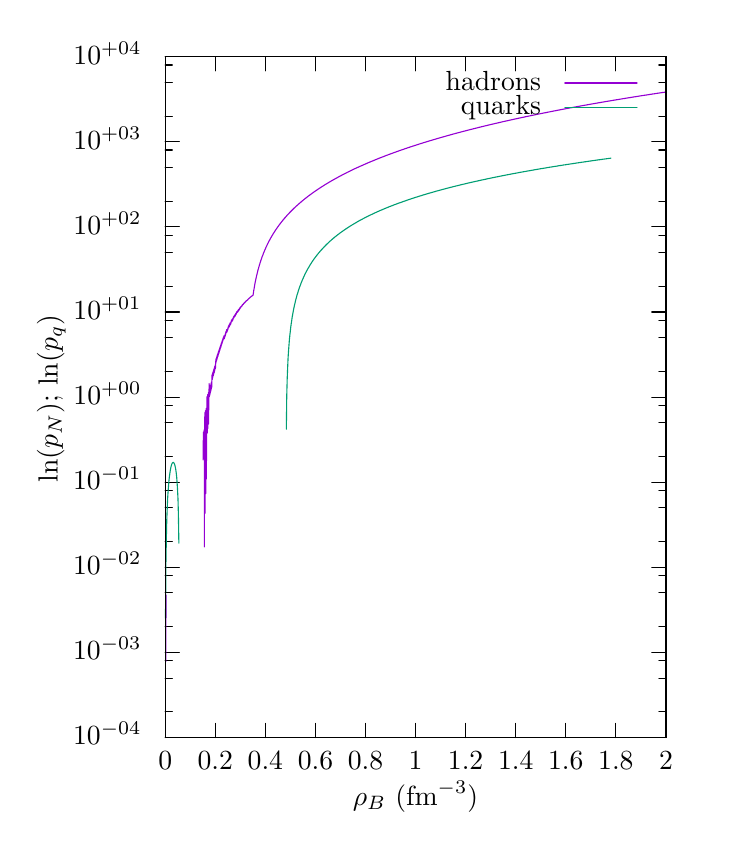
\begin{tikzpicture}[gnuplot]
%% generated with GNUPLOT 5.0p4 (Lua 5.2; terminal rev. 99, script rev. 100)
%% Thu Sep 29 16:33:14 2016
\path (0.000,0.000) rectangle (8.600,10.000);
\gpcolor{color=gp lt color border}
\gpsetlinetype{gp lt border}
\gpsetdashtype{gp dt solid}
\gpsetlinewidth{1.00}
\draw[gp path] (1.688,0.985)--(1.868,0.985);
\draw[gp path] (8.047,0.985)--(7.867,0.985);
\node[gp node right] at (1.504,0.985) {$10^{-04}$};
\draw[gp path] (1.688,1.310)--(1.778,1.310);
\draw[gp path] (8.047,1.310)--(7.957,1.310);
\draw[gp path] (1.688,1.740)--(1.778,1.740);
\draw[gp path] (8.047,1.740)--(7.957,1.740);
\draw[gp path] (1.688,1.961)--(1.778,1.961);
\draw[gp path] (8.047,1.961)--(7.957,1.961);
\draw[gp path] (1.688,2.066)--(1.868,2.066);
\draw[gp path] (8.047,2.066)--(7.867,2.066);
\node[gp node right] at (1.504,2.066) {$10^{-03}$};
\draw[gp path] (1.688,2.391)--(1.778,2.391);
\draw[gp path] (8.047,2.391)--(7.957,2.391);
\draw[gp path] (1.688,2.821)--(1.778,2.821);
\draw[gp path] (8.047,2.821)--(7.957,2.821);
\draw[gp path] (1.688,3.042)--(1.778,3.042);
\draw[gp path] (8.047,3.042)--(7.957,3.042);
\draw[gp path] (1.688,3.147)--(1.868,3.147);
\draw[gp path] (8.047,3.147)--(7.867,3.147);
\node[gp node right] at (1.504,3.147) {$10^{-02}$};
\draw[gp path] (1.688,3.472)--(1.778,3.472);
\draw[gp path] (8.047,3.472)--(7.957,3.472);
\draw[gp path] (1.688,3.902)--(1.778,3.902);
\draw[gp path] (8.047,3.902)--(7.957,3.902);
\draw[gp path] (1.688,4.123)--(1.778,4.123);
\draw[gp path] (8.047,4.123)--(7.957,4.123);
\draw[gp path] (1.688,4.227)--(1.868,4.227);
\draw[gp path] (8.047,4.227)--(7.867,4.227);
\node[gp node right] at (1.504,4.227) {$10^{-01}$};
\draw[gp path] (1.688,4.553)--(1.778,4.553);
\draw[gp path] (8.047,4.553)--(7.957,4.553);
\draw[gp path] (1.688,4.983)--(1.778,4.983);
\draw[gp path] (8.047,4.983)--(7.957,4.983);
\draw[gp path] (1.688,5.203)--(1.778,5.203);
\draw[gp path] (8.047,5.203)--(7.957,5.203);
\draw[gp path] (1.688,5.308)--(1.868,5.308);
\draw[gp path] (8.047,5.308)--(7.867,5.308);
\node[gp node right] at (1.504,5.308) {$10^{+00}$};
\draw[gp path] (1.688,5.633)--(1.778,5.633);
\draw[gp path] (8.047,5.633)--(7.957,5.633);
\draw[gp path] (1.688,6.063)--(1.778,6.063);
\draw[gp path] (8.047,6.063)--(7.957,6.063);
\draw[gp path] (1.688,6.284)--(1.778,6.284);
\draw[gp path] (8.047,6.284)--(7.957,6.284);
\draw[gp path] (1.688,6.389)--(1.868,6.389);
\draw[gp path] (8.047,6.389)--(7.867,6.389);
\node[gp node right] at (1.504,6.389) {$10^{+01}$};
\draw[gp path] (1.688,6.714)--(1.778,6.714);
\draw[gp path] (8.047,6.714)--(7.957,6.714);
\draw[gp path] (1.688,7.144)--(1.778,7.144);
\draw[gp path] (8.047,7.144)--(7.957,7.144);
\draw[gp path] (1.688,7.365)--(1.778,7.365);
\draw[gp path] (8.047,7.365)--(7.957,7.365);
\draw[gp path] (1.688,7.470)--(1.868,7.470);
\draw[gp path] (8.047,7.470)--(7.867,7.470);
\node[gp node right] at (1.504,7.470) {$10^{+02}$};
\draw[gp path] (1.688,7.795)--(1.778,7.795);
\draw[gp path] (8.047,7.795)--(7.957,7.795);
\draw[gp path] (1.688,8.225)--(1.778,8.225);
\draw[gp path] (8.047,8.225)--(7.957,8.225);
\draw[gp path] (1.688,8.446)--(1.778,8.446);
\draw[gp path] (8.047,8.446)--(7.957,8.446);
\draw[gp path] (1.688,8.550)--(1.868,8.550);
\draw[gp path] (8.047,8.550)--(7.867,8.550);
\node[gp node right] at (1.504,8.550) {$10^{+03}$};
\draw[gp path] (1.688,8.876)--(1.778,8.876);
\draw[gp path] (8.047,8.876)--(7.957,8.876);
\draw[gp path] (1.688,9.306)--(1.778,9.306);
\draw[gp path] (8.047,9.306)--(7.957,9.306);
\draw[gp path] (1.688,9.526)--(1.778,9.526);
\draw[gp path] (8.047,9.526)--(7.957,9.526);
\draw[gp path] (1.688,9.631)--(1.868,9.631);
\draw[gp path] (8.047,9.631)--(7.867,9.631);
\node[gp node right] at (1.504,9.631) {$10^{+04}$};
\draw[gp path] (1.688,0.985)--(1.688,1.165);
\draw[gp path] (1.688,9.631)--(1.688,9.451);
\node[gp node center] at (1.688,0.677) {$0$};
\draw[gp path] (2.324,0.985)--(2.324,1.165);
\draw[gp path] (2.324,9.631)--(2.324,9.451);
\node[gp node center] at (2.324,0.677) {$0.2$};
\draw[gp path] (2.960,0.985)--(2.960,1.165);
\draw[gp path] (2.960,9.631)--(2.960,9.451);
\node[gp node center] at (2.960,0.677) {$0.4$};
\draw[gp path] (3.596,0.985)--(3.596,1.165);
\draw[gp path] (3.596,9.631)--(3.596,9.451);
\node[gp node center] at (3.596,0.677) {$0.6$};
\draw[gp path] (4.232,0.985)--(4.232,1.165);
\draw[gp path] (4.232,9.631)--(4.232,9.451);
\node[gp node center] at (4.232,0.677) {$0.8$};
\draw[gp path] (4.868,0.985)--(4.868,1.165);
\draw[gp path] (4.868,9.631)--(4.868,9.451);
\node[gp node center] at (4.868,0.677) {$1$};
\draw[gp path] (5.503,0.985)--(5.503,1.165);
\draw[gp path] (5.503,9.631)--(5.503,9.451);
\node[gp node center] at (5.503,0.677) {$1.2$};
\draw[gp path] (6.139,0.985)--(6.139,1.165);
\draw[gp path] (6.139,9.631)--(6.139,9.451);
\node[gp node center] at (6.139,0.677) {$1.4$};
\draw[gp path] (6.775,0.985)--(6.775,1.165);
\draw[gp path] (6.775,9.631)--(6.775,9.451);
\node[gp node center] at (6.775,0.677) {$1.6$};
\draw[gp path] (7.411,0.985)--(7.411,1.165);
\draw[gp path] (7.411,9.631)--(7.411,9.451);
\node[gp node center] at (7.411,0.677) {$1.8$};
\draw[gp path] (8.047,0.985)--(8.047,1.165);
\draw[gp path] (8.047,9.631)--(8.047,9.451);
\node[gp node center] at (8.047,0.677) {$2$};
\draw[gp path] (1.688,9.631)--(1.688,0.985)--(8.047,0.985)--(8.047,9.631)--cycle;
\node[gp node center,rotate=-270] at (0.246,5.308) {$\ln(p_N)$; $\ln(p_q)$};
\node[gp node center] at (4.867,0.215) {$\rho_B$ ($\rm{fm}^{-3}$)};
\node[gp node right] at (6.579,9.297) {hadrons};
\gpcolor{rgb color={0.580,0.000,0.827}}
\draw[gp path] (6.763,9.297)--(7.679,9.297);
\draw[gp path] (1.695,1.949)--(1.698,2.796);
\draw[gp path] (2.170,4.510)--(2.172,4.863);
\draw[gp path] (2.179,4.561)--(2.181,4.893);
\draw[gp path] (2.185,3.406)--(2.187,4.616)--(2.189,4.925)--(2.191,5.111)--(2.193,3.832)%
  --(2.196,4.673)--(2.198,4.959)--(2.200,5.137)--(2.202,4.083)--(2.204,4.732)--(2.206,4.996)%
  --(2.208,5.165)--(2.210,4.268)--(2.213,4.792)--(2.215,5.034)--(2.217,5.195)--(2.219,5.315)%
  --(2.221,4.851)--(2.223,5.074)--(2.225,5.225)--(2.227,5.340)--(2.229,4.909)--(2.232,5.114)%
  --(2.234,5.257)--(2.236,5.367)--(2.238,4.967)--(2.240,5.155)--(2.242,5.289)--(2.244,5.394)%
  --(2.246,5.481)--(2.249,5.314)--(2.251,5.415)--(2.253,5.331)--(2.255,5.430)--(2.257,5.347)%
  --(2.259,5.444)--(2.261,5.364)--(2.263,5.458)--(2.266,5.381)--(2.268,5.473)--(2.270,5.398)%
  --(2.272,5.488)--(2.274,5.415)--(2.276,5.502)--(2.278,5.432)--(2.280,5.517)--(2.282,5.589)%
  --(2.285,5.532)--(2.287,5.603)--(2.289,5.547)--(2.291,5.616)--(2.293,5.562)--(2.295,5.629)%
  --(2.297,5.577)--(2.299,5.643)--(2.302,5.591)--(2.304,5.656)--(2.306,5.606)--(2.308,5.670)%
  --(2.310,5.621)--(2.312,5.683)--(2.314,5.636)--(2.316,5.697)--(2.318,5.651)--(2.321,5.710)%
  --(2.323,5.666)--(2.325,5.724)--(2.327,5.681)--(2.329,5.738)--(2.331,5.788)--(2.333,5.751)%
  --(2.335,5.801)--(2.338,5.765)--(2.340,5.814)--(2.342,5.778)--(2.344,5.826)--(2.346,5.792)%
  --(2.348,5.839)--(2.350,5.805)--(2.352,5.851)--(2.355,5.819)--(2.357,5.864)--(2.359,5.832)%
  --(2.361,5.876)--(2.363,5.846)--(2.365,5.889)--(2.367,5.859)--(2.369,5.901)--(2.371,5.872)%
  --(2.374,5.914)--(2.376,5.886)--(2.378,5.926)--(2.380,5.899)--(2.382,5.939)--(2.384,5.912)%
  --(2.386,5.951)--(2.388,5.925)--(2.391,5.964)--(2.393,5.939)--(2.395,5.976)--(2.397,5.952)%
  --(2.399,5.988)--(2.401,5.965)--(2.403,6.001)--(2.405,5.978)--(2.408,6.013)--(2.410,5.991)%
  --(2.412,6.025)--(2.414,6.004)--(2.416,6.037)--(2.418,6.016)--(2.420,6.050)--(2.422,6.029)%
  --(2.424,6.062)--(2.427,6.042)--(2.429,6.074)--(2.431,6.054)--(2.433,6.086)--(2.435,6.067)%
  --(2.437,6.048)--(2.439,6.080)--(2.441,6.061)--(2.444,6.092)--(2.446,6.074)--(2.448,6.104)%
  --(2.450,6.087)--(2.452,6.117)--(2.454,6.100)--(2.456,6.129)--(2.458,6.112)--(2.460,6.141)%
  --(2.463,6.125)--(2.465,6.153)--(2.467,6.138)--(2.469,6.166)--(2.471,6.150)--(2.473,6.135)%
  --(2.475,6.163)--(2.477,6.148)--(2.480,6.175)--(2.482,6.161)--(2.484,6.188)--(2.486,6.174)%
  --(2.488,6.200)--(2.490,6.186)--(2.492,6.212)--(2.494,6.199)--(2.497,6.224)--(2.499,6.212)%
  --(2.501,6.199)--(2.503,6.224)--(2.505,6.212)--(2.507,6.236)--(2.509,6.224)--(2.511,6.249)%
  --(2.513,6.237)--(2.516,6.225)--(2.518,6.250)--(2.520,6.238)--(2.522,6.262)--(2.524,6.251)%
  --(2.526,6.275)--(2.528,6.264)--(2.530,6.287)--(2.533,6.277)--(2.535,6.266)--(2.537,6.289)%
  --(2.539,6.279)--(2.541,6.302)--(2.543,6.292)--(2.545,6.282)--(2.547,6.305)--(2.550,6.296)%
  --(2.552,6.318)--(2.554,6.309)--(2.556,6.330)--(2.558,6.322)--(2.560,6.313)--(2.562,6.335)%
  --(2.564,6.326)--(2.566,6.347)--(2.569,6.339)--(2.571,6.331)--(2.573,6.352)--(2.575,6.344)%
  --(2.577,6.337)--(2.579,6.358)--(2.581,6.350)--(2.583,6.371)--(2.586,6.363)--(2.588,6.356)%
  --(2.590,6.377)--(2.592,6.370)--(2.594,6.390)--(2.596,6.383)--(2.598,6.377)--(2.600,6.397)%
  --(2.602,6.390)--(2.605,6.384)--(2.607,6.404)--(2.609,6.398)--(2.611,6.392)--(2.613,6.412)%
  --(2.615,6.406)--(2.617,6.401)--(2.619,6.420)--(2.622,6.415)--(2.624,6.410)--(2.626,6.429)%
  --(2.628,6.424)--(2.630,6.419)--(2.632,6.438)--(2.634,6.434)--(2.636,6.429)--(2.639,6.448)%
  --(2.641,6.438)--(2.643,6.445)--(2.645,6.452)--(2.647,6.449)--(2.649,6.456)--(2.651,6.452)%
  --(2.653,6.460)--(2.655,6.456)--(2.658,6.464)--(2.660,6.461)--(2.662,6.468)--(2.664,6.476)%
  --(2.666,6.473)--(2.668,6.481)--(2.670,6.478)--(2.672,6.486)--(2.675,6.484)--(2.677,6.482)%
  --(2.679,6.489)--(2.681,6.488)--(2.683,6.496)--(2.685,6.494)--(2.687,6.502)--(2.689,6.501)%
  --(2.691,6.500)--(2.694,6.508)--(2.696,6.507)--(2.698,6.506)--(2.700,6.514)--(2.702,6.514)%
  --(2.704,6.514)--(2.706,6.522)--(2.708,6.522)--(2.711,6.522)--(2.713,6.522)--(2.715,6.531)%
  --(2.717,6.532)--(2.719,6.532)--(2.721,6.533)--(2.723,6.534)--(2.725,6.536)--(2.728,6.537)%
  --(2.730,6.539)--(2.732,6.541)--(2.734,6.543)--(2.736,6.545)--(2.738,6.547)--(2.740,6.550)%
  --(2.742,6.552)--(2.744,6.555)--(2.747,6.558)--(2.749,6.561)--(2.751,6.559)--(2.753,6.562)%
  --(2.755,6.566)--(2.757,6.565)--(2.759,6.569)--(2.761,6.569)--(2.764,6.571)--(2.766,6.574)%
  --(2.768,6.577)--(2.770,6.577)--(2.772,6.578)--(2.774,6.580)--(2.776,6.582)--(2.778,6.584)%
  --(2.781,6.585)--(2.783,6.588)--(2.785,6.588)--(2.787,6.591)--(2.789,6.591)--(2.791,6.594)%
  --(2.793,6.595)--(2.795,6.597)--(2.797,6.598)--(2.800,6.600)--(2.802,6.601)--(2.804,6.605)%
  --(2.806,6.620)--(2.808,6.634)--(2.810,6.648)--(2.812,6.662)--(2.814,6.675)--(2.817,6.688)%
  --(2.819,6.700)--(2.821,6.712)--(2.823,6.724)--(2.825,6.736)--(2.827,6.747)--(2.829,6.759)%
  --(2.831,6.769)--(2.833,6.780)--(2.836,6.791)--(2.838,6.801)--(2.840,6.811)--(2.842,6.821)%
  --(2.844,6.830)--(2.846,6.840)--(2.848,6.849)--(2.850,6.858)--(2.853,6.867)--(2.855,6.876)%
  --(2.857,6.885)--(2.859,6.893)--(2.861,6.902)--(2.863,6.910)--(2.865,6.918)--(2.867,6.926)%
  --(2.870,6.934)--(2.872,6.942)--(2.874,6.949)--(2.876,6.957)--(2.878,6.964)--(2.880,6.971)%
  --(2.882,6.979)--(2.884,6.986)--(2.886,6.993)--(2.889,7.000)--(2.891,7.007)--(2.893,7.013)%
  --(2.895,7.020)--(2.897,7.027)--(2.899,7.033)--(2.901,7.040)--(2.903,7.046)--(2.906,7.052)%
  --(2.908,7.058)--(2.910,7.065)--(2.912,7.071)--(2.914,7.077)--(2.916,7.083)--(2.918,7.088)%
  --(2.920,7.094)--(2.923,7.100)--(2.925,7.106)--(2.927,7.111)--(2.929,7.117)--(2.931,7.122)%
  --(2.933,7.128)--(2.935,7.133)--(2.937,7.139)--(2.939,7.144)--(2.942,7.149)--(2.944,7.154)%
  --(2.946,7.159)--(2.948,7.164)--(2.950,7.170)--(2.952,7.175)--(2.954,7.179)--(2.956,7.184)%
  --(2.959,7.189)--(2.961,7.194)--(2.963,7.199)--(2.965,7.204)--(2.967,7.208)--(2.969,7.213)%
  --(2.971,7.218)--(2.973,7.222)--(2.975,7.227)--(2.978,7.231)--(2.980,7.236)--(2.982,7.240)%
  --(2.984,7.245)--(2.986,7.249)--(2.988,7.253)--(2.990,7.258)--(2.992,7.262)--(2.995,7.266)%
  --(2.997,7.270)--(2.999,7.274)--(3.001,7.279)--(3.003,7.283)--(3.005,7.287)--(3.007,7.291)%
  --(3.009,7.295)--(3.012,7.299)--(3.014,7.303)--(3.016,7.307)--(3.018,7.311)--(3.020,7.315)%
  --(3.022,7.318)--(3.024,7.322)--(3.026,7.326)--(3.028,7.330)--(3.031,7.334)--(3.033,7.337)%
  --(3.035,7.341)--(3.037,7.345)--(3.039,7.348)--(3.041,7.352)--(3.043,7.356)--(3.045,7.359)%
  --(3.048,7.363)--(3.050,7.366)--(3.052,7.370)--(3.054,7.373)--(3.056,7.377)--(3.058,7.380)%
  --(3.060,7.384)--(3.062,7.387)--(3.064,7.391)--(3.067,7.394)--(3.069,7.397)--(3.071,7.401)%
  --(3.073,7.404)--(3.075,7.407)--(3.077,7.411)--(3.079,7.414)--(3.081,7.417)--(3.084,7.420)%
  --(3.086,7.424)--(3.088,7.427)--(3.090,7.430)--(3.092,7.433)--(3.094,7.436)--(3.096,7.439)%
  --(3.098,7.442)--(3.101,7.446)--(3.103,7.449)--(3.105,7.452)--(3.107,7.455)--(3.109,7.458)%
  --(3.111,7.461)--(3.113,7.464)--(3.115,7.467)--(3.117,7.470)--(3.120,7.473)--(3.122,7.476)%
  --(3.124,7.479)--(3.126,7.482)--(3.128,7.484)--(3.130,7.487)--(3.132,7.490)--(3.134,7.493)%
  --(3.137,7.496)--(3.139,7.499)--(3.141,7.502)--(3.143,7.504)--(3.145,7.507)--(3.147,7.510)%
  --(3.149,7.513)--(3.151,7.515)--(3.154,7.518)--(3.156,7.521)--(3.158,7.524)--(3.160,7.526)%
  --(3.162,7.529)--(3.164,7.532)--(3.166,7.534)--(3.168,7.537)--(3.170,7.540)--(3.173,7.542)%
  --(3.175,7.545)--(3.177,7.548)--(3.179,7.550)--(3.181,7.553)--(3.183,7.555)--(3.185,7.558)%
  --(3.187,7.561)--(3.190,7.563)--(3.192,7.566)--(3.194,7.568)--(3.196,7.571)--(3.198,7.573)%
  --(3.200,7.576)--(3.202,7.578)--(3.204,7.581)--(3.206,7.583)--(3.209,7.586)--(3.211,7.588)%
  --(3.213,7.590)--(3.215,7.593)--(3.217,7.595)--(3.219,7.598)--(3.221,7.600)--(3.223,7.602)%
  --(3.226,7.605)--(3.228,7.607)--(3.230,7.610)--(3.232,7.612)--(3.234,7.614)--(3.236,7.617)%
  --(3.238,7.619)--(3.240,7.621)--(3.243,7.624)--(3.245,7.626)--(3.247,7.628)--(3.249,7.630)%
  --(3.251,7.633)--(3.253,7.635)--(3.255,7.637)--(3.257,7.640)--(3.259,7.642)--(3.262,7.644)%
  --(3.264,7.646)--(3.266,7.648)--(3.268,7.651)--(3.270,7.653)--(3.272,7.655)--(3.274,7.657)%
  --(3.276,7.659)--(3.279,7.662)--(3.281,7.664)--(3.283,7.666)--(3.285,7.668)--(3.287,7.670)%
  --(3.289,7.672)--(3.291,7.675)--(3.293,7.677)--(3.295,7.679)--(3.298,7.681)--(3.300,7.683)%
  --(3.302,7.685)--(3.304,7.687)--(3.306,7.689)--(3.308,7.691)--(3.310,7.693)--(3.312,7.696)%
  --(3.315,7.698)--(3.317,7.700)--(3.319,7.702)--(3.321,7.704)--(3.323,7.706)--(3.325,7.708)%
  --(3.327,7.710)--(3.329,7.712)--(3.332,7.714)--(3.334,7.716)--(3.336,7.718)--(3.338,7.720)%
  --(3.340,7.722)--(3.342,7.724)--(3.344,7.726)--(3.346,7.728)--(3.348,7.730)--(3.351,7.732)%
  --(3.353,7.734)--(3.355,7.736)--(3.357,7.737)--(3.359,7.739)--(3.361,7.741)--(3.363,7.743)%
  --(3.365,7.745)--(3.368,7.747)--(3.370,7.749)--(3.372,7.751)--(3.374,7.753)--(3.376,7.755)%
  --(3.378,7.756)--(3.380,7.758)--(3.382,7.760)--(3.385,7.762)--(3.387,7.764)--(3.389,7.766)%
  --(3.391,7.768)--(3.393,7.770)--(3.395,7.771)--(3.397,7.773)--(3.399,7.775)--(3.401,7.777)%
  --(3.404,7.779)--(3.406,7.780)--(3.408,7.782)--(3.410,7.784)--(3.412,7.786)--(3.414,7.788)%
  --(3.416,7.789)--(3.418,7.791)--(3.421,7.793)--(3.423,7.795)--(3.425,7.797)--(3.427,7.798)%
  --(3.429,7.800)--(3.431,7.802)--(3.433,7.804)--(3.435,7.805)--(3.437,7.807)--(3.440,7.809)%
  --(3.442,7.811)--(3.444,7.812)--(3.446,7.814)--(3.448,7.816)--(3.450,7.817)--(3.452,7.819)%
  --(3.454,7.821)--(3.457,7.823)--(3.459,7.824)--(3.461,7.826)--(3.463,7.828)--(3.465,7.829)%
  --(3.467,7.831)--(3.469,7.833)--(3.471,7.834)--(3.474,7.836)--(3.476,7.838)--(3.478,7.839)%
  --(3.480,7.841)--(3.482,7.843)--(3.484,7.844)--(3.486,7.846)--(3.488,7.848)--(3.490,7.849)%
  --(3.493,7.851)--(3.495,7.853)--(3.497,7.854)--(3.499,7.856)--(3.501,7.857)--(3.503,7.859)%
  --(3.505,7.861)--(3.507,7.862)--(3.510,7.864)--(3.512,7.865)--(3.514,7.867)--(3.516,7.869)%
  --(3.518,7.870)--(3.520,7.872)--(3.522,7.873)--(3.524,7.875)--(3.527,7.877)--(3.529,7.878)%
  --(3.531,7.880)--(3.533,7.881)--(3.535,7.883)--(3.537,7.884)--(3.539,7.886)--(3.541,7.887)%
  --(3.543,7.889)--(3.546,7.891)--(3.548,7.892)--(3.550,7.894)--(3.552,7.895)--(3.554,7.897)%
  --(3.556,7.898)--(3.558,7.900)--(3.560,7.901)--(3.563,7.903)--(3.565,7.904)--(3.567,7.906)%
  --(3.569,7.907)--(3.571,7.909)--(3.573,7.910)--(3.575,7.912)--(3.577,7.913)--(3.579,7.915)%
  --(3.582,7.916)--(3.584,7.918)--(3.586,7.919)--(3.588,7.921)--(3.590,7.922)--(3.592,7.924)%
  --(3.594,7.925)--(3.596,7.927)--(3.599,7.928)--(3.601,7.929)--(3.603,7.931)--(3.605,7.932)%
  --(3.607,7.934)--(3.609,7.935)--(3.611,7.937)--(3.613,7.938)--(3.616,7.940)--(3.618,7.941)%
  --(3.620,7.942)--(3.622,7.944)--(3.624,7.945)--(3.626,7.947)--(3.628,7.948)--(3.630,7.950)%
  --(3.632,7.951)--(3.635,7.952)--(3.637,7.954)--(3.639,7.955)--(3.641,7.957)--(3.643,7.958)%
  --(3.645,7.959)--(3.647,7.961)--(3.649,7.962)--(3.652,7.964)--(3.654,7.965)--(3.656,7.966)%
  --(3.658,7.968)--(3.660,7.969)--(3.662,7.970)--(3.664,7.972)--(3.666,7.973)--(3.668,7.975)%
  --(3.671,7.976)--(3.673,7.977)--(3.675,7.979)--(3.677,7.980)--(3.679,7.981)--(3.681,7.983)%
  --(3.683,7.984)--(3.685,7.985)--(3.688,7.987)--(3.690,7.988)--(3.692,7.989)--(3.694,7.991)%
  --(3.696,7.992)--(3.698,7.993)--(3.700,7.995)--(3.702,7.996)--(3.705,7.997)--(3.707,7.999)%
  --(3.709,8.000)--(3.711,8.001)--(3.713,8.003)--(3.715,8.004)--(3.717,8.005)--(3.719,8.007)%
  --(3.721,8.008)--(3.724,8.009)--(3.726,8.011)--(3.728,8.012)--(3.730,8.013)--(3.732,8.014)%
  --(3.734,8.016)--(3.736,8.017)--(3.738,8.018)--(3.741,8.020)--(3.743,8.021)--(3.745,8.022)%
  --(3.747,8.023)--(3.749,8.025)--(3.751,8.026)--(3.753,8.027)--(3.755,8.029)--(3.758,8.030)%
  --(3.760,8.031)--(3.762,8.032)--(3.764,8.034)--(3.766,8.035)--(3.768,8.036)--(3.770,8.037)%
  --(3.772,8.039)--(3.774,8.040)--(3.777,8.041)--(3.779,8.042)--(3.781,8.044)--(3.783,8.045)%
  --(3.785,8.046)--(3.787,8.047)--(3.789,8.049)--(3.791,8.050)--(3.794,8.051)--(3.796,8.052)%
  --(3.798,8.053)--(3.800,8.055)--(3.802,8.056)--(3.804,8.057)--(3.806,8.058)--(3.808,8.060)%
  --(3.810,8.061)--(3.813,8.062)--(3.815,8.063)--(3.817,8.064)--(3.819,8.066)--(3.821,8.067)%
  --(3.823,8.068)--(3.825,8.069)--(3.827,8.070)--(3.830,8.072)--(3.832,8.073)--(3.834,8.074)%
  --(3.836,8.075)--(3.838,8.076)--(3.840,8.078)--(3.842,8.079)--(3.844,8.080)--(3.847,8.081)%
  --(3.849,8.082)--(3.851,8.083)--(3.853,8.085)--(3.855,8.086)--(3.857,8.087)--(3.859,8.088)%
  --(3.861,8.089)--(3.863,8.090)--(3.866,8.092)--(3.868,8.093)--(3.870,8.094)--(3.872,8.095)%
  --(3.874,8.096)--(3.876,8.097)--(3.878,8.099)--(3.880,8.100)--(3.883,8.101)--(3.885,8.102)%
  --(3.887,8.103)--(3.889,8.104)--(3.891,8.105)--(3.893,8.107)--(3.895,8.108)--(3.897,8.109)%
  --(3.900,8.110)--(3.902,8.111)--(3.904,8.112)--(3.906,8.113)--(3.908,8.115)--(3.910,8.116)%
  --(3.912,8.117)--(3.914,8.118)--(3.916,8.119)--(3.919,8.120)--(3.921,8.121)--(3.923,8.122)%
  --(3.925,8.124)--(3.927,8.125)--(3.929,8.126)--(3.931,8.127)--(3.933,8.128)--(3.936,8.129)%
  --(3.938,8.130)--(3.940,8.131)--(3.942,8.132)--(3.944,8.133)--(3.946,8.135)--(3.948,8.136)%
  --(3.950,8.137)--(3.952,8.138)--(3.955,8.139)--(3.957,8.140)--(3.959,8.141)--(3.961,8.142)%
  --(3.963,8.143)--(3.965,8.144)--(3.967,8.145)--(3.969,8.147)--(3.972,8.148)--(3.974,8.149)%
  --(3.976,8.150)--(3.978,8.151)--(3.980,8.152)--(3.982,8.153)--(3.984,8.154)--(3.986,8.155)%
  --(3.989,8.156)--(3.991,8.157)--(3.993,8.158)--(3.995,8.159)--(3.997,8.160)--(3.999,8.162)%
  --(4.001,8.163)--(4.003,8.164)--(4.005,8.165)--(4.008,8.166)--(4.010,8.167)--(4.012,8.168)%
  --(4.014,8.169)--(4.016,8.170)--(4.018,8.171)--(4.020,8.172)--(4.022,8.173)--(4.025,8.174)%
  --(4.027,8.175)--(4.029,8.176)--(4.031,8.177)--(4.033,8.178)--(4.035,8.179)--(4.037,8.180)%
  --(4.039,8.181)--(4.041,8.182)--(4.044,8.183)--(4.046,8.184)--(4.048,8.186)--(4.050,8.187)%
  --(4.052,8.188)--(4.054,8.189)--(4.056,8.190)--(4.058,8.191)--(4.061,8.192)--(4.063,8.193)%
  --(4.065,8.194)--(4.067,8.195)--(4.069,8.196)--(4.071,8.197)--(4.073,8.198)--(4.075,8.199)%
  --(4.078,8.200)--(4.080,8.201)--(4.082,8.202)--(4.084,8.203)--(4.086,8.204)--(4.088,8.205)%
  --(4.090,8.206)--(4.092,8.207)--(4.094,8.208)--(4.097,8.209)--(4.099,8.210)--(4.101,8.211)%
  --(4.103,8.212)--(4.105,8.213)--(4.107,8.214)--(4.109,8.215)--(4.111,8.216)--(4.114,8.217)%
  --(4.116,8.218)--(4.118,8.219)--(4.120,8.220)--(4.122,8.221)--(4.124,8.222)--(4.126,8.223)%
  --(4.128,8.224)--(4.131,8.225)--(4.133,8.225)--(4.135,8.226)--(4.137,8.227)--(4.139,8.228)%
  --(4.141,8.229)--(4.143,8.230)--(4.145,8.231)--(4.147,8.232)--(4.150,8.233)--(4.152,8.234)%
  --(4.154,8.235)--(4.156,8.236)--(4.158,8.237)--(4.160,8.238)--(4.162,8.239)--(4.164,8.240)%
  --(4.167,8.241)--(4.169,8.242)--(4.171,8.243)--(4.173,8.244)--(4.175,8.245)--(4.177,8.246)%
  --(4.179,8.247)--(4.181,8.248)--(4.183,8.249)--(4.186,8.249)--(4.188,8.250)--(4.190,8.251)%
  --(4.192,8.252)--(4.194,8.253)--(4.196,8.254)--(4.198,8.255)--(4.200,8.256)--(4.203,8.257)%
  --(4.205,8.258)--(4.207,8.259)--(4.209,8.260)--(4.211,8.261)--(4.213,8.262)--(4.215,8.263)%
  --(4.217,8.264)--(4.220,8.264)--(4.222,8.265)--(4.224,8.266)--(4.226,8.267)--(4.228,8.268)%
  --(4.230,8.269)--(4.232,8.270)--(4.234,8.271)--(4.236,8.272)--(4.239,8.273)--(4.241,8.274)%
  --(4.243,8.275)--(4.245,8.275)--(4.247,8.276)--(4.249,8.277)--(4.251,8.278)--(4.253,8.279)%
  --(4.256,8.280)--(4.258,8.281)--(4.260,8.282)--(4.262,8.283)--(4.264,8.284)--(4.266,8.285)%
  --(4.268,8.285)--(4.270,8.286)--(4.273,8.287)--(4.275,8.288)--(4.277,8.289)--(4.279,8.290)%
  --(4.281,8.291)--(4.283,8.292)--(4.285,8.293)--(4.287,8.294)--(4.289,8.294)--(4.292,8.295)%
  --(4.294,8.296)--(4.296,8.297)--(4.298,8.298)--(4.300,8.299)--(4.302,8.300)--(4.304,8.301)%
  --(4.306,8.302)--(4.309,8.302)--(4.311,8.303)--(4.313,8.304)--(4.315,8.305)--(4.317,8.306)%
  --(4.319,8.307)--(4.321,8.308)--(4.323,8.309)--(4.325,8.309)--(4.328,8.310)--(4.330,8.311)%
  --(4.332,8.312)--(4.334,8.313)--(4.336,8.314)--(4.338,8.315)--(4.340,8.316)--(4.342,8.316)%
  --(4.345,8.317)--(4.347,8.318)--(4.349,8.319)--(4.351,8.320)--(4.353,8.321)--(4.355,8.322)%
  --(4.357,8.322)--(4.359,8.323)--(4.362,8.324)--(4.364,8.325)--(4.366,8.326)--(4.368,8.327)%
  --(4.370,8.328)--(4.372,8.328)--(4.374,8.329)--(4.376,8.330)--(4.378,8.331)--(4.381,8.332)%
  --(4.383,8.333)--(4.385,8.334)--(4.387,8.334)--(4.389,8.335)--(4.391,8.336)--(4.393,8.337)%
  --(4.395,8.338)--(4.398,8.339)--(4.400,8.339)--(4.402,8.340)--(4.404,8.341)--(4.406,8.342)%
  --(4.408,8.343)--(4.410,8.344)--(4.412,8.345)--(4.414,8.345)--(4.417,8.346)--(4.419,8.347)%
  --(4.421,8.348)--(4.423,8.349)--(4.425,8.350)--(4.427,8.350)--(4.429,8.351)--(4.431,8.352)%
  --(4.434,8.353)--(4.436,8.354)--(4.438,8.355)--(4.440,8.355)--(4.442,8.356)--(4.444,8.357)%
  --(4.446,8.358)--(4.448,8.359)--(4.451,8.359)--(4.453,8.360)--(4.455,8.361)--(4.457,8.362)%
  --(4.459,8.363)--(4.461,8.364)--(4.463,8.364)--(4.465,8.365)--(4.467,8.366)--(4.470,8.367)%
  --(4.472,8.368)--(4.474,8.368)--(4.476,8.369)--(4.478,8.370)--(4.480,8.371)--(4.482,8.372)%
  --(4.484,8.372)--(4.487,8.373)--(4.489,8.374)--(4.491,8.375)--(4.493,8.376)--(4.495,8.377)%
  --(4.497,8.377)--(4.499,8.378)--(4.501,8.379)--(4.504,8.380)--(4.506,8.381)--(4.508,8.381)%
  --(4.510,8.382)--(4.512,8.383)--(4.514,8.384)--(4.516,8.385)--(4.518,8.385)--(4.520,8.386)%
  --(4.523,8.387)--(4.525,8.388)--(4.527,8.388)--(4.529,8.389)--(4.531,8.390)--(4.533,8.391)%
  --(4.535,8.392)--(4.537,8.392)--(4.540,8.393)--(4.542,8.394)--(4.544,8.395)--(4.546,8.396)%
  --(4.548,8.396)--(4.550,8.397)--(4.552,8.398)--(4.554,8.399)--(4.556,8.400)--(4.559,8.400)%
  --(4.561,8.401)--(4.563,8.402)--(4.565,8.403)--(4.567,8.403)--(4.569,8.404)--(4.571,8.405)%
  --(4.573,8.406)--(4.576,8.407)--(4.578,8.407)--(4.580,8.408)--(4.582,8.409)--(4.584,8.410)%
  --(4.586,8.410)--(4.588,8.411)--(4.590,8.412)--(4.593,8.413)--(4.595,8.413)--(4.597,8.414)%
  --(4.599,8.415)--(4.601,8.416)--(4.603,8.417)--(4.605,8.417)--(4.607,8.418)--(4.609,8.419)%
  --(4.612,8.420)--(4.614,8.420)--(4.616,8.421)--(4.618,8.422)--(4.620,8.423)--(4.622,8.423)%
  --(4.624,8.424)--(4.626,8.425)--(4.629,8.426)--(4.631,8.426)--(4.633,8.427)--(4.635,8.428)%
  --(4.637,8.429)--(4.639,8.429)--(4.641,8.430)--(4.643,8.431)--(4.646,8.432)--(4.648,8.432)%
  --(4.650,8.433)--(4.652,8.434)--(4.654,8.435)--(4.656,8.435)--(4.658,8.436)--(4.660,8.437)%
  --(4.662,8.438)--(4.665,8.438)--(4.667,8.439)--(4.669,8.440)--(4.671,8.441)--(4.673,8.441)%
  --(4.675,8.442)--(4.677,8.443)--(4.679,8.444)--(4.682,8.444)--(4.684,8.445)--(4.686,8.446)%
  --(4.688,8.447)--(4.690,8.447)--(4.692,8.448)--(4.694,8.449)--(4.696,8.450)--(4.698,8.450)%
  --(4.701,8.451)--(4.703,8.452)--(4.705,8.452)--(4.707,8.453)--(4.709,8.454)--(4.711,8.455)%
  --(4.713,8.455)--(4.715,8.456)--(4.718,8.457)--(4.720,8.458)--(4.722,8.458)--(4.724,8.459)%
  --(4.726,8.460)--(4.728,8.460)--(4.730,8.461)--(4.732,8.462)--(4.735,8.463)--(4.737,8.463)%
  --(4.739,8.464)--(4.741,8.465)--(4.743,8.466)--(4.745,8.466)--(4.747,8.467)--(4.749,8.468)%
  --(4.751,8.468)--(4.754,8.469)--(4.756,8.470)--(4.758,8.471)--(4.760,8.471)--(4.762,8.472)%
  --(4.764,8.473)--(4.766,8.473)--(4.768,8.474)--(4.771,8.475)--(4.773,8.476)--(4.775,8.476)%
  --(4.777,8.477)--(4.779,8.478)--(4.781,8.478)--(4.783,8.479)--(4.785,8.480)--(4.787,8.481)%
  --(4.790,8.481)--(4.792,8.482)--(4.794,8.483)--(4.796,8.483)--(4.798,8.484)--(4.800,8.485)%
  --(4.802,8.485)--(4.804,8.486)--(4.807,8.487)--(4.809,8.488)--(4.811,8.488)--(4.813,8.489)%
  --(4.815,8.490)--(4.817,8.490)--(4.819,8.491)--(4.821,8.492)--(4.824,8.492)--(4.826,8.493)%
  --(4.828,8.494)--(4.830,8.495)--(4.832,8.495)--(4.834,8.496)--(4.836,8.497)--(4.838,8.497)%
  --(4.840,8.498)--(4.843,8.499)--(4.845,8.499)--(4.847,8.500)--(4.849,8.501)--(4.851,8.501)%
  --(4.853,8.502)--(4.855,8.503)--(4.857,8.504)--(4.860,8.504)--(4.862,8.505)--(4.864,8.506)%
  --(4.866,8.506)--(4.868,8.507)--(4.870,8.508)--(4.872,8.508)--(4.874,8.509)--(4.877,8.510)%
  --(4.879,8.510)--(4.881,8.511)--(4.883,8.512)--(4.885,8.512)--(4.887,8.513)--(4.889,8.514)%
  --(4.891,8.514)--(4.893,8.515)--(4.896,8.516)--(4.898,8.516)--(4.900,8.517)--(4.902,8.518)%
  --(4.904,8.519)--(4.906,8.519)--(4.908,8.520)--(4.910,8.521)--(4.913,8.521)--(4.915,8.522)%
  --(4.917,8.523)--(4.919,8.523)--(4.921,8.524)--(4.923,8.525)--(4.925,8.525)--(4.927,8.526)%
  --(4.929,8.527)--(4.932,8.527)--(4.934,8.528)--(4.936,8.529)--(4.938,8.529)--(4.940,8.530)%
  --(4.942,8.531)--(4.944,8.531)--(4.946,8.532)--(4.949,8.533)--(4.951,8.533)--(4.953,8.534)%
  --(4.955,8.535)--(4.957,8.535)--(4.959,8.536)--(4.961,8.537)--(4.963,8.537)--(4.966,8.538)%
  --(4.968,8.539)--(4.970,8.539)--(4.972,8.540)--(4.974,8.541)--(4.976,8.541)--(4.978,8.542)%
  --(4.980,8.543)--(4.982,8.543)--(4.985,8.544)--(4.987,8.544)--(4.989,8.545)--(4.991,8.546)%
  --(4.993,8.546)--(4.995,8.547)--(4.997,8.548)--(4.999,8.548)--(5.002,8.549)--(5.004,8.550)%
  --(5.006,8.550)--(5.008,8.551)--(5.010,8.552)--(5.012,8.552)--(5.014,8.553)--(5.016,8.554)%
  --(5.019,8.554)--(5.021,8.555)--(5.023,8.556)--(5.025,8.556)--(5.027,8.557)--(5.029,8.557)%
  --(5.031,8.558)--(5.033,8.559)--(5.035,8.559)--(5.038,8.560)--(5.040,8.561)--(5.042,8.561)%
  --(5.044,8.562)--(5.046,8.563)--(5.048,8.563)--(5.050,8.564)--(5.052,8.565)--(5.055,8.565)%
  --(5.057,8.566)--(5.059,8.566)--(5.061,8.567)--(5.063,8.568)--(5.065,8.568)--(5.067,8.569)%
  --(5.069,8.570)--(5.071,8.570)--(5.074,8.571)--(5.076,8.572)--(5.078,8.572)--(5.080,8.573)%
  --(5.082,8.573)--(5.084,8.574)--(5.086,8.575)--(5.088,8.575)--(5.091,8.576)--(5.093,8.577)%
  --(5.095,8.577)--(5.097,8.578)--(5.099,8.578)--(5.101,8.579)--(5.103,8.580)--(5.105,8.580)%
  --(5.108,8.581)--(5.110,8.582)--(5.112,8.582)--(5.114,8.583)--(5.116,8.583)--(5.118,8.584)%
  --(5.120,8.585)--(5.122,8.585)--(5.124,8.586)--(5.127,8.587)--(5.129,8.587)--(5.131,8.588)%
  --(5.133,8.588)--(5.135,8.589)--(5.137,8.590)--(5.139,8.590)--(5.141,8.591)--(5.144,8.592)%
  --(5.146,8.592)--(5.148,8.593)--(5.150,8.593)--(5.152,8.594)--(5.154,8.595)--(5.156,8.595)%
  --(5.158,8.596)--(5.160,8.597)--(5.163,8.597)--(5.165,8.598)--(5.167,8.598)--(5.169,8.599)%
  --(5.171,8.600)--(5.173,8.600)--(5.175,8.601)--(5.177,8.601)--(5.180,8.602)--(5.182,8.603)%
  --(5.184,8.603)--(5.186,8.604)--(5.188,8.604)--(5.190,8.605)--(5.192,8.606)--(5.194,8.606)%
  --(5.197,8.607)--(5.199,8.608)--(5.201,8.608)--(5.203,8.609)--(5.205,8.609)--(5.207,8.610)%
  --(5.209,8.611)--(5.211,8.611)--(5.213,8.612)--(5.216,8.612)--(5.218,8.613)--(5.220,8.614)%
  --(5.222,8.614)--(5.224,8.615)--(5.226,8.615)--(5.228,8.616)--(5.230,8.617)--(5.233,8.617)%
  --(5.235,8.618)--(5.237,8.618)--(5.239,8.619)--(5.241,8.620)--(5.243,8.620)--(5.245,8.621)%
  --(5.247,8.621)--(5.250,8.622)--(5.252,8.623)--(5.254,8.623)--(5.256,8.624)--(5.258,8.624)%
  --(5.260,8.625)--(5.262,8.626)--(5.264,8.626)--(5.266,8.627)--(5.269,8.627)--(5.271,8.628)%
  --(5.273,8.629)--(5.275,8.629)--(5.277,8.630)--(5.279,8.630)--(5.281,8.631)--(5.283,8.631)%
  --(5.286,8.632)--(5.288,8.633)--(5.290,8.633)--(5.292,8.634)--(5.294,8.634)--(5.296,8.635)%
  --(5.298,8.636)--(5.300,8.636)--(5.302,8.637)--(5.305,8.637)--(5.307,8.638)--(5.309,8.639)%
  --(5.311,8.639)--(5.313,8.640)--(5.315,8.640)--(5.317,8.641)--(5.319,8.641)--(5.322,8.642)%
  --(5.324,8.643)--(5.326,8.643)--(5.328,8.644)--(5.330,8.644)--(5.332,8.645)--(5.334,8.646)%
  --(5.336,8.646)--(5.339,8.647)--(5.341,8.647)--(5.343,8.648)--(5.345,8.648)--(5.347,8.649)%
  --(5.349,8.650)--(5.351,8.650)--(5.353,8.651)--(5.355,8.651)--(5.358,8.652)--(5.360,8.652)%
  --(5.362,8.653)--(5.364,8.654)--(5.366,8.654)--(5.368,8.655)--(5.370,8.655)--(5.372,8.656)%
  --(5.375,8.656)--(5.377,8.657)--(5.379,8.658)--(5.381,8.658)--(5.383,8.659)--(5.385,8.659)%
  --(5.387,8.660)--(5.389,8.660)--(5.392,8.661)--(5.394,8.662)--(5.396,8.662)--(5.398,8.663)%
  --(5.400,8.663)--(5.402,8.664)--(5.404,8.664)--(5.406,8.665)--(5.408,8.666)--(5.411,8.666)%
  --(5.413,8.667)--(5.415,8.667)--(5.417,8.668)--(5.419,8.668)--(5.421,8.669)--(5.423,8.670)%
  --(5.425,8.670)--(5.428,8.671)--(5.430,8.671)--(5.432,8.672)--(5.434,8.672)--(5.436,8.673)%
  --(5.438,8.674)--(5.440,8.674)--(5.442,8.675)--(5.444,8.675)--(5.447,8.676)--(5.449,8.676)%
  --(5.451,8.677)--(5.453,8.677)--(5.455,8.678)--(5.457,8.679)--(5.459,8.679)--(5.461,8.680)%
  --(5.464,8.680)--(5.466,8.681)--(5.468,8.681)--(5.470,8.682)--(5.472,8.682)--(5.474,8.683)%
  --(5.476,8.684)--(5.478,8.684)--(5.481,8.685)--(5.483,8.685)--(5.485,8.686)--(5.487,8.686)%
  --(5.489,8.687)--(5.491,8.687)--(5.493,8.688)--(5.495,8.689)--(5.497,8.689)--(5.500,8.690)%
  --(5.502,8.690)--(5.504,8.691)--(5.506,8.691)--(5.508,8.692)--(5.510,8.692)--(5.512,8.693)%
  --(5.514,8.693)--(5.517,8.694)--(5.519,8.695)--(5.521,8.695)--(5.523,8.696)--(5.525,8.696)%
  --(5.527,8.697)--(5.529,8.697)--(5.531,8.698)--(5.533,8.698)--(5.536,8.699)--(5.538,8.700)%
  --(5.540,8.700)--(5.542,8.701)--(5.544,8.701)--(5.546,8.702)--(5.548,8.702)--(5.550,8.703)%
  --(5.553,8.703)--(5.555,8.704)--(5.557,8.704)--(5.559,8.705)--(5.561,8.705)--(5.563,8.706)%
  --(5.565,8.707)--(5.567,8.707)--(5.570,8.708)--(5.572,8.708)--(5.574,8.709)--(5.576,8.709)%
  --(5.578,8.710)--(5.580,8.710)--(5.582,8.711)--(5.584,8.711)--(5.586,8.712)--(5.589,8.712)%
  --(5.591,8.713)--(5.593,8.714)--(5.595,8.714)--(5.597,8.715)--(5.599,8.715)--(5.601,8.716)%
  --(5.603,8.716)--(5.606,8.717)--(5.608,8.717)--(5.610,8.718)--(5.612,8.718)--(5.614,8.719)%
  --(5.616,8.719)--(5.618,8.720)--(5.620,8.721)--(5.623,8.721)--(5.625,8.722)--(5.627,8.722)%
  --(5.629,8.723)--(5.631,8.723)--(5.633,8.724)--(5.635,8.724)--(5.637,8.725)--(5.639,8.725)%
  --(5.642,8.726)--(5.644,8.726)--(5.646,8.727)--(5.648,8.727)--(5.650,8.728)--(5.652,8.728)%
  --(5.654,8.729)--(5.656,8.729)--(5.659,8.730)--(5.661,8.731)--(5.663,8.731)--(5.665,8.732)%
  --(5.667,8.732)--(5.669,8.733)--(5.671,8.733)--(5.673,8.734)--(5.675,8.734)--(5.678,8.735)%
  --(5.680,8.735)--(5.682,8.736)--(5.684,8.736)--(5.686,8.737)--(5.688,8.737)--(5.690,8.738)%
  --(5.692,8.738)--(5.695,8.739)--(5.697,8.739)--(5.699,8.740)--(5.701,8.740)--(5.703,8.741)%
  --(5.705,8.742)--(5.707,8.742)--(5.709,8.743)--(5.712,8.743)--(5.714,8.744)--(5.716,8.744)%
  --(5.718,8.745)--(5.720,8.745)--(5.722,8.746)--(5.724,8.746)--(5.726,8.747)--(5.728,8.747)%
  --(5.731,8.748)--(5.733,8.748)--(5.735,8.749)--(5.737,8.749)--(5.739,8.750)--(5.741,8.750)%
  --(5.743,8.751)--(5.745,8.751)--(5.748,8.752)--(5.750,8.752)--(5.752,8.753)--(5.754,8.753)%
  --(5.756,8.754)--(5.758,8.754)--(5.760,8.755)--(5.762,8.755)--(5.764,8.756)--(5.767,8.756)%
  --(5.769,8.757)--(5.771,8.757)--(5.773,8.758)--(5.775,8.758)--(5.777,8.759)--(5.779,8.759)%
  --(5.781,8.760)--(5.784,8.761)--(5.786,8.761)--(5.788,8.762)--(5.790,8.762)--(5.792,8.763)%
  --(5.794,8.763)--(5.796,8.764)--(5.798,8.764)--(5.801,8.765)--(5.803,8.765)--(5.805,8.766)%
  --(5.807,8.766)--(5.809,8.767)--(5.811,8.767)--(5.813,8.768)--(5.815,8.768)--(5.817,8.769)%
  --(5.820,8.769)--(5.822,8.770)--(5.824,8.770)--(5.826,8.771)--(5.828,8.771)--(5.830,8.772)%
  --(5.832,8.772)--(5.834,8.773)--(5.837,8.773)--(5.839,8.774)--(5.841,8.774)--(5.843,8.775)%
  --(5.845,8.775)--(5.847,8.776)--(5.849,8.776)--(5.851,8.777)--(5.854,8.777)--(5.856,8.778)%
  --(5.858,8.778)--(5.860,8.779)--(5.862,8.779)--(5.864,8.780)--(5.866,8.780)--(5.868,8.781)%
  --(5.870,8.781)--(5.873,8.782)--(5.875,8.782)--(5.877,8.783)--(5.879,8.783)--(5.881,8.784)%
  --(5.883,8.784)--(5.885,8.785)--(5.887,8.785)--(5.890,8.786)--(5.892,8.786)--(5.894,8.787)%
  --(5.896,8.787)--(5.898,8.787)--(5.900,8.788)--(5.902,8.788)--(5.904,8.789)--(5.906,8.789)%
  --(5.909,8.790)--(5.911,8.790)--(5.913,8.791)--(5.915,8.791)--(5.917,8.792)--(5.919,8.792)%
  --(5.921,8.793)--(5.923,8.793)--(5.926,8.794)--(5.928,8.794)--(5.930,8.795)--(5.932,8.795)%
  --(5.934,8.796)--(5.936,8.796)--(5.938,8.797)--(5.940,8.797)--(5.943,8.798)--(5.945,8.798)%
  --(5.947,8.799)--(5.949,8.799)--(5.951,8.800)--(5.953,8.800)--(5.955,8.801)--(5.957,8.801)%
  --(5.959,8.802)--(5.962,8.802)--(5.964,8.803)--(5.966,8.803)--(5.968,8.804)--(5.970,8.804)%
  --(5.972,8.805)--(5.974,8.805)--(5.976,8.806)--(5.979,8.806)--(5.981,8.806)--(5.983,8.807)%
  --(5.985,8.807)--(5.987,8.808)--(5.989,8.808)--(5.991,8.809)--(5.993,8.809)--(5.996,8.810)%
  --(5.998,8.810)--(6.000,8.811)--(6.002,8.811)--(6.004,8.812)--(6.006,8.812)--(6.008,8.813)%
  --(6.010,8.813)--(6.012,8.814)--(6.015,8.814)--(6.017,8.815)--(6.019,8.815)--(6.021,8.816)%
  --(6.023,8.816)--(6.025,8.817)--(6.027,8.817)--(6.029,8.817)--(6.032,8.818)--(6.034,8.818)%
  --(6.036,8.819)--(6.038,8.819)--(6.040,8.820)--(6.042,8.820)--(6.044,8.821)--(6.046,8.821)%
  --(6.048,8.822)--(6.051,8.822)--(6.053,8.823)--(6.055,8.823)--(6.057,8.824)--(6.059,8.824)%
  --(6.061,8.825)--(6.063,8.825)--(6.065,8.826)--(6.068,8.826)--(6.070,8.826)--(6.072,8.827)%
  --(6.074,8.827)--(6.076,8.828)--(6.078,8.828)--(6.080,8.829)--(6.082,8.829)--(6.085,8.830)%
  --(6.087,8.830)--(6.089,8.831)--(6.091,8.831)--(6.093,8.832)--(6.095,8.832)--(6.097,8.833)%
  --(6.099,8.833)--(6.101,8.833)--(6.104,8.834)--(6.106,8.834)--(6.108,8.835)--(6.110,8.835)%
  --(6.112,8.836)--(6.114,8.836)--(6.116,8.837)--(6.118,8.837)--(6.121,8.838)--(6.123,8.838)%
  --(6.125,8.839)--(6.127,8.839)--(6.129,8.840)--(6.131,8.840)--(6.133,8.840)--(6.135,8.841)%
  --(6.137,8.841)--(6.140,8.842)--(6.142,8.842)--(6.144,8.843)--(6.146,8.843)--(6.148,8.844)%
  --(6.150,8.844)--(6.152,8.845)--(6.154,8.845)--(6.157,8.846)--(6.159,8.846)--(6.161,8.846)%
  --(6.163,8.847)--(6.165,8.847)--(6.167,8.848)--(6.169,8.848)--(6.171,8.849)--(6.174,8.849)%
  --(6.176,8.850)--(6.178,8.850)--(6.180,8.851)--(6.182,8.851)--(6.184,8.852)--(6.186,8.852)%
  --(6.188,8.852)--(6.190,8.853)--(6.193,8.853)--(6.195,8.854)--(6.197,8.854)--(6.199,8.855)%
  --(6.201,8.855)--(6.203,8.856)--(6.205,8.856)--(6.207,8.857)--(6.210,8.857)--(6.212,8.857)%
  --(6.214,8.858)--(6.216,8.858)--(6.218,8.859)--(6.220,8.859)--(6.222,8.860)--(6.224,8.860)%
  --(6.227,8.861)--(6.229,8.861)--(6.231,8.862)--(6.233,8.862)--(6.235,8.862)--(6.237,8.863)%
  --(6.239,8.863)--(6.241,8.864)--(6.243,8.864)--(6.246,8.865)--(6.248,8.865)--(6.250,8.866)%
  --(6.252,8.866)--(6.254,8.866)--(6.256,8.867)--(6.258,8.867)--(6.260,8.868)--(6.263,8.868)%
  --(6.265,8.869)--(6.267,8.869)--(6.269,8.870)--(6.271,8.870)--(6.273,8.870)--(6.275,8.871)%
  --(6.277,8.871)--(6.279,8.872)--(6.282,8.872)--(6.284,8.873)--(6.286,8.873)--(6.288,8.874)%
  --(6.290,8.874)--(6.292,8.875)--(6.294,8.875)--(6.296,8.875)--(6.299,8.876)--(6.301,8.876)%
  --(6.303,8.877)--(6.305,8.877)--(6.307,8.878)--(6.309,8.878)--(6.311,8.879)--(6.313,8.879)%
  --(6.316,8.879)--(6.318,8.880)--(6.320,8.880)--(6.322,8.881)--(6.324,8.881)--(6.326,8.882)%
  --(6.328,8.882)--(6.330,8.882)--(6.332,8.883)--(6.335,8.883)--(6.337,8.884)--(6.339,8.884)%
  --(6.341,8.885)--(6.343,8.885)--(6.345,8.886)--(6.347,8.886)--(6.349,8.886)--(6.352,8.887)%
  --(6.354,8.887)--(6.356,8.888)--(6.358,8.888)--(6.360,8.889)--(6.362,8.889)--(6.364,8.890)%
  --(6.366,8.890)--(6.369,8.890)--(6.371,8.891)--(6.373,8.891)--(6.375,8.892)--(6.377,8.892)%
  --(6.379,8.893)--(6.381,8.893)--(6.383,8.893)--(6.385,8.894)--(6.388,8.894)--(6.390,8.895)%
  --(6.392,8.895)--(6.394,8.896)--(6.396,8.896)--(6.398,8.897)--(6.400,8.897)--(6.402,8.897)%
  --(6.405,8.898)--(6.407,8.898)--(6.409,8.899)--(6.411,8.899)--(6.413,8.900)--(6.415,8.900)%
  --(6.417,8.900)--(6.419,8.901)--(6.421,8.901)--(6.424,8.902)--(6.426,8.902)--(6.428,8.903)%
  --(6.430,8.903)--(6.432,8.903)--(6.434,8.904)--(6.436,8.904)--(6.438,8.905)--(6.441,8.905)%
  --(6.443,8.906)--(6.445,8.906)--(6.447,8.906)--(6.449,8.907)--(6.451,8.907)--(6.453,8.908)%
  --(6.455,8.908)--(6.458,8.909)--(6.460,8.909)--(6.462,8.909)--(6.464,8.910)--(6.466,8.910)%
  --(6.468,8.911)--(6.470,8.911)--(6.472,8.912)--(6.474,8.912)--(6.477,8.912)--(6.479,8.913)%
  --(6.481,8.913)--(6.483,8.914)--(6.485,8.914)--(6.487,8.915)--(6.489,8.915)--(6.491,8.915)%
  --(6.494,8.916)--(6.496,8.916)--(6.498,8.917)--(6.500,8.917)--(6.502,8.918)--(6.504,8.918)%
  --(6.506,8.918)--(6.508,8.919)--(6.510,8.919)--(6.513,8.920)--(6.515,8.920)--(6.517,8.920)%
  --(6.519,8.921)--(6.521,8.921)--(6.523,8.922)--(6.525,8.922)--(6.527,8.923)--(6.530,8.923)%
  --(6.532,8.923)--(6.534,8.924)--(6.536,8.924)--(6.538,8.925)--(6.540,8.925)--(6.542,8.926)%
  --(6.544,8.926)--(6.547,8.926)--(6.549,8.927)--(6.551,8.927)--(6.553,8.928)--(6.555,8.928)%
  --(6.557,8.928)--(6.559,8.929)--(6.561,8.929)--(6.563,8.930)--(6.566,8.930)--(6.568,8.931)%
  --(6.570,8.931)--(6.572,8.931)--(6.574,8.932)--(6.576,8.932)--(6.578,8.933)--(6.580,8.933)%
  --(6.583,8.933)--(6.585,8.934)--(6.587,8.934)--(6.589,8.935)--(6.591,8.935)--(6.593,8.936)%
  --(6.595,8.936)--(6.597,8.936)--(6.600,8.937)--(6.602,8.937)--(6.604,8.938)--(6.606,8.938)%
  --(6.608,8.938)--(6.610,8.939)--(6.612,8.939)--(6.614,8.940)--(6.616,8.940)--(6.619,8.941)%
  --(6.621,8.941)--(6.623,8.941)--(6.625,8.942)--(6.627,8.942)--(6.629,8.943)--(6.631,8.943)%
  --(6.633,8.943)--(6.636,8.944)--(6.638,8.944)--(6.640,8.945)--(6.642,8.945)--(6.644,8.945)%
  --(6.646,8.946)--(6.648,8.946)--(6.650,8.947)--(6.652,8.947)--(6.655,8.948)--(6.657,8.948)%
  --(6.659,8.948)--(6.661,8.949)--(6.663,8.949)--(6.665,8.950)--(6.667,8.950)--(6.669,8.950)%
  --(6.672,8.951)--(6.674,8.951)--(6.676,8.952)--(6.678,8.952)--(6.680,8.952)--(6.682,8.953)%
  --(6.684,8.953)--(6.686,8.954)--(6.689,8.954)--(6.691,8.954)--(6.693,8.955)--(6.695,8.955)%
  --(6.697,8.956)--(6.699,8.956)--(6.701,8.957)--(6.703,8.957)--(6.705,8.957)--(6.708,8.958)%
  --(6.710,8.958)--(6.712,8.959)--(6.714,8.959)--(6.716,8.959)--(6.718,8.960)--(6.720,8.960)%
  --(6.722,8.961)--(6.725,8.961)--(6.727,8.961)--(6.729,8.962)--(6.731,8.962)--(6.733,8.963)%
  --(6.735,8.963)--(6.737,8.963)--(6.739,8.964)--(6.742,8.964)--(6.744,8.965)--(6.746,8.965)%
  --(6.748,8.965)--(6.750,8.966)--(6.752,8.966)--(6.754,8.967)--(6.756,8.967)--(6.758,8.967)%
  --(6.761,8.968)--(6.763,8.968)--(6.765,8.969)--(6.767,8.969)--(6.769,8.969)--(6.771,8.970)%
  --(6.773,8.970)--(6.775,8.971)--(6.778,8.971)--(6.780,8.971)--(6.782,8.972)--(6.784,8.972)%
  --(6.786,8.973)--(6.788,8.973)--(6.790,8.973)--(6.792,8.974)--(6.794,8.974)--(6.797,8.975)%
  --(6.799,8.975)--(6.801,8.975)--(6.803,8.976)--(6.805,8.976)--(6.807,8.977)--(6.809,8.977)%
  --(6.811,8.977)--(6.814,8.978)--(6.816,8.978)--(6.818,8.979)--(6.820,8.979)--(6.822,8.979)%
  --(6.824,8.980)--(6.826,8.980)--(6.828,8.981)--(6.831,8.981)--(6.833,8.981)--(6.835,8.982)%
  --(6.837,8.982)--(6.839,8.982)--(6.841,8.983)--(6.843,8.983)--(6.845,8.984)--(6.847,8.984)%
  --(6.850,8.984)--(6.852,8.985)--(6.854,8.985)--(6.856,8.986)--(6.858,8.986)--(6.860,8.986)%
  --(6.862,8.987)--(6.864,8.987)--(6.867,8.988)--(6.869,8.988)--(6.871,8.988)--(6.873,8.989)%
  --(6.875,8.989)--(6.877,8.990)--(6.879,8.990)--(6.881,8.990)--(6.883,8.991)--(6.886,8.991)%
  --(6.888,8.992)--(6.890,8.992)--(6.892,8.992)--(6.894,8.993)--(6.896,8.993)--(6.898,8.993)%
  --(6.900,8.994)--(6.903,8.994)--(6.905,8.995)--(6.907,8.995)--(6.909,8.995)--(6.911,8.996)%
  --(6.913,8.996)--(6.915,8.997)--(6.917,8.997)--(6.920,8.997)--(6.922,8.998)--(6.924,8.998)%
  --(6.926,8.999)--(6.928,8.999)--(6.930,8.999)--(6.932,9.000)--(6.934,9.000)--(6.936,9.000)%
  --(6.939,9.001)--(6.941,9.001)--(6.943,9.002)--(6.945,9.002)--(6.947,9.002)--(6.949,9.003)%
  --(6.951,9.003)--(6.953,9.004)--(6.956,9.004)--(6.958,9.004)--(6.960,9.005)--(6.962,9.005)%
  --(6.964,9.005)--(6.966,9.006)--(6.968,9.006)--(6.970,9.007)--(6.973,9.007)--(6.975,9.007)%
  --(6.977,9.008)--(6.979,9.008)--(6.981,9.009)--(6.983,9.009)--(6.985,9.009)--(6.987,9.010)%
  --(6.989,9.010)--(6.992,9.010)--(6.994,9.011)--(6.996,9.011)--(6.998,9.012)--(7.000,9.012)%
  --(7.002,9.012)--(7.004,9.013)--(7.006,9.013)--(7.009,9.013)--(7.011,9.014)--(7.013,9.014)%
  --(7.015,9.015)--(7.017,9.015)--(7.019,9.015)--(7.021,9.016)--(7.023,9.016)--(7.025,9.017)%
  --(7.028,9.017)--(7.030,9.017)--(7.032,9.018)--(7.034,9.018)--(7.036,9.018)--(7.038,9.019)%
  --(7.040,9.019)--(7.042,9.020)--(7.045,9.020)--(7.047,9.020)--(7.049,9.021)--(7.051,9.021)%
  --(7.053,9.021)--(7.055,9.022)--(7.057,9.022)--(7.059,9.023)--(7.062,9.023)--(7.064,9.023)%
  --(7.066,9.024)--(7.068,9.024)--(7.070,9.024)--(7.072,9.025)--(7.074,9.025)--(7.076,9.026)%
  --(7.078,9.026)--(7.081,9.026)--(7.083,9.027)--(7.085,9.027)--(7.087,9.027)--(7.089,9.028)%
  --(7.091,9.028)--(7.093,9.029)--(7.095,9.029)--(7.098,9.029)--(7.100,9.030)--(7.102,9.030)%
  --(7.104,9.030)--(7.106,9.031)--(7.108,9.031)--(7.110,9.032)--(7.112,9.032)--(7.115,9.032)%
  --(7.117,9.033)--(7.119,9.033)--(7.121,9.033)--(7.123,9.034)--(7.125,9.034)--(7.127,9.035)%
  --(7.129,9.035)--(7.131,9.035)--(7.134,9.036)--(7.136,9.036)--(7.138,9.036)--(7.140,9.037)%
  --(7.142,9.037)--(7.144,9.037)--(7.146,9.038)--(7.148,9.038)--(7.151,9.039)--(7.153,9.039)%
  --(7.155,9.039)--(7.157,9.040)--(7.159,9.040)--(7.161,9.040)--(7.163,9.041)--(7.165,9.041)%
  --(7.167,9.042)--(7.170,9.042)--(7.172,9.042)--(7.174,9.043)--(7.176,9.043)--(7.178,9.043)%
  --(7.180,9.044)--(7.182,9.044)--(7.184,9.044)--(7.187,9.045)--(7.189,9.045)--(7.191,9.046)%
  --(7.193,9.046)--(7.195,9.046)--(7.197,9.047)--(7.199,9.047)--(7.201,9.047)--(7.204,9.048)%
  --(7.206,9.048)--(7.208,9.049)--(7.210,9.049)--(7.212,9.049)--(7.214,9.050)--(7.216,9.050)%
  --(7.218,9.050)--(7.220,9.051)--(7.223,9.051)--(7.225,9.051)--(7.227,9.052)--(7.229,9.052)%
  --(7.231,9.053)--(7.233,9.053)--(7.235,9.053)--(7.237,9.054)--(7.240,9.054)--(7.242,9.054)%
  --(7.244,9.055)--(7.246,9.055)--(7.248,9.055)--(7.250,9.056)--(7.252,9.056)--(7.254,9.057)%
  --(7.256,9.057)--(7.259,9.057)--(7.261,9.058)--(7.263,9.058)--(7.265,9.058)--(7.267,9.059)%
  --(7.269,9.059)--(7.271,9.059)--(7.273,9.060)--(7.276,9.060)--(7.278,9.061)--(7.280,9.061)%
  --(7.282,9.061)--(7.284,9.062)--(7.286,9.062)--(7.288,9.062)--(7.290,9.063)--(7.293,9.063)%
  --(7.295,9.063)--(7.297,9.064)--(7.299,9.064)--(7.301,9.064)--(7.303,9.065)--(7.305,9.065)%
  --(7.307,9.066)--(7.309,9.066)--(7.312,9.066)--(7.314,9.067)--(7.316,9.067)--(7.318,9.067)%
  --(7.320,9.068)--(7.322,9.068)--(7.324,9.068)--(7.326,9.069)--(7.329,9.069)--(7.331,9.069)%
  --(7.333,9.070)--(7.335,9.070)--(7.337,9.071)--(7.339,9.071)--(7.341,9.071)--(7.343,9.072)%
  --(7.346,9.072)--(7.348,9.072)--(7.350,9.073)--(7.352,9.073)--(7.354,9.073)--(7.356,9.074)%
  --(7.358,9.074)--(7.360,9.074)--(7.362,9.075)--(7.365,9.075)--(7.367,9.076)--(7.369,9.076)%
  --(7.371,9.076)--(7.373,9.077)--(7.375,9.077)--(7.377,9.077)--(7.379,9.078)--(7.382,9.078)%
  --(7.384,9.078)--(7.386,9.079)--(7.388,9.079)--(7.390,9.079)--(7.392,9.080)--(7.394,9.080)%
  --(7.396,9.081)--(7.398,9.081)--(7.401,9.081)--(7.403,9.082)--(7.405,9.082)--(7.407,9.082)%
  --(7.409,9.083)--(7.411,9.083)--(7.413,9.083)--(7.415,9.084)--(7.418,9.084)--(7.420,9.084)%
  --(7.422,9.085)--(7.424,9.085)--(7.426,9.085)--(7.428,9.086)--(7.430,9.086)--(7.432,9.086)%
  --(7.435,9.087)--(7.437,9.087)--(7.439,9.088)--(7.441,9.088)--(7.443,9.088)--(7.445,9.089)%
  --(7.447,9.089)--(7.449,9.089)--(7.451,9.090)--(7.454,9.090)--(7.456,9.090)--(7.458,9.091)%
  --(7.460,9.091)--(7.462,9.091)--(7.464,9.092)--(7.466,9.092)--(7.468,9.092)--(7.471,9.093)%
  --(7.473,9.093)--(7.475,9.093)--(7.477,9.094)--(7.479,9.094)--(7.481,9.095)--(7.483,9.095)%
  --(7.485,9.095)--(7.488,9.096)--(7.490,9.096)--(7.492,9.096)--(7.494,9.097)--(7.496,9.097)%
  --(7.498,9.097)--(7.500,9.098)--(7.502,9.098)--(7.504,9.098)--(7.507,9.099)--(7.509,9.099)%
  --(7.511,9.099)--(7.513,9.100)--(7.515,9.100)--(7.517,9.100)--(7.519,9.101)--(7.521,9.101)%
  --(7.524,9.101)--(7.526,9.102)--(7.528,9.102)--(7.530,9.102)--(7.532,9.103)--(7.534,9.103)%
  --(7.536,9.103)--(7.538,9.104)--(7.540,9.104)--(7.543,9.105)--(7.545,9.105)--(7.547,9.105)%
  --(7.549,9.106)--(7.551,9.106)--(7.553,9.106)--(7.555,9.107)--(7.557,9.107)--(7.560,9.107)%
  --(7.562,9.108)--(7.564,9.108)--(7.566,9.108)--(7.568,9.109)--(7.570,9.109)--(7.572,9.109)%
  --(7.574,9.110)--(7.577,9.110)--(7.579,9.110)--(7.581,9.111)--(7.583,9.111)--(7.585,9.111)%
  --(7.587,9.112)--(7.589,9.112)--(7.591,9.112)--(7.593,9.113)--(7.596,9.113)--(7.598,9.113)%
  --(7.600,9.114)--(7.602,9.114)--(7.604,9.114)--(7.606,9.115)--(7.608,9.115)--(7.610,9.115)%
  --(7.613,9.116)--(7.615,9.116)--(7.617,9.116)--(7.619,9.117)--(7.621,9.117)--(7.623,9.117)%
  --(7.625,9.118)--(7.627,9.118)--(7.629,9.119)--(7.632,9.119)--(7.634,9.119)--(7.636,9.120)%
  --(7.638,9.120)--(7.640,9.120)--(7.642,9.121)--(7.644,9.121)--(7.646,9.121)--(7.649,9.122)%
  --(7.651,9.122)--(7.653,9.122)--(7.655,9.123)--(7.657,9.123)--(7.659,9.123)--(7.661,9.124)%
  --(7.663,9.124)--(7.666,9.124)--(7.668,9.125)--(7.670,9.125)--(7.672,9.125)--(7.674,9.126)%
  --(7.676,9.126)--(7.678,9.126)--(7.680,9.127)--(7.682,9.127)--(7.685,9.127)--(7.687,9.128)%
  --(7.689,9.128)--(7.691,9.128)--(7.693,9.129)--(7.695,9.129)--(7.697,9.129)--(7.699,9.130)%
  --(7.702,9.130)--(7.704,9.130)--(7.706,9.131)--(7.708,9.131)--(7.710,9.131)--(7.712,9.132)%
  --(7.714,9.132)--(7.716,9.132)--(7.719,9.133)--(7.721,9.133)--(7.723,9.133)--(7.725,9.134)%
  --(7.727,9.134)--(7.729,9.134)--(7.731,9.135)--(7.733,9.135)--(7.735,9.135)--(7.738,9.136)%
  --(7.740,9.136)--(7.742,9.136)--(7.744,9.137)--(7.746,9.137)--(7.748,9.137)--(7.750,9.138)%
  --(7.752,9.138)--(7.755,9.138)--(7.757,9.139)--(7.759,9.139)--(7.761,9.139)--(7.763,9.140)%
  --(7.765,9.140)--(7.767,9.140)--(7.769,9.141)--(7.771,9.141)--(7.774,9.141)--(7.776,9.142)%
  --(7.778,9.142)--(7.780,9.142)--(7.782,9.143)--(7.784,9.143)--(7.786,9.143)--(7.788,9.144)%
  --(7.791,9.144)--(7.793,9.144)--(7.795,9.145)--(7.797,9.145)--(7.799,9.145)--(7.801,9.145)%
  --(7.803,9.146)--(7.805,9.146)--(7.808,9.146)--(7.810,9.147)--(7.812,9.147)--(7.814,9.147)%
  --(7.816,9.148)--(7.818,9.148)--(7.820,9.148)--(7.822,9.149)--(7.824,9.149)--(7.827,9.149)%
  --(7.829,9.150)--(7.831,9.150)--(7.833,9.150)--(7.835,9.151)--(7.837,9.151)--(7.839,9.151)%
  --(7.841,9.152)--(7.844,9.152)--(7.846,9.152)--(7.848,9.153)--(7.850,9.153)--(7.852,9.153)%
  --(7.854,9.154)--(7.856,9.154)--(7.858,9.154)--(7.861,9.155)--(7.863,9.155)--(7.865,9.155)%
  --(7.867,9.156)--(7.869,9.156)--(7.871,9.156)--(7.873,9.157)--(7.875,9.157)--(7.877,9.157)%
  --(7.880,9.158)--(7.882,9.158)--(7.884,9.158)--(7.886,9.159)--(7.888,9.159)--(7.890,9.159)%
  --(7.892,9.159)--(7.894,9.160)--(7.897,9.160)--(7.899,9.160)--(7.901,9.161)--(7.903,9.161)%
  --(7.905,9.161)--(7.907,9.162)--(7.909,9.162)--(7.911,9.162)--(7.913,9.163)--(7.916,9.163)%
  --(7.918,9.163)--(7.920,9.164)--(7.922,9.164)--(7.924,9.164)--(7.926,9.165)--(7.928,9.165)%
  --(7.930,9.165)--(7.933,9.166)--(7.935,9.166)--(7.937,9.166)--(7.939,9.167)--(7.941,9.167)%
  --(7.943,9.167)--(7.945,9.168)--(7.947,9.168)--(7.950,9.168)--(7.952,9.169)--(7.954,9.169)%
  --(7.956,9.169)--(7.958,9.169)--(7.960,9.170)--(7.962,9.170)--(7.964,9.170)--(7.966,9.171)%
  --(7.969,9.171)--(7.971,9.171)--(7.973,9.172)--(7.975,9.172)--(7.977,9.172)--(7.979,9.173)%
  --(7.981,9.173)--(7.983,9.173)--(7.986,9.174)--(7.988,9.174)--(7.990,9.174)--(7.992,9.175)%
  --(7.994,9.175)--(7.996,9.175)--(7.998,9.176)--(8.000,9.176)--(8.002,9.176)--(8.005,9.176)%
  --(8.007,9.177)--(8.009,9.177)--(8.011,9.177)--(8.013,9.178)--(8.015,9.178)--(8.017,9.178)%
  --(8.019,9.179)--(8.022,9.179)--(8.024,9.179)--(8.026,9.180)--(8.028,9.180)--(8.030,9.180)%
  --(8.032,9.181)--(8.034,9.181)--(8.036,9.181)--(8.039,9.182)--(8.041,9.182)--(8.043,9.182)%
  --(8.045,9.182)--(8.047,9.183);
\gpcolor{color=gp lt color border}
\node[gp node right] at (6.579,8.989) {quarks};
\gpcolor{rgb color={0.000,0.620,0.451}}
\draw[gp path] (6.763,8.989)--(7.679,8.989);
\draw[gp path] (1.691,2.499)--(1.697,3.221)--(1.703,3.556)--(1.708,3.765)--(1.714,3.915)%
  --(1.719,4.029)--(1.725,4.122)--(1.731,4.195)--(1.736,4.255)--(1.742,4.308)--(1.748,4.349)%
  --(1.753,4.383)--(1.759,4.414)--(1.765,4.437)--(1.770,4.454)--(1.776,4.467)--(1.782,4.475)%
  --(1.787,4.479)--(1.793,4.479)--(1.799,4.470)--(1.804,4.460)--(1.810,4.445)--(1.816,4.419)%
  --(1.821,4.392)--(1.827,4.350)--(1.833,4.297)--(1.838,4.229)--(1.844,4.139)--(1.850,4.014)%
  --(1.855,3.823)--(1.861,3.454);
\draw[gp path] (3.226,4.900)--(3.231,5.322)--(3.237,5.542)--(3.243,5.691)--(3.248,5.805)%
  --(3.254,5.897)--(3.260,5.974)--(3.265,6.040)--(3.271,6.098)--(3.277,6.150)--(3.282,6.197)%
  --(3.288,6.240)--(3.294,6.280)--(3.299,6.316)--(3.305,6.350)--(3.311,6.382)--(3.316,6.412)%
  --(3.322,6.440)--(3.327,6.466)--(3.333,6.491)--(3.339,6.515)--(3.344,6.538)--(3.350,6.560)%
  --(3.356,6.581)--(3.361,6.601)--(3.367,6.621)--(3.373,6.639)--(3.378,6.657)--(3.384,6.674)%
  --(3.390,6.691)--(3.395,6.707)--(3.401,6.723)--(3.407,6.738)--(3.412,6.753)--(3.418,6.767)%
  --(3.424,6.781)--(3.429,6.795)--(3.435,6.808)--(3.441,6.821)--(3.446,6.834)--(3.452,6.846)%
  --(3.458,6.858)--(3.463,6.870)--(3.469,6.881)--(3.475,6.892)--(3.480,6.903)--(3.486,6.914)%
  --(3.492,6.924)--(3.497,6.934)--(3.503,6.945)--(3.509,6.954)--(3.514,6.964)--(3.520,6.974)%
  --(3.526,6.983)--(3.531,6.992)--(3.537,7.001)--(3.543,7.010)--(3.548,7.019)--(3.554,7.027)%
  --(3.560,7.036)--(3.565,7.044)--(3.571,7.052)--(3.577,7.060)--(3.582,7.068)--(3.588,7.076)%
  --(3.594,7.083)--(3.599,7.091)--(3.605,7.098)--(3.611,7.106)--(3.616,7.113)--(3.622,7.120)%
  --(3.628,7.127)--(3.633,7.134)--(3.639,7.141)--(3.645,7.148)--(3.650,7.154)--(3.656,7.161)%
  --(3.662,7.167)--(3.667,7.174)--(3.673,7.180)--(3.679,7.186)--(3.684,7.193)--(3.690,7.199)%
  --(3.696,7.205)--(3.701,7.211)--(3.707,7.217)--(3.713,7.222)--(3.718,7.228)--(3.724,7.234)%
  --(3.729,7.239)--(3.735,7.245)--(3.741,7.251)--(3.746,7.256)--(3.752,7.261)--(3.758,7.267)%
  --(3.763,7.272)--(3.769,7.277)--(3.775,7.283)--(3.780,7.288)--(3.786,7.293)--(3.792,7.298)%
  --(3.797,7.303)--(3.803,7.308)--(3.809,7.313)--(3.814,7.318)--(3.820,7.322)--(3.826,7.327)%
  --(3.831,7.332)--(3.837,7.337)--(3.843,7.341)--(3.848,7.346)--(3.854,7.350)--(3.860,7.355)%
  --(3.865,7.359)--(3.871,7.364)--(3.877,7.368)--(3.882,7.373)--(3.888,7.377)--(3.894,7.381)%
  --(3.899,7.386)--(3.905,7.390)--(3.911,7.394)--(3.916,7.398)--(3.922,7.402)--(3.928,7.406)%
  --(3.933,7.410)--(3.939,7.414)--(3.945,7.418)--(3.950,7.422)--(3.956,7.426)--(3.962,7.430)%
  --(3.967,7.434)--(3.973,7.438)--(3.979,7.442)--(3.984,7.446)--(3.990,7.449)--(3.996,7.453)%
  --(4.001,7.457)--(4.007,7.461)--(4.013,7.464)--(4.018,7.468)--(4.024,7.472)--(4.030,7.475)%
  --(4.035,7.479)--(4.041,7.482)--(4.047,7.486)--(4.052,7.489)--(4.058,7.493)--(4.064,7.496)%
  --(4.069,7.500)--(4.075,7.503)--(4.081,7.506)--(4.086,7.510)--(4.092,7.513)--(4.098,7.517)%
  --(4.103,7.520)--(4.109,7.523)--(4.115,7.526)--(4.120,7.530)--(4.126,7.533)--(4.131,7.536)%
  --(4.137,7.539)--(4.143,7.542)--(4.148,7.546)--(4.154,7.549)--(4.160,7.552)--(4.165,7.555)%
  --(4.171,7.558)--(4.177,7.561)--(4.182,7.564)--(4.188,7.567)--(4.194,7.570)--(4.199,7.573)%
  --(4.205,7.576)--(4.211,7.579)--(4.216,7.582)--(4.222,7.585)--(4.228,7.588)--(4.233,7.591)%
  --(4.239,7.594)--(4.245,7.597)--(4.250,7.599)--(4.256,7.602)--(4.262,7.605)--(4.267,7.608)%
  --(4.273,7.611)--(4.279,7.613)--(4.284,7.616)--(4.290,7.619)--(4.296,7.622)--(4.301,7.624)%
  --(4.307,7.627)--(4.313,7.630)--(4.318,7.632)--(4.324,7.635)--(4.330,7.638)--(4.335,7.640)%
  --(4.341,7.643)--(4.347,7.646)--(4.352,7.648)--(4.358,7.651)--(4.364,7.653)--(4.369,7.656)%
  --(4.375,7.659)--(4.381,7.661)--(4.386,7.664)--(4.392,7.666)--(4.398,7.669)--(4.403,7.671)%
  --(4.409,7.674)--(4.415,7.676)--(4.420,7.679)--(4.426,7.681)--(4.432,7.683)--(4.437,7.686)%
  --(4.443,7.688)--(4.449,7.691)--(4.454,7.693)--(4.460,7.696)--(4.466,7.698)--(4.471,7.700)%
  --(4.477,7.703)--(4.483,7.705)--(4.488,7.707)--(4.494,7.710)--(4.500,7.712)--(4.505,7.714)%
  --(4.511,7.717)--(4.517,7.719)--(4.522,7.721)--(4.528,7.723)--(4.533,7.726)--(4.539,7.728)%
  --(4.545,7.730)--(4.550,7.732)--(4.556,7.735)--(4.562,7.737)--(4.567,7.739)--(4.573,7.741)%
  --(4.579,7.743)--(4.584,7.746)--(4.590,7.748)--(4.596,7.750)--(4.601,7.752)--(4.607,7.754)%
  --(4.613,7.756)--(4.618,7.758)--(4.624,7.761)--(4.630,7.763)--(4.635,7.765)--(4.641,7.767)%
  --(4.647,7.769)--(4.652,7.771)--(4.658,7.773)--(4.664,7.775)--(4.669,7.777)--(4.675,7.779)%
  --(4.681,7.781)--(4.686,7.783)--(4.692,7.785)--(4.698,7.787)--(4.703,7.789)--(4.709,7.791)%
  --(4.715,7.793)--(4.720,7.795)--(4.726,7.797)--(4.732,7.799)--(4.737,7.801)--(4.743,7.803)%
  --(4.749,7.805)--(4.754,7.807)--(4.760,7.809)--(4.766,7.811)--(4.771,7.813)--(4.777,7.815)%
  --(4.783,7.817)--(4.788,7.819)--(4.794,7.821)--(4.800,7.823)--(4.805,7.824)--(4.811,7.826)%
  --(4.817,7.828)--(4.822,7.830)--(4.828,7.832)--(4.834,7.834)--(4.839,7.836)--(4.845,7.837)%
  --(4.851,7.839)--(4.856,7.841)--(4.862,7.843)--(4.868,7.845)--(4.873,7.847)--(4.879,7.848)%
  --(4.885,7.850)--(4.890,7.852)--(4.896,7.854)--(4.902,7.856)--(4.907,7.857)--(4.913,7.859)%
  --(4.919,7.861)--(4.924,7.863)--(4.930,7.864)--(4.936,7.866)--(4.941,7.868)--(4.947,7.870)%
  --(4.952,7.871)--(4.958,7.873)--(4.964,7.875)--(4.969,7.877)--(4.975,7.878)--(4.981,7.880)%
  --(4.986,7.882)--(4.992,7.883)--(4.998,7.885)--(5.003,7.887)--(5.009,7.888)--(5.015,7.890)%
  --(5.020,7.892)--(5.026,7.893)--(5.032,7.895)--(5.037,7.897)--(5.043,7.898)--(5.049,7.900)%
  --(5.054,7.902)--(5.060,7.903)--(5.066,7.905)--(5.071,7.907)--(5.077,7.908)--(5.083,7.910)%
  --(5.088,7.911)--(5.094,7.913)--(5.100,7.915)--(5.105,7.916)--(5.111,7.918)--(5.117,7.919)%
  --(5.122,7.921)--(5.128,7.923)--(5.134,7.924)--(5.139,7.926)--(5.145,7.927)--(5.151,7.929)%
  --(5.156,7.930)--(5.162,7.932)--(5.168,7.934)--(5.173,7.935)--(5.179,7.937)--(5.185,7.938)%
  --(5.190,7.940)--(5.196,7.941)--(5.202,7.943)--(5.207,7.944)--(5.213,7.946)--(5.219,7.947)%
  --(5.224,7.949)--(5.230,7.950)--(5.236,7.952)--(5.241,7.953)--(5.247,7.955)--(5.253,7.956)%
  --(5.258,7.958)--(5.264,7.959)--(5.270,7.961)--(5.275,7.962)--(5.281,7.964)--(5.287,7.965)%
  --(5.292,7.967)--(5.298,7.968)--(5.304,7.970)--(5.309,7.971)--(5.315,7.973)--(5.321,7.974)%
  --(5.326,7.975)--(5.332,7.977)--(5.338,7.978)--(5.343,7.980)--(5.349,7.981)--(5.354,7.983)%
  --(5.360,7.984)--(5.366,7.985)--(5.371,7.987)--(5.377,7.988)--(5.383,7.990)--(5.388,7.991)%
  --(5.394,7.992)--(5.400,7.994)--(5.405,7.995)--(5.411,7.997)--(5.417,7.998)--(5.422,7.999)%
  --(5.428,8.001)--(5.434,8.002)--(5.439,8.004)--(5.445,8.005)--(5.451,8.006)--(5.456,8.008)%
  --(5.462,8.009)--(5.468,8.010)--(5.473,8.012)--(5.479,8.013)--(5.485,8.014)--(5.490,8.016)%
  --(5.496,8.017)--(5.502,8.018)--(5.507,8.020)--(5.513,8.021)--(5.519,8.022)--(5.524,8.024)%
  --(5.530,8.025)--(5.536,8.026)--(5.541,8.028)--(5.547,8.029)--(5.553,8.030)--(5.558,8.032)%
  --(5.564,8.033)--(5.570,8.034)--(5.575,8.035)--(5.581,8.037)--(5.587,8.038)--(5.592,8.039)%
  --(5.598,8.041)--(5.604,8.042)--(5.609,8.043)--(5.615,8.044)--(5.621,8.046)--(5.626,8.047)%
  --(5.632,8.048)--(5.638,8.050)--(5.643,8.051)--(5.649,8.052)--(5.655,8.053)--(5.660,8.055)%
  --(5.666,8.056)--(5.672,8.057)--(5.677,8.058)--(5.683,8.060)--(5.689,8.061)--(5.694,8.062)%
  --(5.700,8.063)--(5.706,8.065)--(5.711,8.066)--(5.717,8.067)--(5.723,8.068)--(5.728,8.069)%
  --(5.734,8.071)--(5.740,8.072)--(5.745,8.073)--(5.751,8.074)--(5.756,8.075)--(5.762,8.077)%
  --(5.768,8.078)--(5.773,8.079)--(5.779,8.080)--(5.785,8.082)--(5.790,8.083)--(5.796,8.084)%
  --(5.802,8.085)--(5.807,8.086)--(5.813,8.087)--(5.819,8.089)--(5.824,8.090)--(5.830,8.091)%
  --(5.836,8.092)--(5.841,8.093)--(5.847,8.095)--(5.853,8.096)--(5.858,8.097)--(5.864,8.098)%
  --(5.870,8.099)--(5.875,8.100)--(5.881,8.101)--(5.887,8.103)--(5.892,8.104)--(5.898,8.105)%
  --(5.904,8.106)--(5.909,8.107)--(5.915,8.108)--(5.921,8.109)--(5.926,8.111)--(5.932,8.112)%
  --(5.938,8.113)--(5.943,8.114)--(5.949,8.115)--(5.955,8.116)--(5.960,8.117)--(5.966,8.119)%
  --(5.972,8.120)--(5.977,8.121)--(5.983,8.122)--(5.989,8.123)--(5.994,8.124)--(6.000,8.125)%
  --(6.006,8.126)--(6.011,8.127)--(6.017,8.129)--(6.023,8.130)--(6.028,8.131)--(6.034,8.132)%
  --(6.040,8.133)--(6.045,8.134)--(6.051,8.135)--(6.057,8.136)--(6.062,8.137)--(6.068,8.138)%
  --(6.074,8.139)--(6.079,8.141)--(6.085,8.142)--(6.091,8.143)--(6.096,8.144)--(6.102,8.145)%
  --(6.108,8.146)--(6.113,8.147)--(6.119,8.148)--(6.125,8.149)--(6.130,8.150)--(6.136,8.151)%
  --(6.142,8.152)--(6.147,8.153)--(6.153,8.154)--(6.158,8.155)--(6.164,8.156)--(6.170,8.158)%
  --(6.175,8.159)--(6.181,8.160)--(6.187,8.161)--(6.192,8.162)--(6.198,8.163)--(6.204,8.164)%
  --(6.209,8.165)--(6.215,8.166)--(6.221,8.167)--(6.226,8.168)--(6.232,8.169)--(6.238,8.170)%
  --(6.243,8.171)--(6.249,8.172)--(6.255,8.173)--(6.260,8.174)--(6.266,8.175)--(6.272,8.176)%
  --(6.277,8.177)--(6.283,8.178)--(6.289,8.179)--(6.294,8.180)--(6.300,8.181)--(6.306,8.182)%
  --(6.311,8.183)--(6.317,8.184)--(6.323,8.185)--(6.328,8.186)--(6.334,8.187)--(6.340,8.188)%
  --(6.345,8.189)--(6.351,8.190)--(6.357,8.191)--(6.362,8.192)--(6.368,8.193)--(6.374,8.194)%
  --(6.379,8.195)--(6.385,8.196)--(6.391,8.197)--(6.396,8.198)--(6.402,8.199)--(6.408,8.200)%
  --(6.413,8.201)--(6.419,8.202)--(6.425,8.203)--(6.430,8.204)--(6.436,8.205)--(6.442,8.206)%
  --(6.447,8.207)--(6.453,8.208)--(6.459,8.209)--(6.464,8.210)--(6.470,8.211)--(6.476,8.212)%
  --(6.481,8.212)--(6.487,8.213)--(6.493,8.214)--(6.498,8.215)--(6.504,8.216)--(6.510,8.217)%
  --(6.515,8.218)--(6.521,8.219)--(6.527,8.220)--(6.532,8.221)--(6.538,8.222)--(6.544,8.223)%
  --(6.549,8.224)--(6.555,8.225)--(6.560,8.226)--(6.566,8.227)--(6.572,8.228)--(6.577,8.228)%
  --(6.583,8.229)--(6.589,8.230)--(6.594,8.231)--(6.600,8.232)--(6.606,8.233)--(6.611,8.234)%
  --(6.617,8.235)--(6.623,8.236)--(6.628,8.237)--(6.634,8.238)--(6.640,8.239)--(6.645,8.239)%
  --(6.651,8.240)--(6.657,8.241)--(6.662,8.242)--(6.668,8.243)--(6.674,8.244)--(6.679,8.245)%
  --(6.685,8.246)--(6.691,8.247)--(6.696,8.248)--(6.702,8.249)--(6.708,8.249)--(6.713,8.250)%
  --(6.719,8.251)--(6.725,8.252)--(6.730,8.253)--(6.736,8.254)--(6.742,8.255)--(6.747,8.256)%
  --(6.753,8.257)--(6.759,8.257)--(6.764,8.258)--(6.770,8.259)--(6.776,8.260)--(6.781,8.261)%
  --(6.787,8.262)--(6.793,8.263)--(6.798,8.264)--(6.804,8.264)--(6.810,8.265)--(6.815,8.266)%
  --(6.821,8.267)--(6.827,8.268)--(6.832,8.269)--(6.838,8.270)--(6.844,8.270)--(6.849,8.271)%
  --(6.855,8.272)--(6.861,8.273)--(6.866,8.274)--(6.872,8.275)--(6.878,8.276)--(6.883,8.277)%
  --(6.889,8.277)--(6.895,8.278)--(6.900,8.279)--(6.906,8.280)--(6.912,8.281)--(6.917,8.282)%
  --(6.923,8.282)--(6.929,8.283)--(6.934,8.284)--(6.940,8.285)--(6.946,8.286)--(6.951,8.287)%
  --(6.957,8.288)--(6.962,8.288)--(6.968,8.289)--(6.974,8.290)--(6.979,8.291)--(6.985,8.292)%
  --(6.991,8.293)--(6.996,8.293)--(7.002,8.294)--(7.008,8.295)--(7.013,8.296)--(7.019,8.297)%
  --(7.025,8.297)--(7.030,8.298)--(7.036,8.299)--(7.042,8.300)--(7.047,8.301)--(7.053,8.302)%
  --(7.059,8.302)--(7.064,8.303)--(7.070,8.304)--(7.076,8.305)--(7.081,8.306)--(7.087,8.306)%
  --(7.093,8.307)--(7.098,8.308)--(7.104,8.309)--(7.110,8.310)--(7.115,8.311)--(7.121,8.311)%
  --(7.127,8.312)--(7.132,8.313)--(7.138,8.314)--(7.144,8.315)--(7.149,8.315)--(7.155,8.316)%
  --(7.161,8.317)--(7.166,8.318)--(7.172,8.319)--(7.178,8.319)--(7.183,8.320)--(7.189,8.321)%
  --(7.195,8.322)--(7.200,8.323)--(7.206,8.323)--(7.212,8.324)--(7.217,8.325)--(7.223,8.326)%
  --(7.229,8.326)--(7.234,8.327)--(7.240,8.328)--(7.246,8.329)--(7.251,8.330)--(7.257,8.330)%
  --(7.263,8.331)--(7.268,8.332)--(7.274,8.333)--(7.280,8.333)--(7.285,8.334)--(7.291,8.335)%
  --(7.297,8.336)--(7.302,8.337)--(7.308,8.337)--(7.314,8.338)--(7.319,8.339)--(7.325,8.340)%
  --(7.331,8.340)--(7.336,8.341)--(7.342,8.342)--(7.348,8.343);
\gpcolor{color=gp lt color border}
\draw[gp path] (1.688,9.631)--(1.688,0.985)--(8.047,0.985)--(8.047,9.631)--cycle;
%% coordinates of the plot area
\gpdefrectangularnode{gp plot 1}{\pgfpoint{1.688cm}{0.985cm}}{\pgfpoint{8.047cm}{9.631cm}}
\end{tikzpicture}
%% gnuplot variables

	\caption{\comment{O que as descontinuidades significam?} Quarks: BuballaR-2; Hadrons: eNJL1$\omega\rho$1.}
\end{figure}

%%%%%%%%%%%%%%%%%
\section{Results}
%%%%%%%%%%%%%%%%%

We determine the value of chemical potential $\mu_B^i$ for which the phase transition takes place for combinations of the parameters sets from Tables~\ref{Tab:Parametros_NJL} e~\ref{Tab:Parametros_eNJL}. Furthermore, we restrict our treatment of the hadron phase to symmetric matter due to the fact that in our treatment of the quark phase the proportion of $u$ and $d$ quarks is always 50\% of each particle. This reflects the fact that both particles are assumed to have the same bare mass and the same chemical potential.

The results so obtained are displayed in Table~\ref{Tab:Transition_chemical_pot}. In particular we may note that no combination involving the BuballaR-2 set with $G_V \neq 0$ present a transition.


\begin{table}[!htpb]
\centering
\caption{Chemical potential $\mu_B^i$ at crossing point por different parameterization combinations. For BuballaR-2 in this table we have $G_V = 0$.\label{Tab:Transition_chemical_pot}}
\begin{ruledtabular}
\begin{tabular}{ccc}
Quarks & Hadrons & $\mu_B^i$ (MeV) \\
\hline
Buballa-1 & eNJL1 & \np{1243.8} \\
Buballa-1 & eNJL1$\omega\rho$1 & \np{1243.8} \\
Buballa-1 & eNJL2 & \np{1373.0} \\
Buballa-1 & eNJL2m & \np{1278.7} \\
Buballa-1 & eNJL2$\omega\rho$1 & \np{1373.0} \\
Buballa-1 & eNJL3 & \np{1312.9} \\
Buballa-1 & eNJL3$\sigma\rho$1 & \np{1312.9} \\
Buballa-2 & eNJL1 & \np{1460.1} \\
Buballa-2 & eNJL1$\omega\rho$1 & \np{1460.0} \\
Buballa-2 & eNJL2 & \np{1556.8} \\
Buballa-2 & eNJL2m & \np{1674.9} \\
Buballa-2 & eNJL2$\omega\rho$1 & \np{1556.8} \\
Buballa-2 & eNJL3 & \np{1570.7} \\
Buballa-2 & eNJL3$\sigma\rho$1 & \np{1570.7} \\
Buballa-3 & eNJL1 & \np{1615.3} \\
Buballa-3 & eNJL1$\omega\rho$1 & \np{1615.3} \\
Buballa-3 & eNJL2 & \np{1700.0} \\
Buballa-3 & eNJL2$\omega\rho$1 & \np{1700.0} \\
Buballa-3 & eNJL3 & \np{1744.3} \\
Buballa-3 & eNJL3$\sigma\rho$1 & \np{1744.3} \\
BuballaR-2 & eNJL1 & \np{1474.9} \\
BuballaR-2 & eNJL1$\omega\rho$1 & \np{1474.9} \\
BuballaR-2 & eNJL2 & \np{1570.3} \\
BuballaR-2 & eNJL2m & \np{1729.6} \\
BuballaR-2 & eNJL2$\omega\rho$1 & \np{1570.3} \\
BuballaR-2 & eNJL3 & \np{1587.5} \\
BuballaR-2 & eNJL3$\sigma\rho$1 & \np{1587.4} \\
\end{tabular}
\end{ruledtabular}
\end{table}

%%%%%%%%%%%%%%%%%%%%%
\section{Conclusions}
%%%%%%%%%%%%%%%%%%%%%

From Fig.~\ref{Fig:NoIntersection}, we can see that not all combinations of parameterizations produce a system in which a phase-transition is favored. Another manifestation of the dependence of the results in the choice of parameterizations is the range of chemical potential for which the transition takes place: it spans from \np[MeV]{1248,3} to \np[MeV]{1744,3}, a 40\% difference in relation to the lowest value. This indicates that the choice of parameterizations to produce a complete phase-diagram should made with care.

As a next step on this analysis, we shall turn our attention to expand our results for finite temperature and obtain the binodal sections.

%
%%
%%%
%%%% Back Matter
%%%
%%
%

%\begin{acknowledgments}
% Lorem ipsum.
%\end{acknowledgments}

%%%

%\appendix
%\section{Appendix title}

%%%

\bibliography{references}

%%%%%%%%%%%%%%
%%%%%%%%%%%%%%
%%%%%%%%%%%%%%
\end{document}
%%%%%%%%%%%%%%
%%%%%%%%%%%%%%
%%%%%%%%%%%%%%
